% A LaTeX template for MSc Thesis submissions to 
% Politecnico di Milano (PoliMi) - School of Industrial and Information Engineering
%
% S. Bonetti, A. Gruttadauria, G. Mescolini, A. Zingaro
% e-mail: template-tesi-ingind@polimi.it
%
% Last Revision: October 2021
%
% Copyright 2021 Politecnico di Milano, Italy. NC-BY

\documentclass{Configuration_Files/PoliMi3i_thesis}

%------------------------------------------------------------------------------
%	REQUIRED PACKAGES AND  CONFIGURATIONS
%------------------------------------------------------------------------------

% CONFIGURATIONS
\usepackage{parskip} % For paragraph layout
\usepackage{setspace} % For using single or double spacing
\usepackage{emptypage} % To insert empty pages
\usepackage{multicol} % To write in multiple columns (executive summary)
\setlength\columnsep{15pt} % Column separation in executive summary
\setlength\parindent{0pt} % Indentation
\raggedbottom  

% PACKAGES FOR TITLES
\usepackage{titlesec}
% \titlespacing{\section}{left spacing}{before spacing}{after spacing}
\titlespacing{\section}{0pt}{3.3ex}{2ex}
\titlespacing{\subsection}{0pt}{3.3ex}{1.65ex}
\titlespacing{\subsubsection}{0pt}{3.3ex}{1ex}
\usepackage{color}

% PACKAGES FOR LANGUAGE AND FONT
\usepackage[english]{babel} % The document is in English  
\usepackage[utf8]{inputenc} % UTF8 encoding
\usepackage[T1]{fontenc} % Font encoding
\usepackage[11pt]{moresize} % Big fonts

% PACKAGES FOR IMAGES
\usepackage{graphicx}
\usepackage{transparent} % Enables transparent images
\usepackage{eso-pic} % For the background picture on the title page
\usepackage{subfig} % Numbered and caption subfigures using \subfloat.
\usepackage{tikz} % A package for high-quality hand-made figures.
\usetikzlibrary{}
\graphicspath{{./Images/}} % Directory of the images
\usepackage{caption} % Coloured captions
\usepackage{xcolor} % Coloured captions
\usepackage{amsthm,thmtools,xcolor} % Coloured "Theorem"
\usepackage{float}

% STANDARD MATH PACKAGES
\usepackage{amsmath}
\usepackage{amsthm}
\usepackage{amssymb}
\usepackage{amsfonts}
\usepackage{bm}
\usepackage[overload]{empheq} % For braced-style systems of equations.
\usepackage{fix-cm} % To override original LaTeX restrictions on sizes

% PACKAGES FOR TABLES
\usepackage{tabularx}
\usepackage{longtable} % Tables that can span several pages
\usepackage{colortbl}

% PACKAGES FOR ALGORITHMS (PSEUDO-CODE)
\usepackage{algorithm}
\usepackage{algorithmic}

% PACKAGES FOR REFERENCES & BIBLIOGRAPHY
\usepackage[colorlinks=true,linkcolor=black,anchorcolor=black,citecolor=black,filecolor=black,menucolor=black,runcolor=black,urlcolor=black]{hyperref} % Adds clickable links at references
\usepackage{cleveref}
\usepackage[square, numbers, sort&compress]{natbib} % Square brackets, citing references with numbers, citations sorted by appearance in the text and compressed
\bibliographystyle{abbrvnat} % You may use a different style adapted to your field

% OTHER PACKAGES
\usepackage{pdfpages} % To include a pdf file
\usepackage{afterpage}
\usepackage{lipsum} % DUMMY PACKAGE
\usepackage{fancyhdr} % For the headers
\fancyhf{}

% Input of configuration file. Do not change config.tex file unless you really know what you are doing. 
% Define blue color typical of polimi
\definecolor{bluepoli}{cmyk}{0.4,0.1,0,0.4}

% Custom theorem environments
\declaretheoremstyle[
  headfont=\color{bluepoli}\normalfont\bfseries,
  bodyfont=\color{black}\normalfont\itshape,
]{colored}

% Set-up caption colors
\captionsetup[figure]{labelfont={color=bluepoli}} % Set colour of the captions
\captionsetup[table]{labelfont={color=bluepoli}} % Set colour of the captions
\captionsetup[algorithm]{labelfont={color=bluepoli}} % Set colour of the captions

\theoremstyle{colored}
\newtheorem{theorem}{Theorem}[chapter]
\newtheorem{proposition}{Proposition}[chapter]

% Enhances the features of the standard "table" and "tabular" environments.
\newcommand\T{\rule{0pt}{2.6ex}}
\newcommand\B{\rule[-1.2ex]{0pt}{0pt}}

% Pseudo-code algorithm descriptions.
\newcounter{algsubstate}
\renewcommand{\thealgsubstate}{\alph{algsubstate}}
\newenvironment{algsubstates}
  {\setcounter{algsubstate}{0}%
   \renewcommand{\STATE}{%
     \stepcounter{algsubstate}%
     \Statex {\small\thealgsubstate:}\space}}
  {}

% New font size
\newcommand\numfontsize{\@setfontsize\Huge{200}{60}}

% Title format: chapter
\titleformat{\chapter}[hang]{
\fontsize{50}{20}\selectfont\bfseries\filright}{\textcolor{bluepoli} \thechapter\hsp\hspace{2mm}\textcolor{bluepoli}{|   }\hsp}{0pt}{\huge\bfseries \textcolor{bluepoli}
}

% Title format: section
\titleformat{\section}
{\color{bluepoli}\normalfont\Large\bfseries}
{\color{bluepoli}\thesection.}{1em}{}

% Title format: subsection
\titleformat{\subsection}
{\color{bluepoli}\normalfont\large\bfseries}
{\color{bluepoli}\thesubsection.}{1em}{}

% Title format: subsubsection
\titleformat{\subsubsection}
{\color{bluepoli}\normalfont\large\bfseries}
{\color{bluepoli}\thesubsubsection.}{1em}{}

% Shortening for setting no horizontal-spacing
\newcommand{\hsp}{\hspace{0pt}}

\makeatletter
% Renewcommand: cleardoublepage including the background pic
\renewcommand*\cleardoublepage{%
  \clearpage\if@twoside\ifodd\c@page\else
  \null
  \AddToShipoutPicture*{\BackgroundPic}
  \thispagestyle{empty}%
  \newpage
  \if@twocolumn\hbox{}\newpage\fi\fi\fi}
\makeatother

%For correctly numbering algorithms
\numberwithin{algorithm}{chapter}

%----------------------------------------------------------------------------
%	NEW COMMANDS DEFINED
%----------------------------------------------------------------------------


%----------------------------------------------------------------------------
%	ADD YOUR PACKAGES (be careful of package interaction)
%----------------------------------------------------------------------------

\usepackage[innercaption]{sidecap}
\usepackage{wrapfig}
\usepackage{csquotes}
\usepackage{listings}

%----------------------------------------------------------------------------
%	ADD YOUR DEFINITIONS AND COMMANDS (be careful of existing commands)
%----------------------------------------------------------------------------

\newcommand{\easyfly}{EasyFly}
\newcommand{\HRI}{Human-Robot Interactions}
\newcommand{\hri}{Human-Robot interactions}
\newcommand{\HDI}{Human-Drone Interactions}
\newcommand{\hdi}{Human-Drone interactions}
\newcommand{\Dronearena}{Drone Arena Challenge}

%----------------------------------------------------------------------------
%	BEGIN OF YOUR DOCUMENT
%----------------------------------------------------------------------------

\begin{document}

\fancypagestyle{plain}{%
\fancyhf{} % Clear all header and footer fields
\fancyhead[RO,RE]{\thepage} %RO=right odd, RE=right even
\renewcommand{\headrulewidth}{0pt}
\renewcommand{\footrulewidth}{0pt}}

%----------------------------------------------------------------------------
%	TITLE PAGE
%----------------------------------------------------------------------------

\pagestyle{empty} % No page numbers
\frontmatter % Use roman page numbering style (i, ii, iii, iv...) for the preamble pages

\puttitle{
	title=Programming Environment for \\Human Drone Interaction: EasyFly, % Title of the thesis
	name=Matteo Plona, % Author Name and Surname
	course=Computer Science Engineering, % Study Programme (in Italian)
	ID  = 952967,  % Student ID number (numero di matricola)
	advisor= Prof. Luca Mottola, % Supervisor name
	%coadvisor={Name Surname}, % Co-Supervisor name, remove this line if there is none
	academicyear={2022-23},  % Academic Year
} % These info will be put into your Title page 

%----------------------------------------------------------------------------
%	PREAMBLE PAGES: ABSTRACT (inglese e italiano), EXECUTIVE SUMMARY
%----------------------------------------------------------------------------
\startpreamble
\setcounter{page}{1} % Set page counter to 1

% ABSTRACT IN ENGLISH
\chapter*{Abstract} 
TODO



%Here goes the Abstract in English of your thesis followed by a list of keywords.
%The Abstract is a concise summary of the content of the thesis (single page of text)
%and a guide to the most important contributions included in your thesis.
%The Abstract is the very last thing you write.
%It should be a self-contained text and should be clear to someone who hasn't (yet) read the whole manuscript.
%The Abstract should contain the answers to the main scientific questions that have been addressed in your thesis.
%It needs to summarize the adopted motivations and the adopted methodological approach as well as the findings of your work and their relevance and impact.
%The Abstract is the part appearing in the record of your thesis inside POLITesi,
%the Digital Archive of PhD and Master Theses (Laurea Magistrale) of Politecnico di Milano.
%The Abstract will be followed by a list of four to six keywords.
%Keywords are a tool to help indexers and search engines to find relevant documents.
%To be relevant and effective, keywords must be chosen carefully.
%They should represent the content of your work and be specific to your field or sub-field.
%Keywords may be a single word or two to four words.
\textbf{Keywords:} here, the keywords, of your thesis % Keywords

% ABSTRACT IN ITALIAN
\chapter*{Abstract in lingua italiana}
TODO



%Qui va l'Abstract in lingua italiana della tesi seguito dalla lista di parole chiave.
\textbf{Parole chiave:} qui, vanno, le parole chiave, della tesi % Keywords (italian)

%----------------------------------------------------------------------------
%	LIST OF CONTENTS/FIGURES/TABLES/SYMBOLS
%----------------------------------------------------------------------------

% TABLE OF CONTENTS
\thispagestyle{empty}
\tableofcontents % Table of contents 
\thispagestyle{empty}
\cleardoublepage

%-------------------------------------------------------------------------
%	THESIS MAIN TEXT
%-------------------------------------------------------------------------

\addtocontents{toc}{\vspace{2em}} % Add a gap in the Contents, for aesthetics
\mainmatter % Begin numeric (1,2,3...) page numbering

% --------------------------------------------------------------------------
% CHAPTERS 
% --------------------------------------------------------------------------
\chapter{Introduction}
\label{ch:intro}
In recent years, the rapid advancement of unmanned aerial vehicles, commonly known as drones,
has revolutionized various industries and opened up new possibilities for applications ranging
from aerial photography and package delivery to search and rescue operations. As drones become
increasingly integrated into our daily lives, it is crucial to explore and understand the dynamics
of their interaction with humans.

In modern drone applications, the human figure is marginal with respect to the drone.
The former usually plays the supervisor role, where the main task is to control the activities and check that every operation is carried out correctly. 
At the same time, the latter performs almost all requested tasks automatically.
This significant discrepancy undoubtedly leads to a decrease in interactions between the two.

This thesis will describe EasyFly, an accessible and high-level programming environment for drone applications.
The purpose is to provide a programming environment to allow users with different levels of expertise to experiment with drones. 
Differently from modern applications, our environment allows humans and drones to work closely together,
making EasyFly a perfect tool for conducting research in the field of human-drone interactions.


\section{The Problem: Programming Human-Drone Interactions}\label{sec:the_problem}
Human-Drone Interaction (HDI) is a branch of the more general field of Human-Robot Interaction (HRI), and it can be defined as 
`the study field focused on understanding, designing, and evaluating drone systems for use by or with human user~\cite{tezza2019hdi}`.
While the field of HRI offers valuable insights, the distinctive ability of drones to move freely in three-dimensional
space, along with their unique shapes, sets HDI as a distinct and independent area of research.

The rapid technological progress in this field has made drones increasingly efficient and autonomous in performing various
tasks. While on the one hand, these advancements enable the integration of drones into everyday life, streamlining processes
and reducing the time required for specific activities, on the other hand, modern drone applications do not represent the
ideal prototype for conducting research in the field of HDI.

The first limitation of modern drone applications in this discipline's study is that these applications are designed
to operate in large environments with minimal human presence. An example can be represented by autonomous delivery
drones~\cite{singireddy2018primeAir} or 3D mapping applications~\cite{nex3Dmapping} where the interactions with the human are purposely
reduced to the bare minimum.

In these types of applications, interactions between humans and drones are often limited to simple tasks, such as package
delivery or crop monitoring. These interactions are often repetitive and lack the diversity and complexity required in
research on HDI. Since tasks and interactions are repetitive, users are usually trained to interact with the drone
in a specific way. This training can reduce the variability in HDI, making it less suitable for research purposes.

Programming HDI is usually the field's most complex and expensive task. 
Usually, researchers in this field are unfamiliar with programming at low-level embedded systems like drones.
For this reason, a specialized team of researchers is typically required to program a custom drone application that addresses the complexity of the interactions requested. 

Moreover, the implementation phase is usually the bottleneck of the entire process; every small change to the interaction model can result in days or weeks for implementing the desired behavior.
In fact, one of the most significant challenges during the programming of HDI is the testing phase.
Modern drones are usually fragile and expensive, while tests are likely to fail. 
This phase usually introduces a high consumption of resources, both in terms of costs and time needed for repairing the entire setup before another attempt.


\section{The Solution: EasyFly}\label{sec:the_solution}
To overcome the issues related to the programming of HDI, we introduce EasyFly, a programming environment for drone applications that addresses all the research needs in the field of HDI.

To better understand the contribution of EasyFly to this research field, let us take a step back and describe the needs of researchers.

The ideal prototype of a programming environment for researchers studying HDI should address and solve all the problems related to developing drone applications used for research. 
In particular, this prototype should ultimately reduce the time and costs associated with the development phase and increase the research's effectiveness.

The first characteristic of the ideal prototype is to reduce the level of expertise needed to develop the desired drone application. 
This feature allows researchers to easily implement all the required functionality without requiring a specialized drone programmer team. 
Moreover, this feature would open the doors to a brand-new type of research where the users interact with the drone programmed by themselves.
EasyFly provides this feature by offering a set of simple operations, which indeed allows the creation of very complex behaviors.
In addition to this, EasyFly allows programming in a descriptive fashion; in this way, programs would be self-explaining and easily interpreted by anyone.

As in any other field, research on HDI should be dynamic. 
In other words, to gather all the possible insights from an interaction, the drone application must rapidly change and adapt to the situation.
If the application development cycle is too long, there is the risk of losing many possible opportunities to experiment with possible alternative solutions. 
The ideal prototype should provide the maximum flexibility in adapting to many possible situations.
For this reason, EasyFly has adopted a modular approach for both the hardware and the software components.
At any moment, a module (either software or hardware) can be attached or detached to compose the best configuration needed at that specific moment.

Last but not least, facilitating the interaction between the human and the drone should be the primary goal.
The ideal prototype should be the first promoter of the interaction. 
It should offer the best possible condition to allow the two entities to establish an interaction safely and free from any potential bias determined by the programming environment.
In other words, it should use a typology of drones that allow close contact.

To implement EasyFly, we have targeted a specific typology of unmanned aerial vehicles: nano-drones.
As the name suggests, nano-drones are simply drones with very small size and weight. Their small size makes them the best choice to facilitate human-drone interaction.

In the first place, nano-drones are less intimidating and intrusive than larger drones, making it easier for
researchers to observe how individuals react and interact with them. They also allow minimal disturbance in the
observation environment, making them perfect for avoiding any possible noise in the experiment.
Given that the drone and the human are supposed to work closely together, any possible malfunction can cause an unexpected drone crash, 
especially while experimenting with new solutions. It is easy to deduce that the smaller the drone is, the safer the interaction.
The last observation is that nano-drones are usually less expensive than bigger ones, allowing researchers
to experiment with interactions with multiple drones without affecting their budget.


\section{The Benchmark: Drone Arena Challenge}\label{sec:the_benchmark}
In the HDI domain, the research's core part, especially from the computer science perspective,
is the experimental phase. During this phase, researchers put their ideas and prototypes to test
and assess the practicality of innovative interaction models.

For a programming environment like EasyFly, testing and evaluating in a real research scenario in HDI is essential. 
The testing in real scenarios can help detect possible weaknesses in the programming environment, allowing for fine-tuning the model.

To best evaluate our EasyFly programming environment, we had the possibility to participate in the Digital Futures Drone Arena project~\cite{dronearena}.
This project allowed us to perform an in-depth analysis of the impact of using EasyFly while developing human-drone interactions. 

Drone Arena is an interdisciplinary research project that aims to create a technological and conceptual platform for interdisciplinary investigations of drones at the intersection of mobile robotics,
 autonomous systems, machine learning, and Human-Computer Interaction.
The project has three inter-related objectives:
\begin{enumerate}
    \item   The constructions of a novel aerial drone testbed that is geared towards application-level
            functionality rather than low-level control mechanisms.
    \item   The organization of two challenges where multiple teams are involved and tasked to realize
            functionality that pushes the state of the art.
    \item   Conducting empirical investigation of Human Drone Interactions in the Drone Arena.
            This includes observation, interviews, and micro-sociological video analysis to inform future
            competitions in the drone arena and to develop insights from the movement-based explorations of drone piloting.
\end{enumerate}

In these settings, our EasyFly programming environment is focused on the first two objectives.
In particular, our programming environment was one of the core parts of the novel aerial drone testbed used for the entire duration of the project. 
For the second objective of the project, we had the possibility to actively participate in the first of the two challenges organized for the Drone Arena project. 
During this challenge, we conducted a complete and in-depth evaluation of the impact of using EasyFly; 
in particular, we compared our programming environment with a simpler and lower-level one.


\section{State of the Art}\label{sec:intro_soa}
The field of HDI is an active and evolving area of research with a focus on improving the ways in which humans
and drones interact. It is a multidisciplinary field with two main research areas: technological and sociological.
Each area focuses on distinct aspects of the interaction between humans and drones~\cite{hri2009davidMaya}.

In the technological area, at the intersection of computer science, mobile robotics, autonomous systems, and machine learning,
the key focus is developing and improving the hardware and software components of drones and their interfaces~\cite{kolling2012towards, giusti2012distributed}.
The main goal of this area is to enhance the capabilities and functionality of drones to make them more user-friendly and efficient~\cite{cauchard2015droneAndMe}.

In the sociological area, which includes disciplines like social engineering, art, ethics, and political science,
the core objective is to understand how the presence and use of drones impact society, individuals, and communities~\cite{eriksson2020ethicsInMovement, anderson2012accidentally}.

Especially in research focused on the sociological area, where researchers usually have less familiarity with programming tools, 
the prototyping phase is the most complex and time-consuming. 
EasyFly tries to overcome all the issues related to this phase by creating a simple and flexible programming environment for drone applications.
Moreover, it tries to offer a new perspective in the investigation of human-drone interactions where the user plays the role of the programmer.

\section{Overview}\label{sec:intro_overview}

TODO at the end

\chapter{State of The Art}
\label{ch:soa}
In this chapter, we will analyze the literature and background: we will first examine the more general field of Human-Computer Interaction (HCI), passing then to Human-Robot Interaction (HRI) and, finally, Human-Drone Interaction (HDI), what are the purposes, the achievement, and the limitations of this research. 
Next, we will move to the programming environments for both single and multiple drones, understanding 
which are the main design paradigms and solutions available. 


\section{Human-Robot Interaction}\label{sec:soa_hri}
We live in an era where humans and computers are increasingly in close contact. In the last 40 years, the continuous and exponential growth 
in computational power and storage capacity, but even more relevant, the huge spread of technologies in every aspect of our lives,
has moved the concept of Human-Computer interaction to a central stage of research. 
With the massive amount of new designs of technologies and systems, this relation grows exponentially in complexity, 
and the importance of profoundly understanding it is a key aspect of bringing innovation to the next step and, more importantly, 
avoiding the risk of incurring harmful and undesired situations.

Human-Computer Interaction (HCI) is a discipline concerned with the design, evaluation, and implementation of interactive computing systems for human use
and with the study of major phenomena surrounding them~\cite{sinha2010human}.
The role of this discipline is to understand in depth the relation between humans and computers, creating user interfaces and experiences that are effective, efficient, and enjoyable. 
On the other side, HCI must also understand the limits and the risks associated with those new interfaces, which should guide governments around the world to regulate 
and control the expansion of such technologies in a sane manner but avoid limiting their potentiality.

Regarding our work, it is better to narrow down the concept of HCI to a subfield of research: Human-Robot Interaction (HRI). 
Actually, HRI is not only a subfield of the more general HCI; instead, it is a multidisciplinary field with the influence of HCI, 
artificial intelligence, natural language understanding, and social science.
The primary goal of HRI is to define a general human model that could lead to principles and algorithms allowing more natural and 
effective interactions between humans and robots~\cite{hri2009davidMaya}.

\subsection{The Interaction Between Human and Robot}\label{subsec:the_interaction}
The Human is an extremely sophisticated biological system characterized by an impressive, complex, and powerful brain that is the main
coordinator and central actor in the whole human system. Given this complexity, for our purpose, we can model it using
the Model Human Processor (MPH) proposed by Card, Moran, and Newell in 1983~\cite{card1986model}. 

MPH describes the Human as composed of 3 subsystems: the perceptual, motor, and cognitive systems. 
Each of them has a processor and memory.
Input in humans occurs mainly through the senses and output through the motor controls of the effectors~\cite{dix2010human}. 
Therefore, vision, hearing, and touch are the most important senses in HRI, while fingers, voice, eyes, 
head and body position are the primary effectors.

On the other hand, the computer is a straightforward machine that processes the input data that it receives into outputs. 
The processor is the leading actor in the data transformation process: it can perform arithmetic and logic operations very fast. 
Both input and output data for the computer are encoded binary sequences.

The interaction, with or without a robot, is a process of information transfer between two (or multiple) systems. 
The outputs of one system are the inputs of the other and vice versa. 
In the interaction, it is immediately evident that the human outputs are incompatible with the robot's input. 
Also, the outputs of a robot are not easily interpretable by a human. 
This profound discrepancy between the two is the domain of study for HRI; the user outputs need to be translated from body movements and voice to binary sequences, and, on the other hand, the robot outputs need to be translated from binary data to images, text, and sounds.

Initially, with computers becoming accessible to the public fifty years ago, command-line interaction was the only option for interacting with a computer. 
Today, interfaces have evolved into sophisticated forms such as advanced GUI, touchscreens, Augmented Reality, Virtual Reality, and Haptic interfaces. 
All these new interfaces make one side easier the lives of humans, but on the other side, they have inevitably brought values 
and ethics in technology design to the forefront of public debate: questions about the goals and politics of human-designed devices, 
and whether the social interactions of those devices are good, just, or fair~\cite{shilton2018hciEthics}. 

\subsection{HRI Taxonomy}\label{subsec:hri_taxonomy}
HRI is a highly heterogeneous field, and understanding the details of interactions between humans and robots is crucial for advancing this dynamic field. 
To define and better identify the diverse range of interactions between humans and robots, 
it is important to organize and classify the interactions in a structured taxonomy~\cite{yanco2004taxonomy}.

Following this taxonomy, HRI can be classified using the following attributes:

{\bfseries \scshape Task Type}:\\*
It is a high-level description of the task to be accomplished. It sets the tone for the system's design and use. 
Moreover, it implicitly represents the robot's environment. 
For example, the task classification could be \textit{urban search and rescue}, \textit{walking aid for blind people}, or \textit{hospital delivery robot}.

{\bfseries \scshape Task Criticality}:\\*
It measures the importance of getting the task done correctly in terms of its negative effects should problems occur. 
To mitigate the subjective nature of this attribute, it can take three values: \textit{high}, \textit{medium}, and \textit{low}.
The criticality classification could be \textit{high} for the urban search and rescue, \textit{medium} for the hospital delivery robot, and \textit{low} for a jogging companion robot.

{\bfseries \scshape Robot Morphology}:\\*
It can assume three values: \textit{anthropomorphic} (having a human-like appearance), \textit{zoomorphic} (having an animal-like appearance), 
and \textit{functional} (having an appearance that is neither human-like nor animal-like but is related to the robot's function).
It is an essential measure since people react differently based on their appearance.
Examples of this classification are shown in Figure~\ref{fig:robot_morphology}

{\bfseries \scshape Interaction Roles}:\\*
When humans interact with a robot, they can act in 5 different roles: \textit{supervisor} (monitor the behavior of a robot), 
\textit{operator} (control and modify the behavior of the robot), \textit{teammate} (work in cooperation together to accomplish a task), 
\textit{mechanic/programmer} (physically change the robot's hardware or software), and \textit{bystander} 
(needs to understand the robot's behavior to be in the same space).
For example, a firefighter who uses a drone for urban search and rescue assumes the role of \textit{operator} because they need to guide it to the rescue area. 
In the hospital delivery robot, the people in the hospital have the role of \textit{bystander}; they need to understand the drone behavior since they share the same space.
\\\\ % REASON FORMAT 
{\bfseries \scshape Type of Human-Robot Physical Proximity}:\\*
When interacting with the robot, a human can act at different levels of physical proximity: \textit{none} (the robot and the human are in different places), 
\textit{avoiding} (the robot is aware and avoids the user when approaching), \textit{passing} (the robot is not aware of the user, so the user needs to pass by), 
\textit{following} (the robot is aware and follows the user when approaching), 
\textit{approaching} (the robot and the user operate close without contact), and \textit{touching} (the robot and the user operate close with contact).

{\bfseries \scshape Decision Support for the Human}:\\*
It represents the type of information that is provided to operators for decision support. 
This taxonomy category has four subcategories: 
\begin{itemize}
    \item \textit{Available sensor information}: the full list of sensors available on the robot, e.g., an urban search and rescue robot could have: \textit{sonar}, \textit{LIDAR}, \textit{camera}
    \item \textit{Sensor information provided}: the partial list of sensors useful for decision support, e.g., the robot may use its sonar and LIDAR to navigate, but only a video image is provided in the interface.
    \item \textit{Type of sensor fusion}: is specified as a list of functions that combines multiple sensors available, e.g., if sonar and LIDAR values were used to build a map that was displayed, the sensor fusion list would contain \( \{\{sonar, LIDAR\} ~\square~ map \} \).
    \item \textit{Pre-processing}: is a list of functions that preprocess the values of the sensors before displaying them in the interface, e.g., if a video stream is processed before display to highlight regions of a particular color, say red, the list would include \( \{video ~\square~ highlight red regions \} \).
\end{itemize}

{\bfseries \scshape Time and Space}:\\*
Divides Human-Robot interaction into four categories based on whether the humans and robots interact at the same time (\textit{synchronous}) or different times (\textit{asynchronous}) and while in the same place (\textit{collocated}) or different places (\textit{non-collocated}).
The urban search and rescue robot is an example of \textit{synchronous} and \textit{collocated} time and space. 
In contrast, a space rover like Curiosity~\cite{curiosity} is definitely an example of \textit{asynchronous} and \textit{non-collocated}.

{\bfseries \scshape Autonomy Level and Amount of Intervention}:\\*
The autonomy level measures the percentage of time that the robot is carrying out its task on its own; 
the amount of intervention required measures the percentage of time that a human operator must be controlling the robot.

\begin{figure}[tb]
    \centering
    \subfloat[Anthropomorphic robot\label{fig:anthropomorphic_robot}]{
        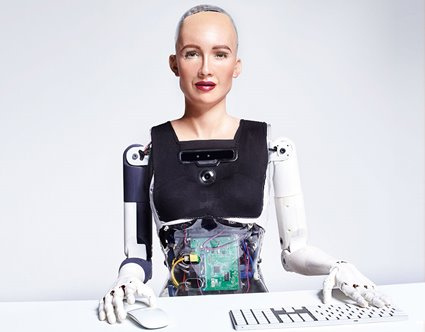
\includegraphics[width=0.28\textwidth]{soa/anthropomorphic}
    }
    \quad
    \subfloat[Zoomorphic robot\label{fig:zoomorphic_robot}]{
        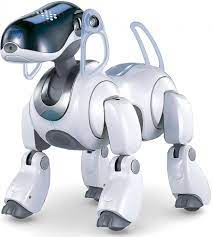
\includegraphics[width=0.28\textwidth]{soa/zoomorphic}
    }
    \quad
    \subfloat[Functional robot\label{fig:functional_robot}]{
        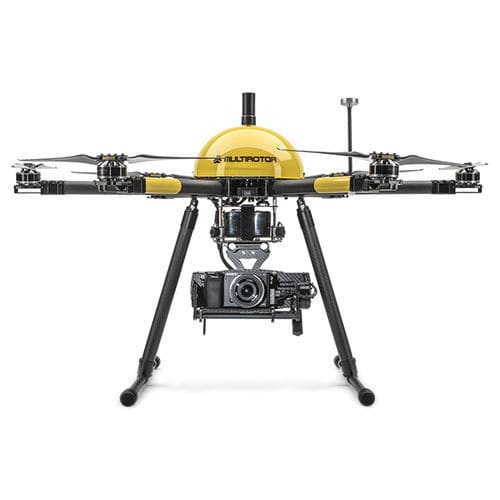
\includegraphics[width=0.28\textwidth]{soa/functional}
    }
    \caption{Robot morphology examples.}\label{fig:robot_morphology}
\end{figure}

In Table~\ref{table:taxonomy_target} we present the type of interaction that we are targeting in this thesis work using the taxonomy described above.

\begin{table}[tb]
\centering
    \begin{tabular}{|p{0.33\textwidth}|m{0.61\textwidth}|}
    \hline
    \rowcolor{bluepoli!40}
    \textbf{Attribute} & \textbf{Values} \\
    \hline \hline
    {\scshape Task Type} & Arbitrary interaction with nano drones in a small indoor environment to investigate Human-Drone relation \\
    \hline
    {\scshape Task Criticality} & Low \\
    \hline
    {\scshape Robot Morphology} & Functional \\
    \hline
    {\scshape Interaction Roles} & Mechanic/Programmer or Operator \\
    \hline
    {\scshape Physical Proximity} &  Any value \\
    \hline
    {\scshape Decision Support} & Available sensors: [proximity (x, y, z), localization (x, y, z), flow (vx, vy), video] \\
    \hline
    {\scshape Time and Space} & Synchronous and Collocated \\
    \hline
    {\scshape Autonomy Level} & Any value \\
    \hline
    {\scshape Amount of Intervention} & Any value \\
    \hline
    \end{tabular}
    \\[10pt]
    \caption[Taxonomy for interaction of target applications]{Categorization of interaction for target applications in our thesis work following the taxonomy proposed by Yanco and Drury~\cite{yanco2004taxonomy}.}\label{table:taxonomy_target}
\end{table}


\section{Human-Drone Interaction}\label{sec:soa_hdi}
Drones, also known as unmanned aerial vehicles (UAVs), are robots capable of flying autonomously or through different control modalities.
Until the early 2000s, drones were complex systems commonly seen in the military world and out of reach for civilians. 
Modern advancements in hardware and software technologies allow the development of smaller, easier-to-control, and lower-cost systems.
Drones are now found performing a broad range of civilian activities, and their usage is expected to keep increasing in the near future.
As drone usage increases, humans will interact with such systems more often; therefore, achieving a natural human-drone interaction is crucial.

Human-Drone Interaction (HDI) can be defined as the study field focused on understanding, designing, and evaluating drone systems 
for use by or with human users~\cite{tezza2019hdi}. Although some knowledge can be derived from the field of HRI, 
drones can fly in 3D space, which essentially changes how humans interact with them, making HDI a field of its own.
This field is relatively new in the research community, but in the last few years, the number of publications about HDI has grown exponentially.

\subsection{The Role of the Human During the Interaction}\label{subsec:hdi_interacction_role}
One of the core topics in the field of HDI is the role of humans during interaction with drones.
Depending on the drone's application and its level of autonomy, humans can play different roles when interacting with drone systems.

When the user pilots the drone to accomplish a given task by directly controlling the drone through a control interface, 
the user is considered an \textit{active controller} of the interaction. In these settings, the user's role is crucial to complete the given task; the drone instead acts as a mere executor of instructions. 
Examples of this type of interaction are waypoint navigation~\cite{hoppe2019droneOS} or artistic exhibitions~\cite{eriksson2020ethicsInMovement}.

The user acts as a \textit{recipient} when they do not control the drone, but they benefit from interacting with it. 
An example of this type of interaction is represented by delivery drones used to deliver a package~\cite{singireddy2018primeAir,hoppe2019droneOS, wingDrones}.

Another type of interaction role is when the drone acts as a \textit{social companion} for the user. 
In this case, the user might or might not be able to control the drone movement, but it holds a social interaction with it.
An example of this type of interaction is represented by Joggobot~\cite{graether2012joggobot}, a drone used as a companion for jogging.

The last type of role the user can play when interacting with a drone is the role of \textit{supervisor}.
Autonomous drones require users to act as supervisors either to pre-program the drone behavior or to 
supervise the flight itself in case of emergency. In this case, examples can be crop monitoring~\cite{dantu2011karma} or aerial photogrammetry~\cite{nex2014uav3Dmapping}, 

\subsection{The Drone's Control Modality}\label{subsec:hdi_drone_control_mod}
Usually, drones expose a control interface that allows users to control their behavior and eventually complete some tasks in the application domain.
Each control interface impacts how the pilot interacts with the drone in various aspects, 
such as training period, accuracy, latency, and interaction distance.

As drones became available to the public, the major drone producers felt the need to change their control modality 
from the standard remote controller to a more natural and easy-to-use interface.
A wide variety of control interfaces are available on the market today, 
ranging from standard remote controllers to very complex and advanced Brain Controlled Drones~\cite{lafleur2013quadcopterBCI}.

Drone's control interfaces can be classified as follows~\cite{tezza2019hdi}:

\textbf{\textit{Remote Controller}} is the standard and most commonly used interface, where the user directly controls the drone movements.
This control modality provides low latency and precise control, but on the other hand, it is less intuitive and usable 
than natural user interfaces. The usability and easiness of this interface strongly depend on the drone's level of autonomy.

\textbf{\textit{Gesture-based interface}} is a control modality where the user pilots the drone with body movements.
Usually, the drone uses a camera or a Kinect device to extract spatial information and recognize postures. 
When users are asked to interact with a drone without any instruction, gesture interaction is the primary choice of most users, 
and this indicates that the training period of this interface is almost close to zero~\cite{cauchard2015droneAndMe}. 
Gesture-based controls have a high latency and lower control precision compared to other control modalities. 
The flight space for drones that use this control method is sensibly reduced since the pilot needs to be close to the drone during the flight.

\textbf{\textit{Speech-based interface}} is a control modality where the user pilots the drone using vocal commands. 
As for gesture-based, this interface is also a natural user interface with a low training period and high usability.
They also share the problems of user proximity and high latency of commands.  

\textbf{\textit{Touch-based interface}} is a control modality where the user is requested to control the drone using his hands. 
The drone usually carries proximity sensors that allow it to receive inputs from the user. 
It is a natural user interface, and, like the others, it has the same pros and cons: high command latency and limited operativity distance.

\textbf{\textit{Brain-computer interfaces}} allows the user to pilot the drone using brain signals~\cite{lafleur2013quadcopterBCI}.
To enable this type of interface, the pilot must wear some form of BCI headset, the most common being 
Electroencephalography (EEG) headsets. These devices measure the brain's electrical activity on a human's scalp, 
which is decoded using machine learning algorithms to control physical systems using brain waves. 
Compared to the others, it is the most complex control interface and has the highest accessibility for users with disabilities. 
The problems in using BCI are the poor control quality and higher training period~\cite{kawala2021summary}. 
Further research in this field will probably lead to more usable and better interfaces.

Interactions can also be combined into \textbf{\textit{multimodal interfaces}}. 
Integrating different interaction methods can combine the advantages of each; however, it can increase complexity and costs.

\subsection{Values and Ethics in HDI}\label{subsec:hdi_ethics}
Drones usually carry cameras, and potentially, they can fly wherever they want; this introduces a lot of issues of privacy~\cite{anderson2012accidentally}.
Given the rapid expansion of such technology, governments worldwide have been caught off guard in recent years. 
Governments tried to quickly create rules and regulations to control the usage of such technology. 
This rapid regulation has, in most cases, limited drones research, slowed their expansion, and reduced their potential.
Research in ethics and values about HDI is responsible for producing accurate and reliable results that should guide 
governments in refining and upgrading drone laws.

Understanding the ethical implications and values of this technology is crucial regarding how humans and drones interact. 
Notably, research studies such as \textit{Ethics in Movement} by S. Eriksson et al.~\cite{eriksson2020ethicsInMovement} and 
\textit{An Exploratory Study of the Use of Drones for Assisting Firefighters During Emergency Situations} by Khan and Neustaedter~\cite{khan2019exploratory} have delved into specific aspects of HDI.

\textit{Ethics in Movement} by S. Eriksson et al.\ explore how ethicality is shaped in interaction between a choreographer, a performer, and a choir of five drones, performing together on the opera stage.
This study highlights that ethics in HDI is not only a matter of general principles but also encompasses how technology concretely influences how we move and experience daily life.

Khan and Neustaedter, in the other paper, conducted a study with citizens who have called 911 and firefighters who respond to a range of everyday emergencies to understand the benefits and challenges of using drones within emergency response.
Their results indicate opportunities for designing drone systems that help people develop trust in emergency response drones and mitigate privacy and safety concerns with more complex drone systems.


\section{Programming Environments}\label{sec:soa_programming_environments}
When developing drone applications, the choice of programming environment is crucial to ensure efficient and reliable software.
The programming environment is intended as all the resources, hardware, and software used to accomplish the tasks of the 
application scenario being developed.

As drone technology expanded, many companies working in the drone field started developing and selling their programming environment. 
Nowadays, most software resources for drone applications are open-source and publicly available. 
We will dive into the scenario of the drone programming environment, understanding the most common and popular solutions 
for developing a drone application. We will then analyze the more complex scenario of swarm applications.

\subsection{Single Drone Programming}\label{subsec:programming_environments_single}
Exploring the programming landscape for a single drone involves navigating through specialized tools and 
frameworks specialized for the development and control of individual drones. 
Whether managing a custom-built drone or utilizing a commercial off-the-shelf (COTS) model, 
creating an effective combination of hardware and software is crucial. 
This section will guide you through essential components and considerations for developing software that governs a 
drone's flight and functionality.

The development of any drone application can be categorized into two main areas: on-board and off-board the drone.

The on-board area comprises all the hardware and the software that composes the drone itself. 
As we can see in Figure~\ref{fig:drone_hw_components}, usually the hardware of the drone includes: 
The frame of the drone, the motors and propellers, the battery and the power distribution unit, the computing unit and the memory unit,
the communication unit and the sensors unit.

\sidecaptionvpos{figure}{c}
\begin{SCfigure}[\sidecaptionrelwidth][tb]
    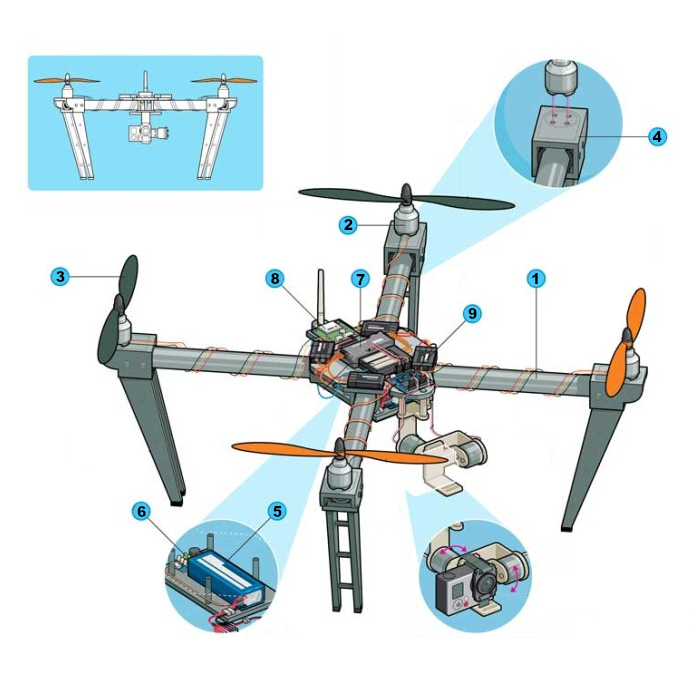
\includegraphics[width=0.5\textwidth]{soa/drone_hw_components}
    \caption[Drone hardware components]{The main hardware components of a drone are: 1. drone's frame, 2. motors, 3. propellers, 4. motor mount, 5. battery, 6. power distribution unit, 7. computing and memory unit, 8. communication unit, 9. sensors unit }
    \label{fig:drone_hw_components}
\end{SCfigure}

The software that runs on the drone, also known as the autopilot software, is usually composed of four main components: the communication unit, the sensing unit, the core control loop unit, and the low-level control unit. 
In Figure~\ref{fig:drone_sw_components}, we can see how the software components cooperate together to achieve a controllable and stable flight.
The communication unit receives and decodes commands from the off-board system; the signal is then transformed into power set-points from the core unit (control loop) with the help of sensor information. 
The sensing unit gathers information from the environment using sensors, translate 
sensor readings into readable values, then send this information to the core unit and to the communication unit to send back telemetry data to off-board systems.

\sidecaptionvpos{figure}{c}
\begin{SCfigure}[\sidecaptionrelwidth][tb]
    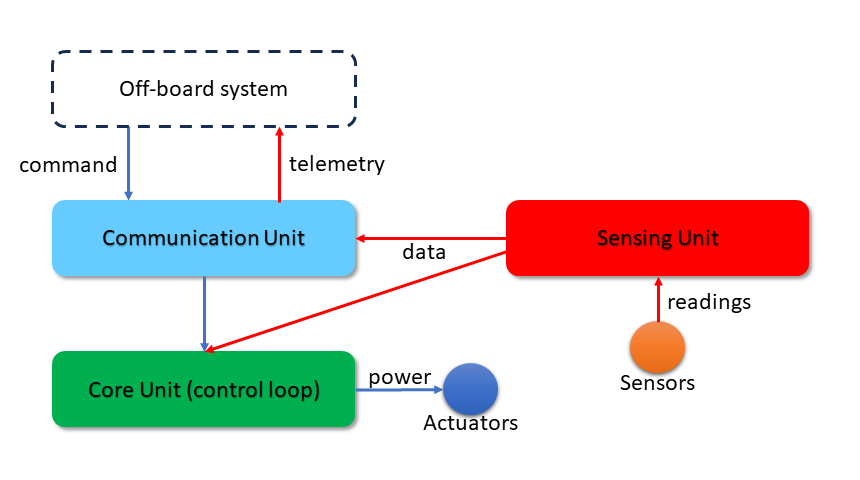
\includegraphics[width=0.7\textwidth]{soa/drone_sw_components.png}
    \caption[Drone software components]{
        The main software components of a drone are: 
        the \textit{sensing unit}, the \textit{communication unit} and the \textit{core unit (control loop)}.
    }\label{fig:drone_sw_components}
\end{SCfigure}

The current landscape of on-board drone solutions ranges from commercial off-the-shelf (COTS) to entirely custom solutions.
Commercial producers of drones like Parrot~\cite{parrot}, DJI~\cite{dij}, and 3DR~\cite{3DR} usually sell COTS solutions where all the hardware resources are supplied
with the software needed to run the drone.
Depending on the application, these bundled solutions may not be enough; if this is the case, 
the developer then needs to manually select each hardware component, control the compatibility with each other, 
and then select (or develop) the software that allows the drone to fly.

Some producer sell also intermediate solutions~\cite{pixhawk, px4, cube, navio2} between COTS and the completely custom one.
These solutions are composed of a microcontroller with usually the basic sensors that compose the 
Inertial Measurement Unit (IMU) and the autopilot software. 
These solutions are then extensible with other custom hardware; they provide programming tools to program the 
behavior of the drone during the flight.

%  TODO: reference chapter tools (section bitcraze) 
Regarding our setup, the on-board system that we used is a nano drone named Crazyflie 2.1, produced by Bitcraze; 
it is a COTS solution but with a lot of space for customization for both hardware and software components.

Off-board the drone, the environment is strongly related to the application scenario, and, in particular, it depends on the level of 
autonomy request for the drone, the flight area dimension, and the complexity of the operation.

Despite the heterogeneity of off-board systems, we can consistently identify two main components in most scenarios: a control unit and a communication unit. 
In most common situations, control and communication units are hosted on a single device.
Example of these devices are remote controls (Figure~\ref{fig:ground_station_controller}), smartphones (Figure~\ref{fig:ground_station_controller})
or a computer that acts as base (ground) station (Figure~\ref{fig:ground_base_station}).
When the scenario is more complex and the fight area is very broad, 
we can have a distributed ground network of control and communication units (Figure~\ref{fig:ground_station_distributed}).
Additionally, in combination with a distributed ground network, a sensor network can also be deployed to gather more information about the drone in its environment (Figure~\ref{fig:ground_station_distributed_with_sensor}). 
For example, the sensor network can be composed of sensors that collect atmospheric data, allowing for a better knowledge of the environment in which the drone is deployed. 

\begin{figure}[tb]
    \centering
    \subfloat[Remote control\label{fig:ground_station_controller}]{
        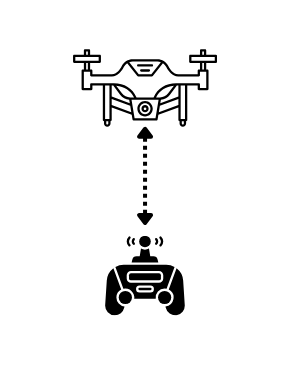
\includegraphics[width=0.25\textwidth]{soa/ground_station_controller}
    }
    \quad
    \subfloat[Smartphone\label{fig:ground_station_smartphone}]{
        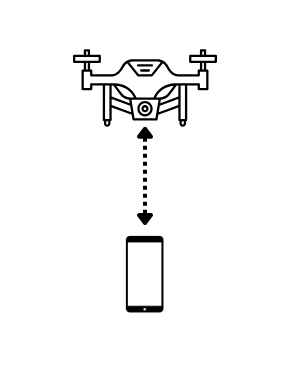
\includegraphics[width=0.25\textwidth]{soa/ground_station_smartphone}
    }
    \quad
    \subfloat[Base Station\label{fig:ground_base_station}]{
        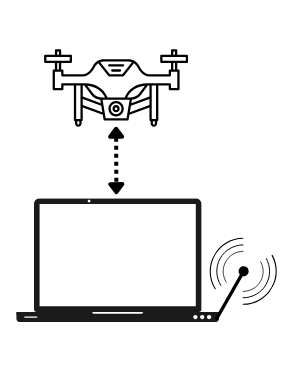
\includegraphics[width=0.25\textwidth]{soa/ground_base_station}
    }
    \quad
    \subfloat[Distributed ground network\label{fig:ground_station_distributed}]{
        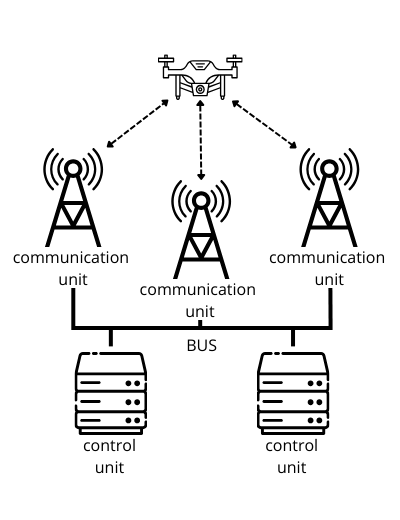
\includegraphics[width=0.35\textwidth]{soa/ground_station_distributed}
    }
    \quad
    \subfloat[Distributed ground network and sensor network\label{fig:ground_station_distributed_with_sensor}]{
        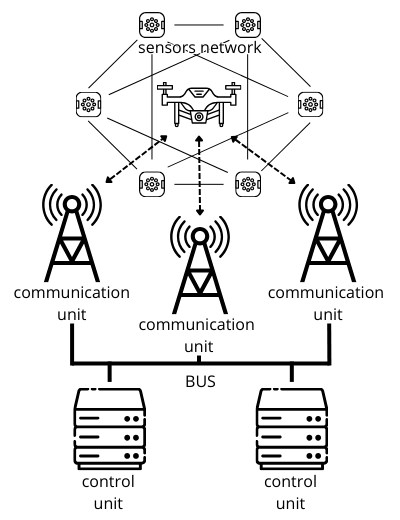
\includegraphics[width=0.35\textwidth]{soa/ground_station_distributed_with_sensor}
    }
    \caption[Off-board ecosystem]{Off-board ecosystem}\label{fig:off_board_ecosystem}
\end{figure}

Communication technology and infrastructure are critical topics that can introduce potential issues 
in the off-board environment when it is inadequate for the application scenario.
In particular, depending on the flight area's dimension, location, and topography, appropriate technology and communication infrastructure must be deployed to have a properly working drone.

As highlighted in Figure~\ref{fig:off_board_ecosystem}, the communication infrastructure can be single or distributed.
The former is more straightforward to implement and deploy but can be not enough when the flight area is too broad or the topography is irregular; 
the latter is much more complex but allows for covering all the possible application scenarios.

The most commonly used communication technology in the drone's field are Wi-Fi, radio, Bluetooth, and cellular network~\cite{pantelimon2019surveyCommunication}. 
Table~\ref{table:communication_technologies} summarizes the most common communication technologies and their characteristics.
Even if the research frontier for drone communication is mainly focused on cellular, in particular the 5G network~\cite{sharma2020communication},
none of the technologies prevails, but the choice depends on the application scenario. 
Cellular

can be a great solution around highly populated areas, while another technology must be considered in rural locations.


\begin{table}[tb]
    \centering
        \begin{tabular}{|c|c|c|c|c|}
        \hline
        \rowcolor{bluepoli!40}
        \textbf{Technology} & \textbf{Range} & \textbf{Weight} & \textbf{Complexity} & \textbf{Cost} \\
        \hline \hline
        Wi-Fi & MED [100m] & MED & HIGH & MED \\
        \hline
        Radio & SHORT-LONG [10-1000m] & LOW & LOW & LOW \\
        \hline
        Bluetooth & SHORT-MED [<25m] & LOW & MED & LOW \\
        \hline
        Cellular & LONG [8000m] & LOW & HIGH & MED \\
        \hline
        \end{tabular}
        \\[10pt]
        \caption[Communication technologies]{Communication technologies used in drone applications~\cite{pantelimon2019surveyCommunication}}\label{table:communication_technologies}
    \end{table}

The software that runs off-board is usually apt to coordinate all the resources of the environment to finally achieve and 
complete the task needed for the application. When using COTS or intermediate solutions, the vendors usually provide the 
hardware and software that compose the off-board ecosystem.

Figure~\ref{fig:easyfly_offboard_ecosystem} shows the off-board environment used in this work. 
It consists of a single base station with a USB dongle radio operating in a 2.4GHz band using a custom communication protocol named CRTP (see Section~\ref{subsec:crazyradio}). 
In substitution of a sensor network, we have an external positioning system (Lighthouse positioning system) composed of two base stations that beam the flight space with infrared, enabling the drone to measure its position by knowing the direction of infrared rays (see Section~\ref{subsec:lighthouse_hardware}).

\begin{wrapfigure}{H}{0.3\textwidth}
    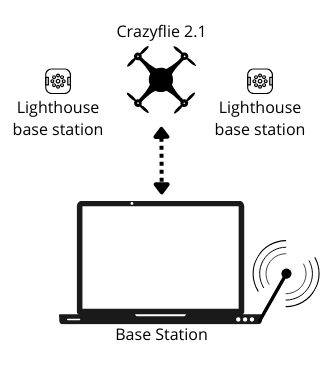
\includegraphics[width=0.3\textwidth]{soa/easyfly_offboard_ecosystem}
    \caption{EasyFly off-board ecosystem.}\label{fig:easyfly_offboard_ecosystem}
\end{wrapfigure}

A widespread problem encountered while dealing with drones is the testing phase of the application in a real environment. 
As in any other programming environment, drone programming is not immune to code bugs or hardware problems. 
Unfortunately, when an error arises, the drone will usually crash; in some unfortunate cases, some parts will break and need to be replaced. 
Therefore, testing drone applications is a very expensive task both in terms of economic resources and in terms of time. 

To overcome this limitation, the main drone producers have developed and distributed a simulation environment that allows 
testing the software before going into a real scenario. 
A simulation environment allows running the code written for the planned mission in a graphical simulation that shows the drone performing the tasks. 
Modern simulation environment~\cite{sphinx, DIJflightSimulator} usually takes into consideration atmospheric phenomena like pressure and wind to make the simulation 
closer to the real deployment environment.

In our work, we built our custom simulation tool, allowing us for a better evaluation of the work itself and, moreover, allowing  
users of our programming environment to have all the benefits of using a simulation environment (see Section~\ref{subsec:simulation_environment}).

\subsection{Swarm Programming}\label{subsec:swarm_programming}
In modern drone applications, where the tasks to achieve are complex, and the application has to be reliable, a common approach is 
to deploy multiple drones to complete the requested task collectively. This approach is completely different from single 
drone programming; in fact, swarm programming introduces new challenges and a different approach to achieving the tasks of the application.

Swarm programming is a branch of the more general swarm engineering which tries to take advantage of using multiple resources to 
achieve the application goal with better performance.

Swarm robotics and, more in general, swarm engineering is an emerging discipline that aims at defining systematic 
and well-founded procedures for modeling, designing, realizing, verifying, validating, operating, and maintaining 
a swarm robotics system. Taking inspiration from the self-organized behaviors of social animals, it makes use of simple 
rules and local interactions to design robust, scalable, and flexible collective behaviors for the coordination of large numbers of robots.
The inspiration that swarm robotics takes from the observation of social animals (ants, bees, birds, fish, …) is that starting from simple individuals,
they can become successful when they gather in groups, exhibiting a sort of swarm intelligence~\cite{bonabeau1999swarm}.

In particular, the behavior of social animal groups appears robust, scalable, and flexible. 
Robustness is the ability to cope with the loss of individuals. 
In social animals, robustness is promoted by redundancy and the absence of a leader. 
Scalability is the ability to perform well with different group sizes. 
The introduction or removal of individuals does not result in a drastic change in the performance of a swarm. 
In social animals, scalability is promoted by local sensing and communication. 
Flexibility is the ability to cope with a broad spectrum of different environments and tasks. 
In social animals, flexibility is promoted by redundancy, simplicity of the behaviors, and mechanisms such as task allocation.

Two great examples in the current literature of swarm engineering are Proto~\cite{bachrach2010proto} and Meld~\cite{ashley2007meld}. 
The former is a spatial computing language that allows programming swarms of robots starting from a mathematical model called amorphous medium.
The latter is a declarative programming language that uses logic programming to enable swarm programming.
Both languages directly take the swarm programming from the point of view of aggregate behaviors, i.e., their approach is to program the entire
swarm behavior instead of programming every single component separately.

When swarm robotics is applied in the field of drones, given the high dynamism in the movements of this type of robot, 
the swarm management and control is much more complex with respect to the single drone, 
but the capability of the swarm may increase the application's performance.

In the first place, the swarm, compared to the single drone, can provide a higher availability.
A single drone has a limited flight time, so its batteries need to be recharged or replaced. A swarm instead can dynamically 
deploy and retire drones to be always active on the field. In addition, a swarm can also scale when the request 
increases, e.g., a phenomenon to sense has a peak of occurrence~\cite{dantu2011karma}. 
In the same situation, a single drone application can miss the peak of the phenomena because, for example, it can be stuck at the charging station.

With swarms, the goal of the application is usually defined as a swarm goal.
Swarm goals are high-level goals whose achievement is independent of the success or the failure of the single task of a swarm component.
The separation between application (swarm) goals and drone tasks allows the application to be scalable and fault-tolerant.
Of course, the advantages of the swarm with respect to the single drone hide inside a huge complexity.
As the number of components of the swarm increases, the complexity of managing all of them increases, 
introducing a consistent overhead that can affect the application's performance.
As in any other engineering problem, we must select and identify the most suitable swarm size for the application to realize.

Depending on the application domain, we can adopt different strategies for coordinating the resources available.
We can identify three main programming models that can be applied to swarm programming in the field of drones: drone-level programming, swarm programming, and team-level programming.

Drone-level programming is the most straightforward approach; it expects to develop a single application for each component of the swarm, 
taking into account all the possible interactions between them. 
This finest grain method allows an entirely independent, customizable, and deterministic single-drone behavior. 
Since the application has a swarm goal that is not directly related to the single drone's task, 
with this method, it is usually tricky to use all the swarm resources efficiently to reach the general goal. 
Moreover, it has been proven~\cite{mottola2014team, dantu2011karma} that this method is indeed the most complex of the three in terms of programming effort.

Swarm programming~\cite{quigley2009ros}, on the other hand, allows writing a single set of rules that are common for all drones, and then every single drone 
executes that instruction in its local state. The swarm programming model explicitly forbids a shared or global state.
This programming model is easier to use and to set up and scale up with multiple drones, but it is challenging to represent tasks that require explicit drone coordination.

Team level programming~\cite{mottola2014team} is a programming model in between swarm and drone level programming, 
in which users express sophisticated collaborative sensing tasks without resorting to individual addressing 
and without exposure to the complexity of concurrent programming, parallel execution, scaling, and failure recovery.
The model can be viewed as a set of tasks that must be performed by a set of drones subject to particular timing and spatial constraints~\cite{mottola2014team}.

Our work does not address the complexity of swarm programming, although our programming environment, EasyFly, allows for the deployment of multiple drones (see Chapter~\ref{ch:conclusions}).

\chapter{Tools}
\label{ch:tools}
The main resource used in this work is Crazyflie, an open platform produced by Bitcraze~\cite{bitcraze} 
that offers an ecosystem of products and open-source libraries that allow people to develop new functionality for aerial drones. 

The key feature of this platform is that it offers a set of expansion decks that can extend the capabilities of the drone with new sensors. 
Expansion decks can be mounted on the drones very easily, and they are immediately ready to be used to compose the desired configuration in the application of interest.
Given its modularity and high versatility, this platform perfectly fits as a baseline for developing an easy, high-level environment for programming drones. 

The aim of this chapter is to present an overview of the Crazyflie platform to provide basic knowledge of its tools and surrounding environment.

% We will first present all the hardware used in this work, then we will give an overview of all the software libraries that compose the platform and finally we will describe in detail the main software components.

\section{Ecosystem Overview}\label{sec:ecosystem_oveerview}
The Crazyflie platform comprises a set of devices and tools to allow building drone applications. 
It has a modular architecture that makes it possible to build very versatile systems that are adaptable to many situations. 
In Figure~\ref{fig:bitcraze_ecosystem}, we can see an overview of the ecosystem of the entire platform.

The ecosystem of this platform gravitates around its leading actor: the Crazyflie 2.1 nano drone. 
In the basic settings, the drone has minimal sensors and actuators that allow it to fly. 
To empower the drone capabilities, the platform makes available a set of expansion decks that give the drone additional sensors, making it possible to adapt it to many possible situations.


\sidecaptionvpos{figure}{c}
\begin{SCfigure}[\sidecaptionrelwidth][h]
    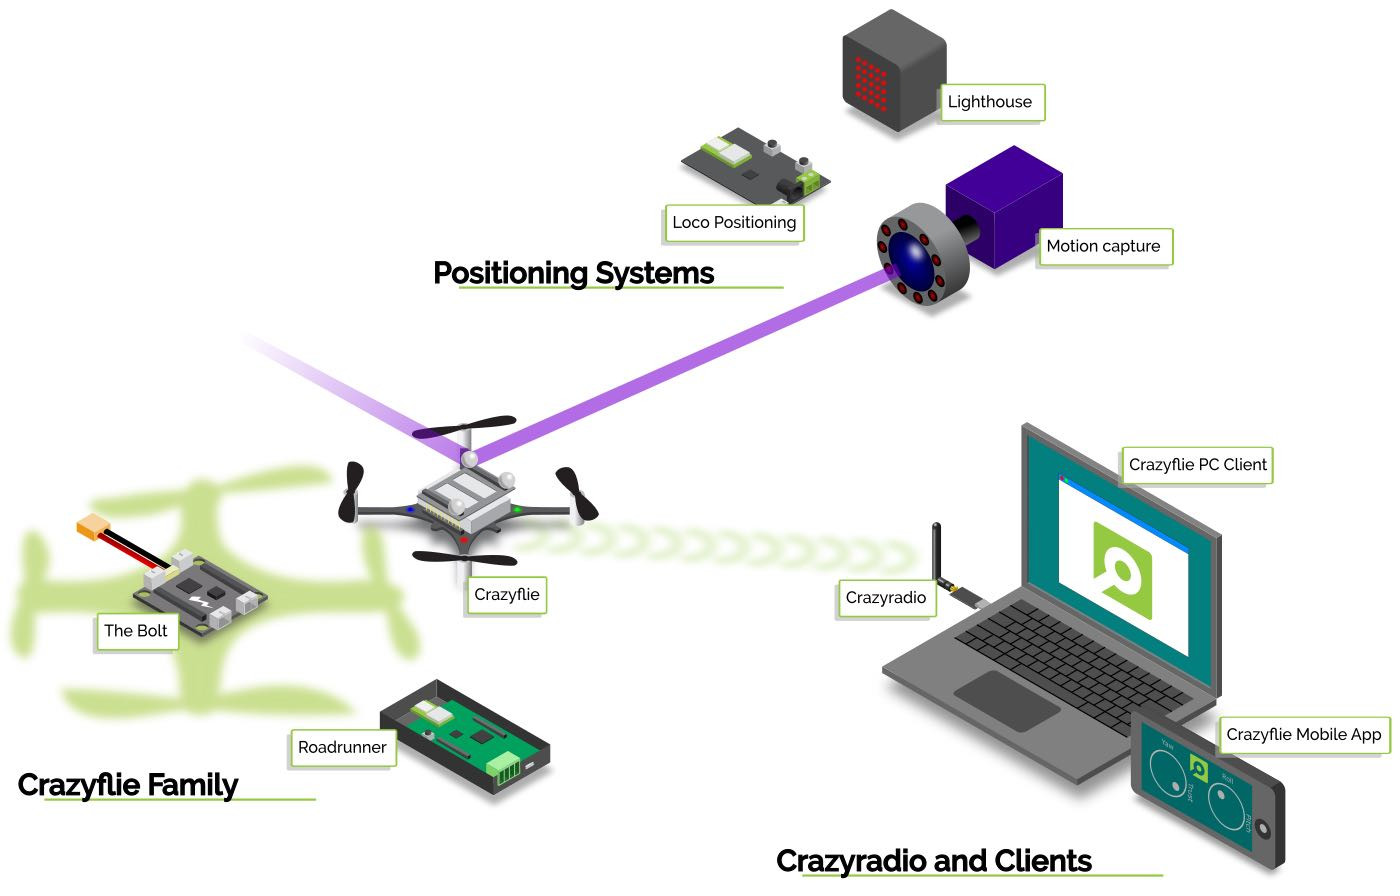
\includegraphics[width=0.5\textwidth]{tools/system_overview}
    \caption[Bitcraze Ecosystem overview]{This picture represents an overview of the Bitcraze Ecosystem~\cite{bitcraze}}
    \label{fig:bitcraze_ecosystem}
\end{SCfigure}


To coordinate the drone's operations, the platform needs a ground station that can be hosted on any computer 
with a Python script interpreter or a mobile phone with a dedicated App installed. 

The communication between the quadcopter and the ground station is handled using a dongle USB (CrazyRadio) or through Bluetooth when using the mobile App.

The platform also offers multiple absolute positioning systems that allow the drone to have better position estimation in an absolute coordinate system.

\section{Hardware}\label{sec:crazyflie_hardware}
In this section, we will provide an overview of the hardware components of the entire Crazyflie platform. 
We will first analyze the characteristics of the Crazyflie quadcopter used in this work, and then we will briefly introduce the relevant expansion decks. 
We will then give an overview of the hardware components that compose the absolute positioning system adopted for the work: the Lighthouse positioning system.

\subsection{The Quadcopter}\label{subsec:the_quadcopter}
Bitcraze produces a family of drones with similar hardware and firmware but different sizes and properties. 
The target for this work is the principal component of this family, the Crazyflie 2.1, a tiny and versatile quadcopter with a solid and modularized design that falls into the category of nano-drones.

As described in Section~\ref{sec:the_solution}, nano-drones are the most suitable typology for conducting investigations around HDI. 
The modular approach owned by Crazyflie 2.1 constitutes another key advantage in the field of human-drone interactions; 
the user can easily change the setup to address any possible situation. 

This drone has many hardware components hosted on a single, compact, light base. 
We can identify four main units: Computing Unit, Motor Unit, Sensor Unit, and Power Unit.

The core of the drone is composed of two Micro Controller Units (MCUs): 
The first is an STM32F4 MCU that handles the main Crazyflie firmware with all the low-level and high-level controls. 
The second MCU, NRF51822, handles all the radio communication and power management. 

The motor unit of the Crazyflie 2.1 consists of four Coreless DC motors with plastic propellers fixed at the corners of the base with the help of plastic supports.
To control the flight, the drone is equipped with two sensors: a BMI088 sensor, which measures the acceleration along the three coordinates of space plus the angular speed, 
and a BMP388 sensor, which is a high-precision pressure sensor.
The sensor unit of the Crazyflie 2.1, also known as the Inertial Measurement Unit (IMU), is minimal and provides the minimum data that allows the drone to have an almost stable flight.

Its design is robust and simple, easing the assembly and maintenance of its components.
Finally, the power unit is constituted by a 240mAh LiPo battery that allows a flight duration of about 7 minutes. 
The total weight of the drone is 27 grams, and it can lift a payload of 15 grams~\cite{crazyflie}. 


\subsection{Expansion Decks}\label{subsec:expansion_decks}
With only two sensors composing the IMU, the drone has a limited capacity to understand the surrounding environment. 
To overcome this limitation, the drone can be equipped with additional decks that extend its capabilities in sensing, positioning, and visualization.
The platform offers a variety of expansion decks, but for the purpose of our work, only a subset of them has been selected.
Figure~\ref{fig:decks} shows the expansion decks selected, particularly those that can enable in some way the human-drones interaction.

\begin{figure}[h]
    \centering
    \subfloat[Flow deck v2\label{fig:flow_deck}]{
        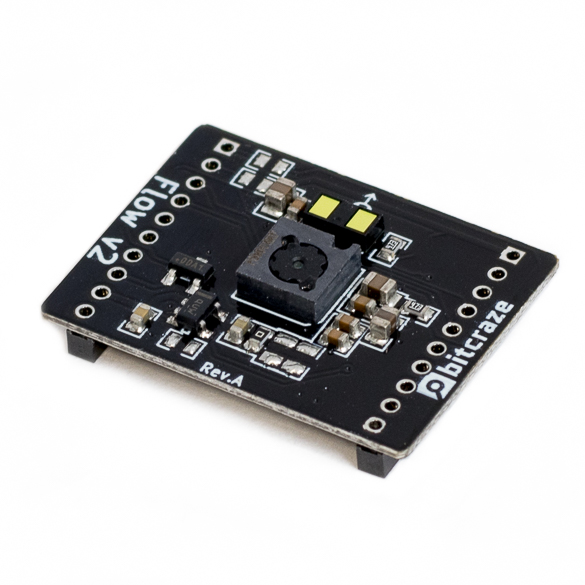
\includegraphics[width=0.16\textwidth]{tools/flow_deck_v2}
    }
    \quad
    \subfloat[Z-ranger deck v2\label{fig:z_ranger_deck}]{
        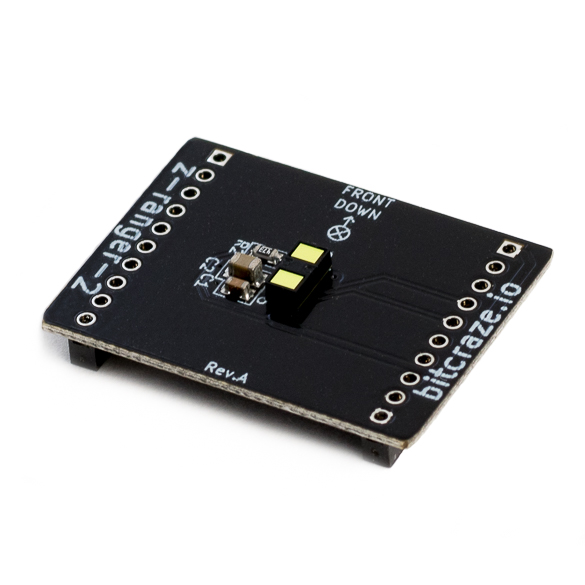
\includegraphics[width=0.16\textwidth]{tools/z-ranger_v2}
    }
    \quad
    \subfloat[Multi-ranger deck\label{fig:multi_ranger_deck}]{
        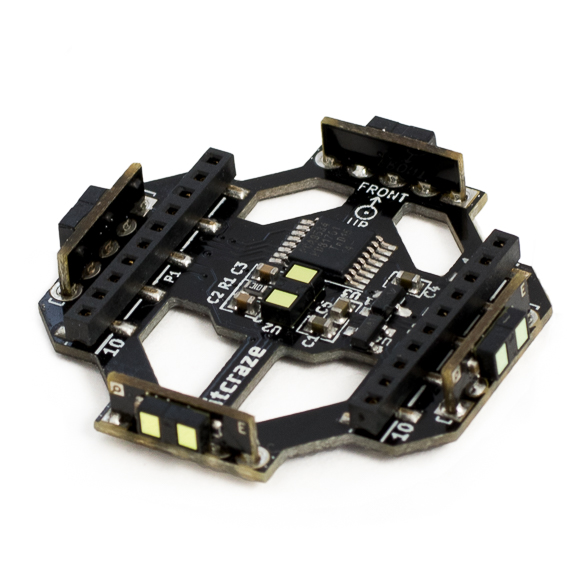
\includegraphics[width=0.16\textwidth]{tools/multi-ranger_deck}
    }
    \quad
    \subfloat[Lighthouse positioning deck\label{fig:lighthouse_deck}]{
        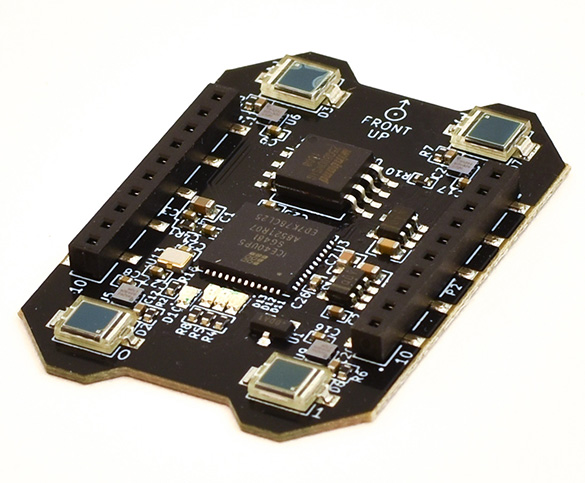
\includegraphics[width=0.16\textwidth]{tools/lighthouse_deck}
    }
    \quad
    \subfloat[AI-deck 1.1\label{fig:ai_deck}]{
        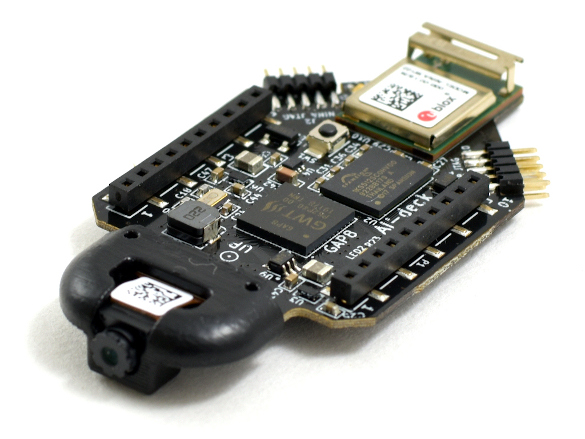
\includegraphics[width=0.16\textwidth]{tools/ai-deck}
    }
    \caption{Expansion decks of Crazyflie 2.1}\label{fig:decks}
\end{figure}


{\bfseries \scshape Flow deck v2}\label{deck:flow}:\\*
The Flow deck (Figure~\ref{fig:flow_deck}) allows the Crazyflie to understand when it moves in any direction. 
It mounts two sensors: the VL53L1x ToF measures the distance to the ground with high precision up to 4 meters, and the PMW3901 optical flow sensor measures the relative velocity in the x-y plane relative to the ground. 
This expansion deck is a relative positioning system that lets the drone know its position relative to its take-off point.

{\bfseries \scshape Z-ranger deck v2}\label{deck:z_ranger}:\\*
The Z-ranger deck (Figure~\ref{fig:z_ranger_deck}) is a simplified and cheaper version of the Flow deck v2.
It only measures the distance from the floor up to 4 meters using the usual laser sensor VL53L1x ToF.

{\bfseries \scshape Multi-ranger deck}\label{deck:multi_ranger}:\\*
The Multi-ranger deck (Figure~\ref{fig:multi_ranger_deck}) gives the Crazyflie the capability to sense the space around it and react when something is close and for instance, avoid obstacles.
This is done by measuring the distance to objects in the following five directions: front, back, left, right, and up with mm precision up to 4 meters, using five VL53L1x ToF sensors.


{\bfseries \scshape Lighthouse positioning deck}\label{deck:lighthouse}:\\*
The Lighthouse deck (Figure~\ref{fig:lighthouse_deck}) is part of the Lighthouse absolute positioning system (See Section~\ref{subsec:lighthouse_hardware}). 
It comprises four TS4231 IR receivers and an ICE40UP5K FPGA to process the signal received.
This expansion deck lets the drone know its position in an absolute coordinate system.

{\bfseries \scshape AI-deck 1.1}\label{deck:ai}:\\*
The AI-deck 1.1 (Figure~\ref{fig:ai_deck}) extends the computational capabilities and will enable complex artificial intelligence-based workloads to run onboard, with the possibility to achieve fully autonomous navigation capabilities. 
It mounts an Himax HM01B0 (ultra-low power \(320 \times 320\) monochrome camera), GAP8 (ultra-low power 8+1 core RISC-V MCU), NINA-W102 (ESP32 module for WiFi communication), and it has 512 Mbit HyperFlash and 64 Mbit HyperRAM memories. 


\subsection{Crazyradio PA}\label{subsec:crazyradio}
As previously described, the Crazyflie platform expects two nodes of computation: the ground station and the Crazyflie 2.1 itself. 
To communicate with the Crazyflie 2.1, which has an integrated radio, the ground station needs an external radio dongle. 
The platform provides a low-latency and long-range USB radio dongle, the Crazyradio PA.

The CrazyRadio PA is based on the nRF24LU1+ from Nordic Semiconductor, and it features a 20dBm power amplifier giving a range of up to 1km (line of sight).
The dongle comes pre-programmed with Crazyflie's compatible firmware.

The communication protocol used to communicate is the Crazy Radio Transfer Protocol (CRTP), 
which is a custom communication protocol of the Crazyflie platform. %(See section 3.7). TODO: understand if there is this section

\subsection{Lighthouse Positioning System Hardware}\label{subsec:lighthouse_hardware}
The Lighthouse positioning system is one of the possible solutions that Bitcraze offers to have an absolute positioning system for understanding the drone's coordinates inside the flight space. 
The hardware of this system is composed of 2 or more HTC-Vive/SteamVR Base Station 2.0. 
The role of these base stations is to lighten up the flight space with periodic infrared (IR) beams.

Onboard the Crazyflie 2.1, the Lighthouse expansion deck allows it to capture these IR beams thanks to four TS4231 IR receivers. 
The signal captured is then passed to an ICE40UP5K FPGA that computes the angle of incidence of the IR rays with signal processing. 
The position and the pose of the Craziflie are then finally computed from the main MCU of the Crazyflie 2.1 % (See section 3.4.x).TODO: understand if there is this section


\section{Software Libraries}\label{sec:software_libraries}
As previously anticipated, the Crazyflie environment is completed by a set of open-source libraries, 
publicly available on GitHub, which allow people to program all its components and devices, 
develop new features, or upgrade existing ones. Each library targets a specific system component and is completely independent of all the others. 
This section will briefly describe the two main libraries used as a baseline for our work. 

\subsection{crazyflie-lib-python}\label{subsec:crazyflie_lib_python}
The crazyflie-lib-python (cflib in short)~\cite{crazyflie-lib-python} is a software repository that consists of a Python library for programming scripts that control the behavior of the Crazyflie 2.1.
The library provides the base facilities to allow users to define the desired drone behavior in a Python script, abstracting from the low-level control mechanism.

As shown in Figure~\ref{fig:software_libraries}, the Python scripts are executed on the ground station.
The library contains the code to create communication packets sent through the Crazyradio reaching the Crazyflie, which will eventually execute the commands requested. 

\subsection{crazyflie-firmware}\label{subsec:crazyflie-firmware}
The crazyflie-firmware~\cite{crazyflie-firmware} is a software repository that contains all the firmware of Crazyflie 2.1. 
The firmware is written in C++ and handles the main autopilot on the STM32F4; it contains the driver of each possible expansion deck and controls all the communication on the opposite side of the cflib.


\begin{figure}[h]
    \centering
    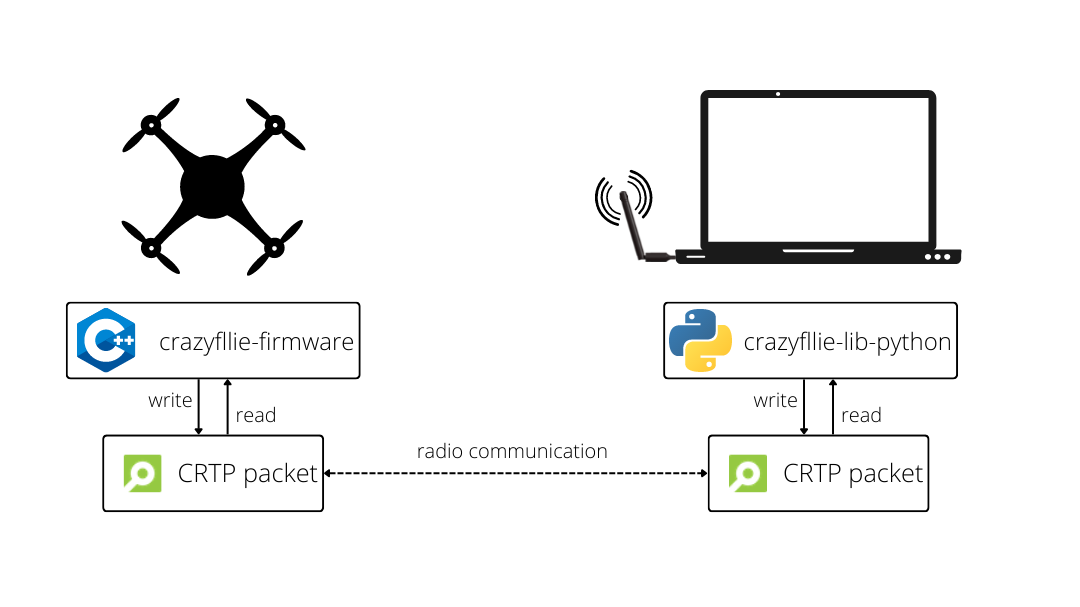
\includegraphics[width=0.9\textwidth]{tools/software_libraries}
    \caption[Software libraries integration]{
        The two main software libraries are \textit{crazyflie-firmware} and \textit{crazyflie-lib-python}. 
        The former, written in C++, runs on the drone; the latter, written in Python, runs on the base station. 
        The communication protocol that enables the cooperation of the two is the Crazy Radio Transfer Protocol (CRTP)}\label{fig:software_libraries}
\end{figure}


\section{Positioning Systems}\label{sec:positioning_systems}
Positioning systems represent the core sensing task of every drone application. 
Knowing the drone's position in the flight space is essential for achieving any possible goal.
We can identify two main categories of positioning systems: relative and absolute. 

Relative positioning systems are the simplest: starting from the drone's position at take-off, they estimate the position during the flight on the base of the movements made by the drone in the flight space. 
The measurement of the movements is usually made with the IMU (Inertial Measurement Unit) or with some additional sensors that track the difference in position over time.

The main issue related to this type of positioning system is that the error continually accumulates, and after a certain period of flight, they
can lead to consistent mispositioning.

Absolute positioning systems provide coordinates that define the exact location of an object within a specific coordinate system. 
These systems typically rely on external references or signals from fixed environmental points.
The sampling of the position in this type of positioning system is independent of any initial measurements, so the error in the positioning usually does not accumulate over time.


The Crazyflie platform offers multiple positioning systems, both absolute and relative. 
To select the best system for building our programming environment, we analyzed the following metrics for each possibility that the platform offered:
\begin{itemize}
    \item Relative or Absolute Positioning System
    \item Accuracy in sampling
    \item Cumulative of the error during time
\end{itemize}


\subsection{Relative Positioning Systems}\label{subsec:relative_positioning_systems}
The Crazyflie platform offers three relative positioning systems. 
The first system is represented by the Inertial Measurement Unit, which is provided on the base drone without expansion decks. 
From our experience, this system has very poor accuracy and cannot be used as the only positioning system of the entire application.
However, it contributes its information to obtain the position estimate.

The Z-ranger deck (See~\ref{deck:z_ranger}) is another positioning system that the platform offers; it provides an estimate only for the z-coordinate with pretty good accuracy, but, as typical for every relative positioning system, it has a high cumulative error during the time. 

The Flow deck v2 (See~\ref{deck:flow}) represents an empowered version of the Z-ranger, a positioning system capable of measuring the distance from the takeoff point for the three coordinates x, y, and z. 
This last system has a good sampling accuracy and an acceptable cumulative error rate over time. 
Flow deck v2 is the only relative positioning system that allows the Crazyflie to fly with acceptable precision in the flight space.


\subsection{Absolute Positioning Systems}\label{subsec:absolute_positioning_systems}
The environment provides three different absolute positioning systems solutions with different characteristics, performance, and costs. 

The first solution proposed, the Loco Positioning System (LPS), is based on Ultra Wide Band radio that is used to find the absolute 3D position of objects in space. 
Similarly to a miniature GPS system, it uses a set of Anchors, namely Loco positioning nodes (from 4 up to 8), that act as a GPS satellite, and a Tag, 
namely, the Loco positioning deck, which acts as a GPS receiver. 
As indicated in the specification of this system, the accuracy of this system is probably the main limitation and is estimated to be in the range of 10 cm. 

The second solution proposed is the Motion Capture System (MCS), which uses cameras to detect markers attached to the Crazyflies. 
Since the system knows the layout of the markers on the drone, it is possible to calculate the position and orientation of the tracked object in a global reference frame. 
It is a very accurate positioning system, but the two main limitations are that the native environment provides only the markers and relies on third-party systems for the entire MCS. 
Moreover, the position is computed in an external node and needs to be sent to the Crazyflie, increasing the communication load.

The last solution is the Lighthouse positioning system (Lighthouse), the newest introduced in the environment and selected for the work because it overcomes all the limitations of the previous.
Lighthouse is an optically-based positioning system that allows an object to locate itself with high precision indoors. 

The system uses the SteamVR Base Station (BS) as an optical beacon. 
They are composed of spinning drums that shine the flight space with infrared beams in a range of 6 meters. 

The Crazyflie, on the other hand, with a Lighthouse positioning deck with four optical IR receivers (photodiode), can measure the angle of incidence of the IR beams. 
Knowing the position and orientation of the BS enables the Crazyflie to compute its position onboard in global coordinates. 
The knowledge of the position and the orientation of the BS is called system geometry and is composed of a vector in the three dimensions and a rotation matrix. 



\section{State Estimate and Control}\label{sec:state_estimate_and_control}
All the information given by the positioning systems and by the additional decks are simply data,
to become useful, they need to be used cleverly to control the drone's stability and make it possible to fly. 

This section will describe the principal software components that act in the control loop, enabling the drone to fly.
In the Crazyflie platform, the control loop is managed inside the Crazyflie firmware (See~\ref{subsec:crazyflie-firmware}) from the sensor read to the motor thrust.
In Figure~\ref{fig:control_loop}, we can see a representation of the control loop of the Craziflie 2.1. 

\begin{figure}[h]
    \centering
    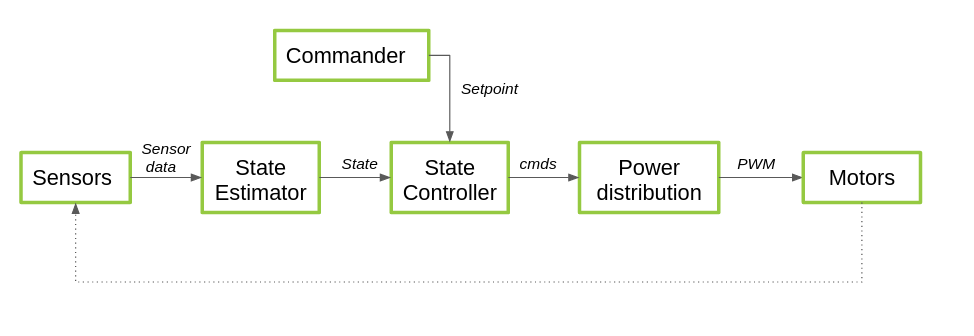
\includegraphics[width=0.9\textwidth]{tools/control_loop}
    \caption[Craziflie's control loop]{
        The control loop of the Craziflie 2.1~\cite{bitcraze}
    }\label{fig:control_loop}
\end{figure}

As in any feedback control system, also for the Crazyflie control loop, we can identify two principal components in Crazyflie 2.1: the state estimator and the state control. 
The synergy between the state estimate and the state control in a control loop is fundamental for achieving accurate and effective system control. 

The state estimator is responsible for computing the best possible estimate of the system's current status.
This component inside the Crazyflie 2.1 firmware has two concrete implementations with different performances and accuracy:
\begin{itemize}
    \item Complementary Filter
    \item Extended Kalman Filter (EKF)
\end{itemize}

The Complementary Filter is a very lightweight and efficient state estimator. 
It can only partially use the available sensors; in particular, it uses only data from the IMU and the ToF sensor (Flow deck or Z-ranger).
The estimated output is only a portion of the Crazyflie state: the Attitude (roll, pitch, and yaw) and the z coordinate relative to the starting point.

The EKF is a recursive filter that estimates the current state of the Crazyflie based on incoming measurements (in combination with a predicted standard deviation of the noise), the measurement model, and the model of the system itself. 
It is a step up in complexity with respect to the other estimator; it accepts all the possible sensors' data as input. 
If enough sensor data are available, it can compute a complete state estimation as output: Attitude, Position, and Velocity in all directions.
The choice of which state estimator to use can be forced by the user or automatically set. 
By default, the firmware uses the lighter Complementary Filter and switches to the EKF if more sensors are available.

The state control uses this estimate to elaborate the actions needed to change the current state to a target state.
On the Craziflie's 2.1 firmware, we have three possible alternatives, ordered by complexity:
\begin{itemize}
    \item Proportional Integral Derivative Controller (PID)
    \item Incremental Nonlinear Dynamic Inversion Controller (INDI)
    \item Mellinger controller
\end{itemize}


\section{Flight Control}\label{sec:flight_control}
On the other side of the communication channel, the ground station needs a way to interact with the drone and give information on which actions to take to fly in the desired way.

Inside the cflib the one responsible for controlling the flight is a module named Commander Framework.
The Commander Framework can be viewed as composed of two layers:

The first layer provides low-level operations that allow writing setpoints and sending them with the custom CRTP protocol.

The second layer, built upon the first, is more abstract and adds some general functionalities, e.g., take-off, land, and move-to.

\chapter{Extended Crazyflie}
\label{ch:ecf}
From this chapter, we will start presenting our contribution to the current state of the art.
In particular, we will start our journey by outlining the big picture; then, we will enter into the detail of the various parts of EasyFly, understanding the design principles and motivations behind each part.

As described in the previous chapter (see Chapter~\ref{ch:tools}), we built our EasyFly programming environment upon the Crazyflie platform produced by Bitcraze~\cite{bitcraze}.
For this reason, we will use and extend the tools offered by the platform.

Specifically, we extend the capabilities of the Crazyflie platform through the development and integration of our programming environment.
Here is where the Extended Crazyflie (ECF) comes into play: the simplest but most effective component of EasyFly. 
This component is a centralized unit that wraps and links together all the functionality of our programming environment. 
It acts as a bridge between the Crazyflie platform and the core of our EasyFly.

This chapter will present the Extended Crazyflie component, describing its role in the EasyFly programming environment, the design principles, and the main functionality. 

\section{Structure and Design Principles}\label{sec:ecf_structure_design}

Learning a new programming environment for drone applications can be really challenging. 
Usually, when used for the first time, the setup phase of a programming environment is very complicated and full of issues.

This problem is even more relevant when the developer is a figure with minimal background in the programming of embedded systems, such as researchers in the field of HDI.
To make a simple and accessible programming environment for drone applications, we designed EasyFly to allow the learning curve to be as fast as possible.

For this reason, we have been focused on two main objectives:
\begin{itemize}
    \item Automation of all processes that are usually performed in most drone applications
    \item Centralization to a single component for all the functionality provided inside the programming environment
\end{itemize}

In particular, the first objective should allow a beginner developer to set up the environment quickly and be ready to develop in a few minutes. 
By simply knowing the address of the Crazyflie 2.1, the developer should be able to connect and control it without any effort.

From our experience, searching in the documentation (if any) or online for a desired functionality is very frequent when using a new programming environment for the first time.
In most cases, the developer spends more time on the tool's documentation instead of programming the solution wanted.

The second objective is thought to reduce the time needed to find a functionality.
By centralizing all the operations, a beginner developer should have the possibility to know all the functionality they can use to control the drone by simply looking at the API of one single component. 

The role of the ECF component covers both objectives. 
We designed it as a single central unit that acts as a container to access the core of our programming environment.
Moreover, we devise the startup process of the ECF component to initialize a set of base processes and features automatically.
In this way, the developer, after instantiating the component, is immediately ready to use the core features of EasyFly and program the drone.

The ECF component's structure is simple and follows the facade design pattern.
The Facade pattern is a design pattern in software engineering that provides a simplified interface to a complex system of classes, interfaces, and objects. 
It is commonly used to hide the complexity of a system; it presents a simple and unified interface and perfectly fits our needs.

The ECF component acts as a container to implement the facade pattern effectively. 
It initializes and keeps the references of all the other components of the programming environment, such that any part of EasyFly is accessible via the ECF component.

As shown in Figure~\ref{fig:ecf_structure}, the ECF component contains three core parts:
\begin{itemize}
    \item The Communication Framework, a coordinator for the communication to and from the Crazyflie (See Chapter~\ref{ch:communication})
    \item The Coordination Framework, an orchestrator for the execution of the script  (See Chapter~\ref{ch:coordination})
    \item A set of additional modules, ECF modules, that extends the functionality of the environment (See Chapter~\ref{ch:modules})
\end{itemize}

We will now mock these parts for simplicity, considering them a black box providing a specific feature.
We will then better explain and detail these parts in the following chapters.

The Communication Framework is responsible for handling the communication flow to and from the Crazyflie.
It can be viewed as a centralized repository to access the status information of the drone and, in some cases, change the values of this information on the drone.
Examples of information that it can provide are telemetry data like position, velocity, battery status, sensor readings, etc. 
For the information that can be changed, examples are configuration parameters like the state estimator or controller to use (refer to Section~\ref{sec:state_estimate_and_control}).

The Coordination Framework orchestrates the execution of the program. 
It can be viewed as an event-based system that allows a developer to specify how to react upon the occurrence of an event.
For example, the developer can specify to move the drone in the opposite direction when it approaches an obstacle.

The last part of the structure is represented by a set of modules named ECF Modules, each of which is in charge of introducing additional functionality to the environment.
We can consider these modules as an encapsulated set of functionality, that operates on a specific feature of the programming environment.
For example, the Multiranger module contains a set of information and methods to allow the developer to use the features of the Multiranger deck~\ref{deck:multi_ranger}.
Another example can be the state estimate module which allows the developer to get and use the information on the estimated state of the Crazyflie.
We will enter more in detail about such modules in the following sections (see Section~\ref{subsec:ecf_modules_overview}).
 
\sidecaptionvpos{figure}{c}
\begin{SCfigure}[\sidecaptionrelwidth][tb]
    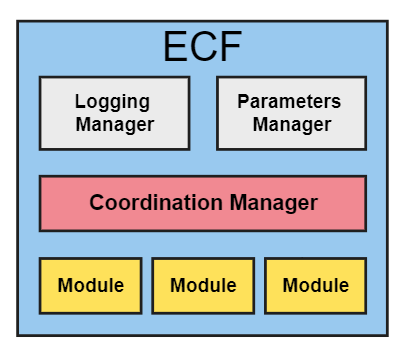
\includegraphics[width=0.5\textwidth]{ecf/ecf_structure}
    \caption{Extended Crazyflie component structure.}\label{fig:ecf_structure}
\end{SCfigure}

\section{The ECF Setup Process}\label{sec:ecf_setup_process}

The successful implementation of the facade design pattern allows for a centralized interface, accomplishing the second objective previously stated.
Still, the Extended Crazyflie does not include any automation processes, allowing users to eliminate the expensive setup phase and lowering the learning curve.

To understand how the ECF accomplishes this other objective, we need to take it a step further and analyze better how the structure described above is created when a new instance of the ECF is created.
In Figure~\ref{fig:ecf_sequence}, we can see the sequence of the operations performed at the component's initialization.
The ECF is directly linked to a Crazyflie 2.1, so before getting an instance of the main component, we need to know the address (uri) of the Crazyflie that we desire to connect.

The first thing the component does is to initialize the communication protocol drivers from the ground station to the drone and instantiate the connection between the two.
After establishing the connection, the ECF creates and initializes a unique instance for the Communication and Coordination Frameworks and stores them in its local storage.

To initialize the software sensing used for estimating its state (see Section~\ref{sec:state_estimate_and_control}) with a clean initial state, resetting the estimator before taking off is usually helpful. 
This process avoids that the state estimated in the previous flights influences the current run. 
The ECF uses the newly created Communication Framework to effectively reset the estimator by updating Crazyflie's state values relative to the estimated state.

The last operation in the initialization phase is the creation of the additional ECF Modules.
Since the module creation process is automatic and depends on the current configuration of decks onboard, the ECF needs to know this information.
To get the current configuration, it simply reads it through the Communication Framework.

Each module can be viewed as a simple component, so for each module needed, the ECF creates a new instance of the module's component and stores it in its local storage. 
The ECF stores its modules in a local repository so that each module's instance can be retrieved straightforwardly by accessing this repository.
For example, if a developer wants to use their drone that is mounting a Multiranger Deck and a FlowDeck; 
by simply initializing the ECF component, they will be able to communicate using the Communication Framework, execute actions at the right moment using the Coordination Framework, and access the features of the decks mounted with the Multiranger and FlowDeck module stored in the local repository.

This automatic setup process is of fundamental importance to facilitate the task of developers who use EasyFly.

\begin{figure}[tb]
    \centering
    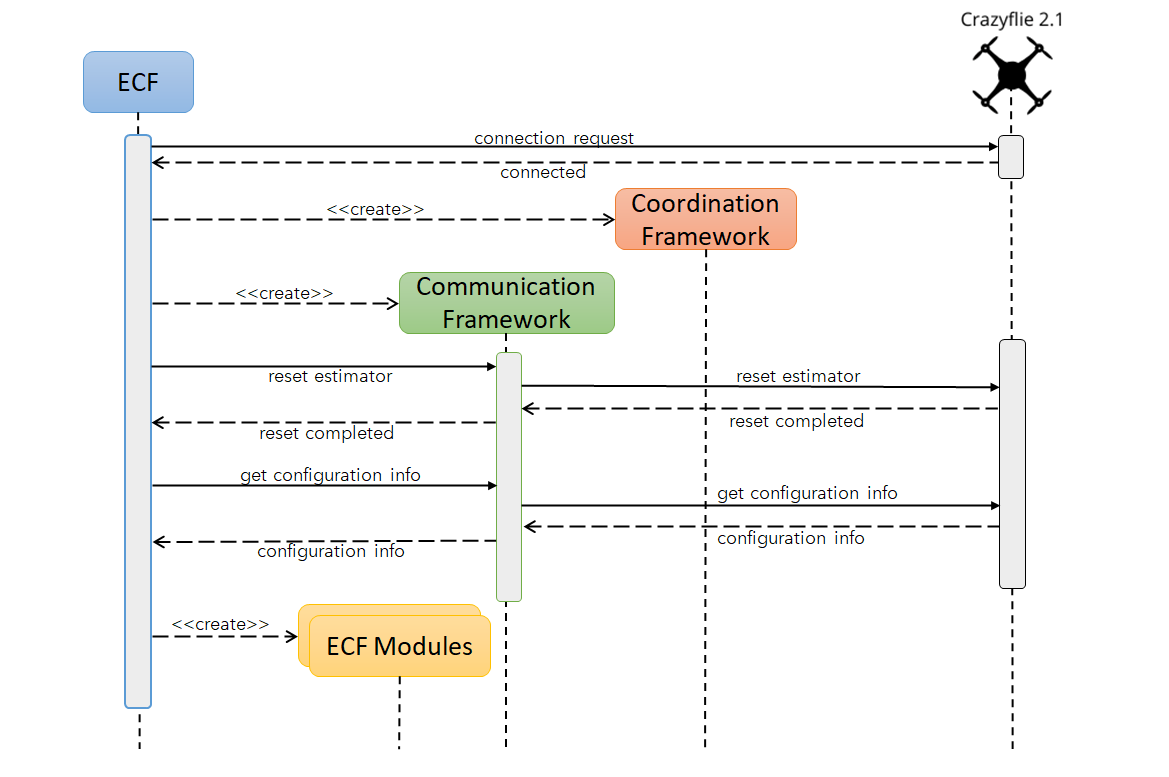
\includegraphics[width=0.9\textwidth]{ecf/ecf_sequence} 
    \caption[ECF initialization sequence diagram]{The sequence diagram of the setup process of the Extended Crazyflie shows the operations performed to have a working instance of the component}\label{fig:ecf_sequence}
\end{figure}

%% TODO MOVE to chapter 7

% \subsection{Extended Crazyflie Modules}\label{subsec:ecf_modules_overview}
% As we have seen, the Extended Crazyflie component instantiates a set of modules, each of which can be viewed as a container of functionality.
% So far, it is still unclear what such modules are, what their structure is, what those added functionality are, and last but not least, which type of modules the EasyFly programming environments have. 

% In this section, we will deeply understand ECF Modules, and we will answer all of these questions.
% Before entering into the details of modules, let's step back and understand the origin of the idea behind those modules.
% To make this, think back to the use case scenario solved in Section~\ref{subsec:coordination_manager}, and more generally, think of the process we proposed to develop a drone application easily using EasyFly.

% The steps that we followed were:
% \begin{itemize}
%     \item Define the state of the application
%     \item Setup the Coordination Framework to handle that state
%     \item Setup the Logging Manager to update correctly that state
%     \item Define how and when reacting to state changes
% \end{itemize}

% Apart from the first step, which is usually the most complex and depends mostly on the application scenario, we can say that the other steps are made of identical operations, almost independently from the application.
% Apparently, the first step, which defines the state, is indeed profoundly diverse across different applications.
% But if we analyze the possible states that the application can use, we can notice that the state is usually composed only of internal and sensed data; 
% resulting in a very limited set of variables.
% Ultimately, we will use the same state or a union of “standard” parts for most of the applications. 

% For example, the estimated position information is always crucial in almost any drone application. 
% Hence, we could define a component that automatically creates a state inside the Coordination Manager and keep it updated.

% An ECF Module is a component that defines a \textit{standard state}.
% Using the Communication and Coordination frameworks, it updates this state and makes it available through a \textit{standard Observable} inside the Coordination framework.

% By using standard modules, we reduced and focused (for most of the application) the development process to a single task: defining how and when reacting to state changes.
% The structure of an ECF module is shown in Figure~\ref{fig:ecf_module_structure}: it has a list of state variables, each of which is continuously updated every time a new value is available. 
% So, at any point, these variables contain the last value known read from the Crazyflie for that variable.

% As the last fundamental component, the ECF Module can include some utility functions strictly related to the state they define. 
% In the next chapter (see Chapter~\ref{ch:modules}), we will better analyze ECF modules and their utility functions.

% \sidecaptionvpos{figure}{c}
% \begin{SCfigure}[\sidecaptionrelwidth][tb]
%     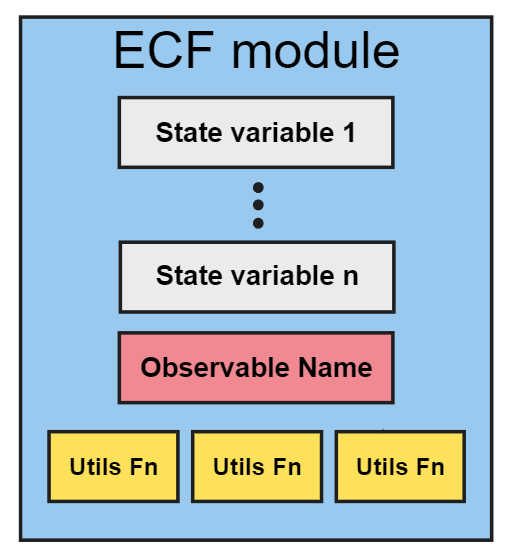
\includegraphics[width=0.5\textwidth]{ecf/ecf_module}
%     \caption{Extended Crazyflie Module internal structure.}\label{fig:ecf_module_structure}
% \end{SCfigure}

% To answer the last question: what type of ECF Modules exist in EasyFly? 
% We need to consider valuable states to become \textit{standard states}.

% Since our state can be defined either by internal state or by external sensed data, we decided to create the following Modules:
% \begin{itemize}
%     \item Internal State
%     \begin{itemize}
%         \item State Estimate Module
%         \item Battery Module
%     \end{itemize}
    
%     \item Sensed Data State
%     \begin{itemize}
%         \item Multiranger Module
%         \item Height Module
%         \item Lighthouse Module
%         \item Ai Deck Module
%     \end{itemize}
% \end{itemize}


% \subsection{Use Case Scenario's Solution}\label{subsec:solution_use_case_scenario}

% We analyzed in detail what ECF is and what its structure is. 
% Moreover, we described the purpose and the functioning of its core part, the ECF Modules. 

% At this point, we will show a possible solution to the same use case scenario we solved in Chapter~\ref{subsec:coordination_manager}, this time using the functionality of the ECF component.
% We purposely selected the same example that is already solved to see how much complexity the ECF handles, hiding it from the developer.

% For simplicity, we rewrite the specification of the example:
% \begin{displayquote}
%     For the drone application that we are developing, we need the drone to be maintained not too close to the walls of the flight area. 
%     Specifically, it must maintain a safe distance of 0,5 meters from the walls.
% \end{displayquote}

% If we analyze the requirements, we can say that the only information we need to know to control the drone is the distance from the wall. 
% For that purpose, we can use the Multiranger deck, which will give us the distance from the nearest obstacle in the four directions (see Section~\ref{deck:multi_ranger}).
% Before going straight forward to the implementation, we should briefly introduce the module that we will use in this example: the Multiranger module.
% The Multiranger module is an ECF module which defines a Sensed Data State as follows:
 
% \begin{lstlisting}[language=Python]
%     State = {
%         "left": "Distance from nearest obstacle on the left",
%         "right": "Distance from nearest obstacle on the right",
%         "front": "Distance from nearest obstacle on the front",
%         "back": "Distance from nearest obstacle on the back",
%         "up": "Distance from nearest obstacle above"
%     }
% \end{lstlisting}

% For this state, the Multiranger Module will create and keep updated an observable in the Coordination Manager. 
% We can take advantage of this Observable and subscribe to it to react when the distance goes below 0.5 meters.
% Here is the code of the example:

% \begin{lstlisting}[language=Python]
% from cflib.positioning.motion_commander import MotionCommander
% from extension.decks.deck import DeckType
% from extension.extended_crazyflie import ExtendedCrazyFlie

% def safe_distance(multiranger_state : dict, mc : MotionCommander):
%     if multiranger_state['left'] < 0.5:
%         mc.right(0.5 - multiranger_state['left'])
%     if multiranger_state['right'] < 0.5:
%         mc.left(0.5 - multiranger_state['right'])
%     if multiranger_state['front'] < 0.5:
%         mc.back(0.5 - multiranger_state['front'])
%     if multiranger_state['back'] < 0.5:
%         mc.forward(0.5 - multiranger_state['back'])
    
% with ExtendedCrazyFlie('radio://0/80/2M/E7E7E7E7E7') as ecf:
%     with MotionCommander(ecf.cf) as mc:
%         ecf.coordination_manager.observe(
%         	observable_name= ecf.decks[DeckType.bcMultiranger]
%                                 .observable_name,
%         	action= safe_distance,
%             context= [mc],
%         )
% \end{lstlisting}

% The code is organized into two main parts; the first part (\textit{lines 6-14}) is a function that contains the core logic of the application. 
% If we analyze the signature, the function is an Action of the Coordination Framework: it takes as input the state of one observable and a MotionCommander object (the context) that is used to act on the Crazyflie effectively.

% Four \textit{if} statements in the function's body check whether the distance from the nearest obstacle in one direction is below 0.5 meters. 
% If that is the case, the function will use the Motion Commander object to move the drone in the opposite direction, bringing the drone back to a safe distance from the obstacle.

% The second part (\textit{lines 17-23}) instead represents the only setup needed to create a working application. 
% It comprises 2 \textit{with} statements and a single function call. 

% Line 17 will create a new instance of Extended CrazyFlie and assign it to the variable \textit{ecf}.
% As we know, all the setup operations are performed by creating the ECF component. 
% Since we are mounting a Multiranger deck, it will also automatically create an instance of the Multiranger Module. 
% The user with a single line of code is ready to use all its functionality. 

% Line 18 will create and initialize an instance of the Motion Commander. 
% The Motion Commander is a functionality offered by the base cflib (see Section~\ref{sec:flight_control}), which exposes some functionality that allow controlling the drone flight. 

% In line 19, there is a call to the Coordination Manager to set up a subscription to the multiranger observable. 
% In particular, we specified an action, the \textit{safe\_distance} function, and a context, the Motion Commander's instance \textit{mc}. 
% In this way, every time the Multiranger Module updates the state, the \textit{safe\_distance} function will be called with the new state and the instance of the Motion Commander; if the function finds anomalies in the distance, it will apply a correction.

% As we can see, the resulting code is clean and easy to understand, and all the complicated setup operations are handled automatically under the hood.
% The Extended CrazyFlie component is a tool with much potential that allows the developer to start with the proper setup by writing a single line of code. 
% Moreover, with standard ECF Modules, the developer can focus on the application's core business logic and reduce the skills needed to program an application and the time necessary to complete it effectively. 

\chapter{Communication Framework}
\label{ch:communication}
In the domain of drone systems, effective communication stands as a central pillar for operational success.
Communication with drones refers to the process of transmitting and receiving information between a drone and a remote control device or computer system. 
It involves the use of various technologies, including Wi-Fi, Bluetooth, and radio frequency (RF) signals, to control the drone and receive real-time data and feedback.

This chapter focuses on a crucial element of our drone programming environment: the Communication Framework. 
Its purpose is to handle all the communication between the ground station and the flying drone. 
More in detail, the Communication Framework is a software component hosted on the ground station 
that allows the user to establish effective communication between the script running on the ground station and the drone.

The Communication Framework manages the communication stream into two separate flows: parameter setting and telemetry logging.
The former is the flow of communication that is directed from the ground station to the drone; it is used to set configuration parameters onboard the drone.
The latter is the opposite flow of communication, from the drone to the ground station, and it is used to receive all the telemetry data of the drone, allowing for better control.


\section{The Communication Infrastructure}\label{sec:communication_infrastructure}
Before diving into the details of our Communication Framework, it is crucial to understand the underlying communication infrastructure. 

As described in Chapter~\ref{ch:tools}, our programming environment is spread into two main devices: the ground station and the drone.
The drone's firmware is written in C++ and runs on a small board with limited resources. On the other side, the ground station runs Python scripts
that control the drone's behavior. The heterogeneity between these two subsystems increases the complexity of the communication process.

The platform uses a custom network protocol called CRTP to overcome all these challenges. 
CRTP was designed to allow packet prioritization to help real-time control of the Crazyflie; in the current implementation, the link guarantees strict packet ordering within a port.

As shown in figure~\ref{fig:communication_stack}, the Crayzyflie communication is implemented as a stack of independent layers.
Every layer of the communication stack has two parallel implementations, one hosted in the firmware onboard and the other on the ground station's software.

The physical layer is responsible for transmitting packets to and from the Crazyflie. 

The link implements safe and ordered packet channels to and from the Crazyflie. This layer abstracts the physical medium and implements one transmitting and receiving packet channel to and from the Crazyflie.

The CRTP layer introduces the concept of a logical packet; each packet measures 32 Bytes and is composed of three parts: port, channel, and payload.
The tuple \textit{port:channel} allows the packet to be delivered to the specialized subsystem that receives and processes the message.

\sidecaptionvpos{figure}{c}
\begin{SCfigure}[\sidecaptionrelwidth][tb]
    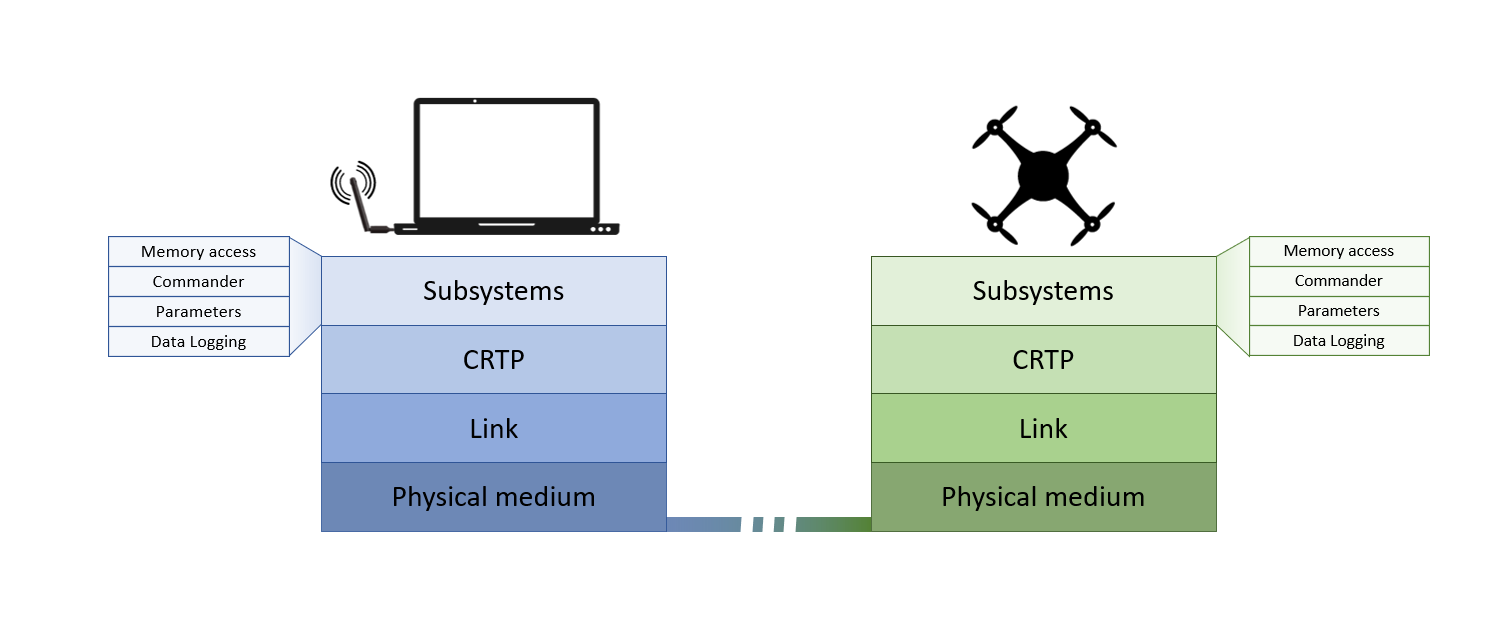
\includegraphics[width=0.5\textwidth]{communication/communication_stack}
    \caption[The Crazyflie communication stack]{The Crayzyflie communication stack is composed of 4 independent layers: Subsystems, CRTP, Link, Physical medium}
    \label{fig:communication_stack}
\end{SCfigure}

In the higher-order layer, we can identify four principal subsystems:
\begin{itemize}
    \item \textbf{Memory access} -- that manages memory operation on the Crazyflie's physical memories, e.g., trajectory uploading.
    \item \textbf{Commander} -- that send/receive control set-points.
    \item \textbf{Parameters} -- that manages read/write operations on configuration parameters of the Crazyflie.
    \item \textbf{Data Logging} -- that handles logs of telemetry data sent periodically from the Crazyflie to the ground station. 
\end{itemize} 

The first two subsystems (memory access and commander) are the simplest, with a straightforward implementation. 
They expose some methods through an API, and when called, they craft a packet, fill it with parameters data, and send it to the link layer.
On the other side, the same subsystem receives the packet, unpacks the data, and executes the desired function.

Conversely, the parameters and data logging subsystems have some peculiarities that make them more complex. 
In particular, the parameters subsystem allows performing read/write operations with acknowledgments of the successful operation.
The data logging subsystem, instead, must support periodical updates of telemetry data.
Moreover, both the two subsystems must handle a variety of variables with different types.

The Communication Framework that we designed and developed is meant to wrap the functionalities of these two complex subsystems and offer the user a more usable and efficient way to handle data logging and parameters.


\section{The Design of the Communication Framework}\label{sec:communication_frameworks_design}

The Communication Framework is a software component that provides an easy and accessible way to set parameters onboard the Crazyflie and to log telemetry data.
This component is part of the ground station's software and has been designed as a publish/subscribe system.

Every CRTP data that is routed to the parameter or logging subsystem is managed by the Communication Framework and stored in a central repository.
Every other software component or script interested in such data can use the Communication Framework to access the repository and subscribe for value updates.

Given the profound semantic difference between the logging and parameters subsystems, we decided to keep the two concepts separated inside the Communication Framework.
For this reason, we developed two different Communication Managers, one for every subsystem. The two implementations, namely the Logging and the Parameters Manager, 
shares the publish/subscribe design structure, but they slightly differ in the management of the updates in the repository.

\subsection{The Logging Manager}\label{subsec:logging_manager}

As described above, the Logging Manager is one of the two implementations of the Communication Framework. 
In particular, the role of the Logging Manager is to handle the setup and the periodic updates of telemetry data sent from the Crayzyflie.

The internal structure of this component is represented by a values repository where key-value pairs are stored to maintain the telemetry state.
More in detail, each variable, identified by a unique key, represents an entry inside the values repository; the value of the entry is the last updated value of the logged variable.

In a separate repository, the Logging Manager stores the subscribers interested in the variables updates. 
In this second repository, the component stores a list of references to subscribers for each single variable or set of variables. 
Each reference consists of a predicate function to allow filtering updates and a callback function to effectively notify the subscriber when the predicate is satisfied with the new value.

To better understand the working principle behind the Logging Manager, we illustrated the complete workflow in Figure~\ref{fig:logging_manager}.

Whenever the script running on the ground stations needs to start tracking a variable, the Logging Manager creates or updates a log configuration and sends it to the Crazyflie.
The configuration contains information regarding the variable name, the type, and the desired period of updates. 

At some point, when the script is interested in reading and getting updated on the variable's values, it creates a callback function, i.e., an action to be executed with the new updated value, and, optionally, a predicate function for receiving updates only when the values satisfy certain constraints.

Then, the script registers these functions to the Logging Manager, specifying the single variable or set of variables of interest.
When the logging process starts, the Crazyflie sends periodic messages containing the variable updates; the Logging Manager intercepts those messages and updates its internal values repository.
Each time an update occurs, the Logging Manager checks whether any subscriber is watching that variable. 
If so, for each subscriber, it evaluates the predicate and eventually notifies the subscriber by calling the registered callback. 

\begin{figure}[tb]
    \centering
    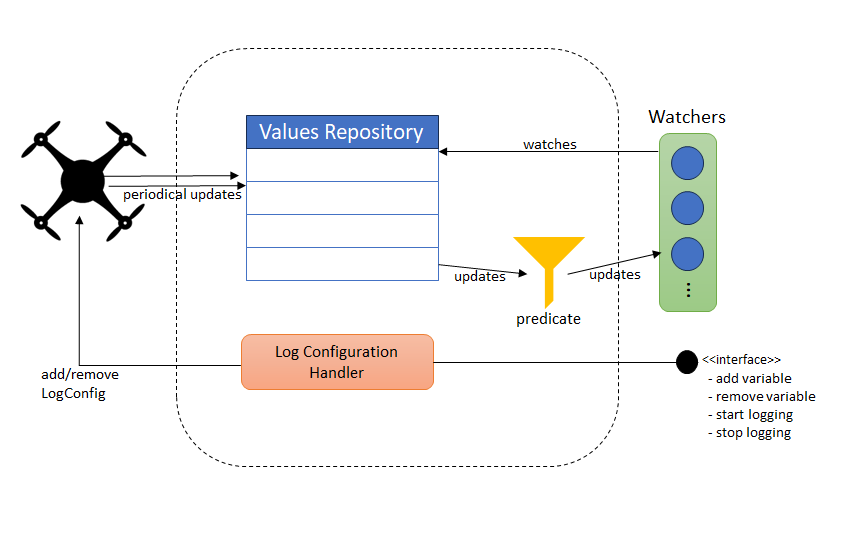
\includegraphics[width=0.9\textwidth]{communication/logging_manager}
    \caption{Logging Manager's workflows.}\label{fig:logging_manager}
\end{figure}

Given that each variable can have its own size (given the type) and period, the Logging Manager needs to handle different log configurations.
Moreover, the single configuration has a size constraint of 26 Bytes given by the size of the CRTP packet, increasing the complexity of the configuration management.

To optimize the number of log configurations created, each time the Logging Manager needs to add a variable, 
it searches for a suitable existing configuration with enough space to fit it. 
The Logging Manager only adds a new configuration when strictly necessary, ensuring maximum optimization.

\subsection{The Parameters Manager}\label{subsec:parameter_manager}

The other implementation of the Communication Framework, the Parameters Manager, manages the configuration operations of the Crayzyflie.
The Crayzyflie 2.1 allows the users to set parameter values to configure the desired setup. 
An example of a parameter could be the selected state estimator, i.e., Extended Kalman Filter or Complementary Filter (See Section~\ref{sec:state_estimate_and_control}).

Following the same structure as the Logging Manager, also the Parameters Manager has one value and one subscriber repository where it stores, respectively, the current value for tracked parameters and the references of subscrbers for each variable.

Conversely, variable updates are managed slightly differently with respect to the Logging Manager. 
In fact, the underlying parameters subsystem does not have a periodic update of values; instead, the updates happen only when the parameter's value is effectively changed onboard.
In other words, the Parameters Manager only receives and processes an update when the Crazyflie acknowledges a state change in the parameter's value.
 
Figure~\ref{fig:parameters_manager} represents the operations workflow inside the Parameters Manager. When needed, usually before the takeoff,
the script can use the Parameters Manager to read or write configuration values. 

Read operations are processed straightforwardly with a synchronous request-response messages exchange. 
The request contains the name of the variable, and the Crazyflie's response contains the current value of the requested parameter.

Write operations, on the other side, are processed asynchronously; first, a request message is sent from the Parameters Manager to the Crazyflie,
then, when the Crayzyflie successfully completes the update, it notifies the ground station's Parameters Manager.

Once the Parameters Manager receives a value, it uses the internal publish/subscribe system to notify subscribers.  

\begin{figure}[tb]
    \centering
    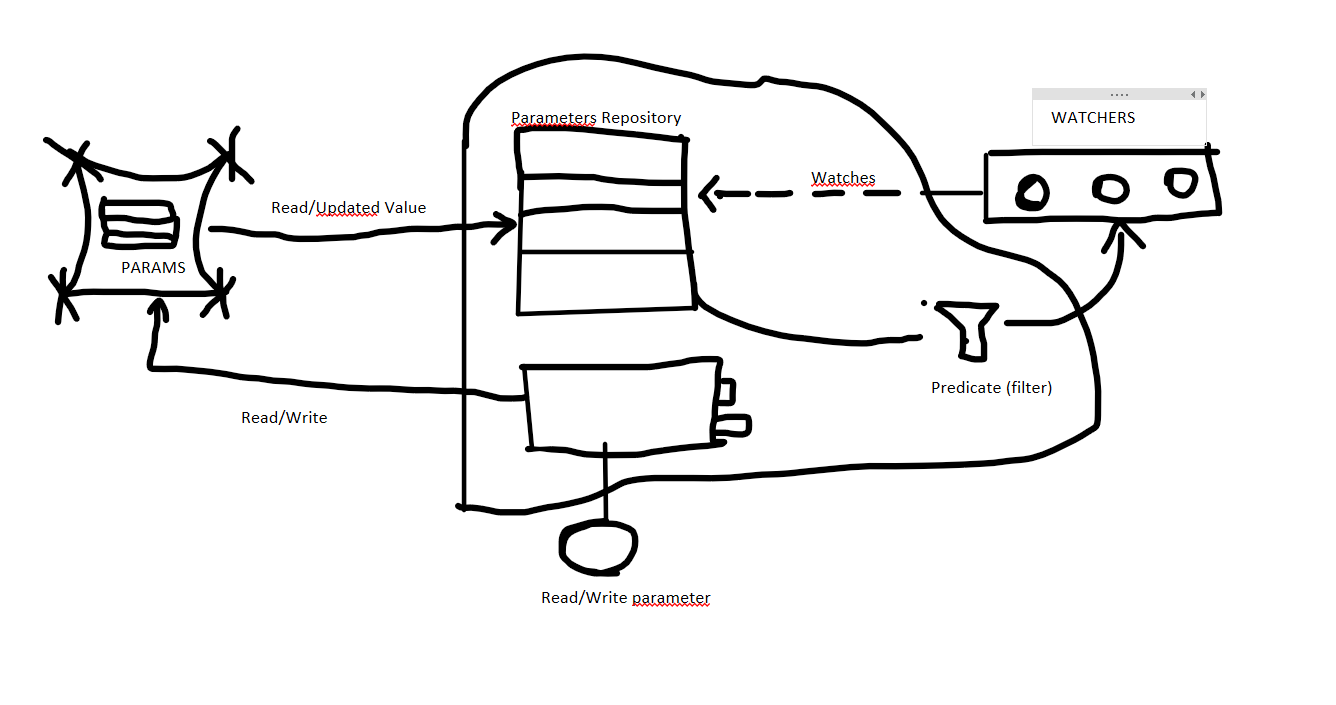
\includegraphics[width=0.9\textwidth]{communication/parameters_manager}
    \caption{Parameters Manager's workflows.}\label{fig:parameters_manager}
\end{figure}



\chapter{Coordination Framework}
\label{ch:coordination}
In any drone application, the drone's ability to react after an event is a key factor for the success of the application itself. 
In this chapter, we present EasyFly's Coordination Framework, a software component belonging to the ground station system meant to coordinate and orchestrate all the actions of the Crazyflie. 

The Coordination Framework acts as a centralized entity that is able to synchronize different parts of the same applications.
Moreover, it is possible to coordinate multi-drone applications easily using the Coordination Framework.

In this chapter, we first present the role of this framework and its use cases, providing some concrete examples of possible applications. 
Then, we will analyze its structure and design principle in detail.


\section{The Role of the Coordination Framework}\label{sec:coordination_framework_rolw}

Coordination plays a crucial role in the successful implementation of drone applications. 
Depending on the application type, the coordination of a drone can be seen at two different levels:
\begin{itemize}
    \item Intra-drone coordination
    \item Inter-drone coordination
\end{itemize}

The first level of coordination considers the drone as an individual. 
In this case, coordination is considered to be the process of reacting in the face of a change in the surrounding environment or the drone's internal state with an ad hoc action properly defined.

In the case of intra-drone coordination, the role of the Coordination Framework is to watch over the current state of the drone (internal state or sensor data). 
When a specific condition is met, it performs the corresponding action.

A simple use case of the Coordination Framework considering intra-drone communication can be represented by the following:

\begin{displayquote}
    For the drone application that we are developing, we need the drone to be maintained not too close to the walls of the flight area. 
    Specifically, it must maintain a safe distance of 0,5 meters from the walls.
\end{displayquote}

In the use case scenario described above, the Coordination Framework will act as a supervisor entity that watches the values read from the lateral proximity sensors of the drone. 
Whenever the distance is less than or equal to 0,5 meters, it will dispatch the action to move the drone in the opposite direction, bringing the distance from the wall back over the safe distance required.

Conversely, inter-drone coordination applies only to applications where the number of drones is more than one.
In these cases, the coordination is considered among individuals belonging to the same swarm.

By synchronizing the actions of multiple drones, coordination allows for the efficient and effective achievement of complex tasks that would be difficult or impossible for a single drone to accomplish alone. 
In this type of application, the role of the Coordination Framework is to watch over the state of the entire swarm and perform actions whenever a condition on the swarm state is met.

To make this concept of inter-drone coordination clearer, let's consider also in this case a simple use case:

\begin{displayquote}
    We need to develop a swarm drone application that performs simple choreography for a demonstration during a fashion event. 
    Our swarm is composed of three drones: D1, D2 and D3. 
    The choreographer designed the choreography: D1 starts flying and slowly increases its height to 1 meter from the ground. 
    After D1 completes its movement, D2 also starts flying and reaches a height of 0.5 meters. 
    When D2 has reached the target height of 0.5 meters, the drones D1 and D3 will slowly meet D2 at 0.5 meters from the ground. 
    Finally, to complete the choreography, land all the drones together.
\end{displayquote}

In this use case scenario, the Coordination Framework needs to track the height of each swarm component.
For this reason, the swarm state will be represented by the tuple \(\langle D1~altitude, D2~altitude, D3~altitude \rangle\). 
Whenever the state changes, the Coordination Framework will decide on which actions to take according to the Table~\ref{table:inter_drone_use_case}

\begin{table}[H]
    \centering
        \begin{tabular}{*{4}{|c}|}
        \hline
        \rowcolor{bluepoli!40}
        \textbf{D1 altitude} & \textbf{D2 altitude} & \textbf{D3 altitude} & \textbf{Action to take } \\
        \hline \hline
        0 & 0 & 0 & move D1 up to 1 meter \\
        \hline
        1 & 0 & 0 & move D2 up to 0.5 meter \\
        \hline
        1 & 0.5 & 0 & move D1 down and D3 up to 0,5 meter \\
        \hline
        0.5 & 0.5 & 0.5 & land all the drones \\
        \hline
        \end{tabular}
        \\[10pt]
        \caption{Use case scenario of inter-drone communication.}\label{table:inter_drone_use_case}
    \end{table}
    
The key advantage of using this approach in both intra and inter-drone communication is that the entire business logic of the application is defined inside the Coordination Framework.
This fact implies that the only challenging task that the developer needs to take care of is the definition of the state and the relative actions to take when the state changes.
If the state is correctly updated and some external entity properly performs the actions defined, the Coordination Framework will orchestrate all the stuff to achieve the application's goals correctly.

\section{Structure and Design Principles}\label{sec:coordination_structure_design}

The design structure of the Coordination Framework is a publish-subscribe architecture that follows the principle of the observer pattern.

The observer pattern is a design pattern in software engineering that defines a one-to-many relationship between entities,
where changes in one entity (the `observable` or `subject`) are automatically propagated to other entities (the `observers`) that depend on it.

In the observer pattern, the observable stores a list of observers and notifies them automatically whenever it changes state. 
This way, observers can take action based on the observable's new state without constantly polling it for changes.

Following this design pattern, we designed the Coordination Manager considering four main actors:
\begin{itemize}
    \item \textit{Observable} -- Represents a state that can change over time.  
    
    \item \textit{Producer} -- The script/component that creates the Observable, providing an initial state. 
    Usually, this actor is in charge of updating the state of the Observable during time.

    \item \textit{Observer} -- The script/component interested in watching some Observables' changes. 
    Upon subscribing to the Observable, the Observer is notified by the framework when the former's state changes.

    \item \textit{Coordination Manager} -- It is the component in charge of managing the entire state of the drone application, allowing Producers to update the value of a portion of the state and notifying Observers whenever this happens.
\end{itemize}


\begin{figure}[h]
    \centering
    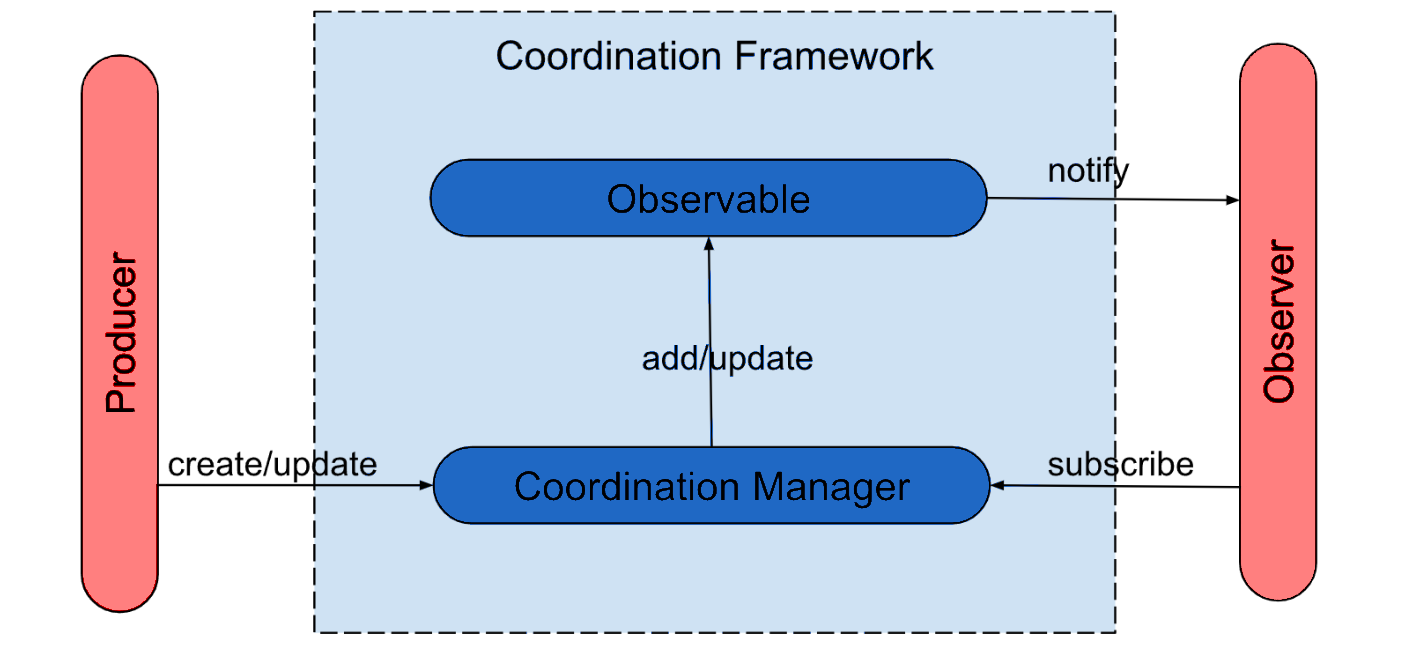
\includegraphics[width=0.9\textwidth]{coordination/design_architecture}
    \caption[The architecture of the Coordination Framework]{The architecture of the Coordination Manager comprises two internal entities: the Observable and the Coordination Manager. 
    Conversely, Producers and Observers are external to the framework and interact with it. }\label{fig:coordination_design_architecture}
\end{figure}

As presented in Figure~\ref{fig:coordination_design_architecture}, the core of the Coordination Framework is composed only of the Observable and the Coordination Manager entities.
The Producer and the Observer are entities considered outside the frameworks and only act as utilizers of its functionalities.

\subsection{The Observable}\label{subsec:observable}
In our Coordination Framework, the Observable can be considered as the basic block of the entire structure.
In the core, the Observable holds a piece of information known as the state of the Observable. 

The state can be as complex as desired, and most importantly, it can change over time. 
Moreover, the state is atomic and cannot change partially; in other words, regardless of the complexity of the state, every update must provide complete information.

The Observable, on its own, is meaningless. 
It becomes valid only when an external entity (observer) is interested in watching the state and being notified when some update occurs.

For this reason, the Observable stores a list of references, known as subscriptions, to the external entities interested in watching the value of the state. 
In the standard observer pattern, the subscription consists of a callback function that the Observable uses to notify the Observer of the new value.
In our implementation, we decided to add some additional information to the subscription to increase the functionality of the pattern.
In particular, the subscription is a tuple composed of the following parts:
\begin{itemize}
    \item \textit{Action} -- A callback function to be called whenever the state of the Observable changes
    \item \textit{Condition} -- A predicate function that filters the values before notification. It is a function of the updated state of the Observable and decides whether to notify the Observer or not. 
    \item \textit{Context} --  It is an optional object to be passed as a parameter to the Action. It can contain some helpful information to allow the Observer to take the action. 
    When subscribing, the Observer can provide an arbitrary Context value; the provided Context will be stored in the subscription and sent back with each notification.
\end{itemize}

In the current implementations of the Coordination Framework, we have developed two types of Subsctipions, one synchronous and the other asynchronous. 
As the names suggest, the synchronous subscription will block the execution of the Observer until the state is updated and the condition is satisfied.
Conversely, using the asynchronous subscription, the Observer will continue executing and be called back later when the value changes and the condition is met.

The standard observer pattern provides only the asynchronous notification. 
We decided to extend the pattern with the synchronous one also because, sometimes, it is useful to check that the drone application is in the desired state before continuing the execution.

\subsection{The Coordination Manager}\label{subsec:coordination_manager}

The Coordination Manager is the orchestrator of the entire Coordination Framework. 
Its role is to manage the whole application's Observables, creating and updating them when requested by some external Producer.

Its core is a global repository of Observables, representing the whole application state. 
Inside this repository, the Observables are identified by a unique name. 

As shown in Figure~\ref{fig:coordination_design_architecture}, the Coordination Manager represents the facade of the entire Coordination Framework; external entities like Producers and Observers are forbidden to manipulate the values stored inside the Observables directly.
This constraint allows centralized control, avoiding any possibility of an inconsistent state.

To better understand the working principle of the Coordination Framework, we can show in action the Coordination Manager explaining more in detail how the use case scenario described at the beginning of the chapter can be easily solved with this approach.

The scenario is the following:
\begin{displayquote}
    For the drone application that we are developing, we need the drone to be maintained not too close to the walls of the flight area. 
    Specifically, it must maintain a safe distance of 0,5 meters from the walls.
\end{displayquote}

The first thing to do to solve this problem using the Coordination Manager is to define the State of the application. 
In particular, we can identify four Observables:
\begin{itemize}
    \item \textsc{Left Observable} 
    \item \textsc{Right Observable} 
    \item \textsc{Front Observable} 
    \item \textsc{Back Observable}
\end{itemize}

Our state is then represented by the following:

\begin{lstlisting}[language=Python]
State = {
    "Observable_Left": "Distance from Left wall",
    "Observable_Rigth": "Distance from Right wall",
    "Observable_Front": "Distance from Front wall",
    "Observable_Back": "Distance from Back wall",
}
\end{lstlisting}


Once we have defined the state and managed the update of such a state, then we can define the second part of the Coordination Manager.
To do this, we can set up 4 Observers, one for each Observable, to move the drone away from the respective wall.
In particular, for each Observer, we can define an Action like the following:

\begin{lstlisting}[language=Python]
def move_away_left_wall_action( actual_distance, contex):
	context.move_drone_right(0.5 - actual_distance)

def move_away_rigth_wall_action( actual_distance, contex):
	context.move_drone_left(0.5 - actual_distance)

def move_away_front_wall_action( actual_distance, contex):
	context.move_drone_back(0.5 - actual_distance)

def move_away_back_wall_action( actual_distance, contex):
	context.move_drone_front(0.5 - actual_distance)
\end{lstlisting}

Moreover, since we want to perform the action only if the distance from one wall is less than 0.5 meters, we can specify for all the Observer the following Condition function:

\begin{lstlisting}[language=Python]
def closer_enough_condition(actual_distance):
	return actual_distance < 0.5
\end{lstlisting}

With this approach, the main advantage is that the entire business logic of the application is defined inside the Coordination Framework.
As the solution to the use case shows, this framework simplifies the task for a user, letting them focus on the definition of state and reactions instead of trying to manage all the coordination between the parts. 

Another advantage is that the resulting code is clean and can easily be read and understood also by users with less programming experience.

On the other hand, when the number of Observables and Observers starts to become very big, the constraint of handling everything in a single and centralized component will surely introduce some overhead.


\chapter{ECF Modules}
\label{ch:modules}
In Chapter 4~\ref{ch:ecf}, we briefly introduced ECF Modules, describing them as an encapsulated set of functionality operating on a specific programming environment feature.
Since this point, we have treated them as helpful back boxes without profoundly understanding their concrete design.

In this chapter, we will analyze each ECF Module available in the EasyFly extension in detail, describing the purpose, main functionality, and implementation details for each. 
First, We will give an overview of the concept behind the ECF Modules, understanding the motivations and principles that make these modules the most essential part of the EasyFly programming environment.
Then, we will enter in the detail of each ECF Module implemented, providing the specific utility and use cases.

\section{ECF Modules Overview}\label{sec:modules_overview}
For a programming environment like EasyFly that is meant to be used for HDI research, the system's modularity is a key feature that cannot be missed.
In fact, a modular system allows the configuration to adapt to any possible change in the surrounding environment or the application's requirements.

As we have seen in the final example of the previous chapter (see Listing~\ref{example_coordination}), the resulting code is still full of repetitive operations that make the code less clear and prone to errors.
For this reason, our EasyFly programming environment is still missing a lot of automatic processes that can help reduce developers' effort and increase usability. 

\pagebreak% REASON FORMAT 

If we look in detail at the process adopted to solve the previous chapter's example, we can identify four main steps:
\begin{enumerate}
    \item Define the state of the application and \( \langle Event, Condition, Action \rangle \) tuples
    \item Setup the Coordination Framework to handle that state
    \item Setup the Logging Manager to update correctly that state
    \item Define how and when reacting to state changes
\end{enumerate}

Given the fact that almost any drone application can be modeled using\\
\( \langle Event, Condition, Action \rangle \) tuples, we can undoubtedly apply the above solution methodology for all such applications.
Moreover, we can say that the process's most challenging and application-related part is the first step; the other parts are straightforward.

Since the possible states of an application depend mainly on the basic information that the platform provides, like telemetry data, we can automatize the setup process (points 2 and 3) for the basic information.
For example, since most of the applications will use the estimated position of the Crazyflie, we can create a \textit{standard state} containing position-estimated information and maintain it updated using the Coordination Framework.

In this way, every developer who needs estimated position information can access this standard state and use the information as required.

The ECF Modules are the software components that implement the automatic process of updating standard states. Moreover, they add the modularity feature to our programming environment.

Sometimes, the simple raw information is useless for a developer; therefore, the ECF Modules usually contain a set of functionality that allows the processing of the information cleverly. 


\section{State Estimate Module}\label{sec:module_state_estimate}
Regardless of the purpose, a crucial aspect of operating a drone is having a deep understanding of the drone's position, velocity, and acceleration. 
These parameters are vital for ensuring the drone's stability and safe navigation. 
Accurate knowledge of the drone's position and speed enables its operator to control its movements and avoid obstacles or hazards in its path. 
Furthermore, understanding acceleration is crucial in achieving precision and accurate control of the drone's movements.
State estimate accuracy depends on how much information the control loop can use. 
In particular, the decks that contribute more to the estimation process are the Lighthouse positioning Deck and the Flow Deck V2. 

As the name suggests, the State Estimate Module is an ECF Module that manages the estimated variables of the Crazyflie 2.1.
The role of this module is to keep the information relative to the estimated variables inside the Coordination Framework updated.
In this way, a developer that needs this information finds them already in the Coordination Framework instead of losing time setting up the logging on their own.

The full state of the State Estimate ECF Module is detailed in Table~\ref{table:estimate_module_state}

\begin{table}[tb]
    \centering
    \begin{tabular}{*{2}{|c}|}
    \hline
    \rowcolor{bluepoli!40}
    \textbf{Variable} & \textbf{Description} \\
    \hline \hline
    x & Position on the x-axis from the origin \\
    \hline
    y & Position on the y-axis from the origin \\
    \hline
    z & Position on the z-axis from the origin \\
    \hline\hline
    vx & Velocity on the x-axis \\
    \hline
    vy & Velocity on the y-axis \\
    \hline
    vz & Velocity on the z-axis \\
    \hline\hline
    ax & Acceleration on the x-axis \\
    \hline
    ay & Acceleration on the y-axis \\
    \hline
    az & Acceleration on the z-axis \\
    \hline\hline
    roll & Roll in rad \\
    \hline
    pitch & Pitch in rad \\
    \hline
    yaw & Yaw in rad \\
    \hline\hline
    rateRoll & Roll rate in rad/s \\
    \hline
    ratePitch & Pitch rate in rad/s \\
    \hline
    rateYaw & Yaw rate in rad/s \\
    \hline
    \end{tabular}
    \\[10pt]
    \caption{ECF State Estimate Module's state.}\label{table:estimate_module_state}
\end{table}

Because the control loop onboard the Crazyflie 2.1 runs at 500Hz, a new estimation is computed every two milliseconds; these variables can rapidly change over time. 
We need to update the state as frequently as possible to ensure that the information provided is accurate and precise. 
For this reason, we selected the lowest possible sampling period for the Communication Framework, which is 10 milliseconds.

In this ECF Module, the utility functions allow the user to record the state variable and, at the end of the flight, plot the recorded data.
As with any other telemetry data, it is usually vital for a user to have the possibility to analyze that information after the flight, especially in the development phase of the application.
For this reason, the utility functions that we implemented will allow a user to analyze and compare data from multiple application runs.

\section{Battery Module}\label{sec:module_battery}

When dealing with drones, battery management is an important factor that must always be considered. 
Usually, due to its weight, the battery has minimal capacity, especially on drones with small dimensions.

An application can be perfectly developed, but it can easily fail if it does not consider the limitation of resources like the battery.
To help the developer with this task, we created another ECF Module that manages battery-related information and keeps them updated.

Given this, the full state of the Battery ECF Module is shown in Table~\ref{table:battery_module_state}


\begin{table}[tb]
    \centering
    \begin{tabular}{*{2}{|c}|}
    \hline
    \rowcolor{bluepoli!40}
    \textbf{Variable} & \textbf{Description} \\
    \hline \hline
    pm\_state & Battery power management state \\
    \hline
    voltage & Battery voltage in V \\
    \hline
    battery\_level & Estimated battery level in percentage \\
    \hline
    \end{tabular}
    \\[10pt]
    \caption{ECF Battery Module's state.}\label{table:battery_module_state}
\end{table}

The first variable of the state, \textit{pm\_state}, represents the state in which the power management of the drone is in.
The state can be one of the following:
\begin{itemize}
    \item Battery -- The drone is on and using its battery.
    \item Charging -- The drone is plugged into the power supply.
    \item Charged -- The drone has completed the recharge, and its battery is fully charged.
    \item Low Power -- The drone needs to be recharged.
\end{itemize}

With the other two properties of the state, \textit{voltage} and \textit{battery\_level}, the developer can determine with high precision the recharging phase.

Since battery management strictly depends on the application to be developed, it is hard to find an implementation that satisfies all the possible usage.
For this reason, the module is responsible only for keeping the information in the state consistent and updated.

\section{Multiranger Module}\label{sec:module_multiranger}

The Multiranger deck is an accessory board for the Crazyflie 2.1. 
The deck is designed to provide the drone with range-sensing capabilities, allowing it to detect objects and obstacles in its environment.

The Multiranger deck features four integrated ultrasonic sensors, which can be used to measure distances in a range of up to 4 meters. 
These sensors emit high-frequency sound waves that bounce off of nearby objects and return to the deck, allowing the deck to calculate the distance to the objects based on the time it takes for the sound waves to return.
Multiranger deck is a powerful tool for adding range sensing capabilities to the Crazyflie 2.1, enabling it to perform a range of applications such as mapping, autonomous navigation, and obstacle avoidance.

As with any other ECF Module, the Multiranger Module also has a state it manages. 
Table~\ref{table:multiranger_module_state} shows that the state is composed of the five range measurements, one for each direction it supports.


\begin{table}[tb]
    \centering
    \begin{tabular}{*{2}{|c}|}
    \hline
    \rowcolor{bluepoli!40}
    \textbf{Variable} & \textbf{Description} \\
    \hline \hline
    front & Distance from the nearest obstacle on the front (up to 4m) \\
    \hline
    back & Distance from the nearest obstacle on the back (up to 4m)\\
    \hline
    right & Distance from the nearest obstacle on the right (up to 4m) \\
    \hline
    left & Distance from the nearest obstacle on the left (up to 4m) \\
    \hline
    up & Distance from the nearest obstacle above (up to 4m) \\
    \hline
    \end{tabular}
    \\[10pt]
    \caption{ECF Multiranger Module's state.}\label{table:multiranger_module_state}
\end{table}

Given the wide range of applications the Multiranger deck fits, we decided to implement a simple implementation of two use cases of this deck directly inside the module:
\begin{itemize}
    \item Object Tracking 
    \item Obstacle Avoidance
\end{itemize}

With the Object Tracking behavior, the drone searches for an object to track when it starts. 
As soon it detects an object inside a configurable range, that object becomes the guide to follow. 
The drone with this behavior will try to follow whenever the tracked object moves in space. 

The velocity needs to change depending on the distance from the object. 
If the object is on the perimeter of the activation range, we need to move fast towards it, trying not to lose the tracking. 
On the other hand, when the object is closer to the safe range, the velocity can be slowed since the object is closer to the drone.
The drone uses the safe range to never hit the tracked object.

In summary, as we can see in Figure~\ref{fig:multiranger_tracking}, the drone with an Object Tracking behavior has two ranges:
The first range, which is the activation range, is used to determine what the tracked object is.
The second range, the safety range, is used to prevent collision with the tracked object when it stands at a fixed point.

\sidecaptionvpos{figure}{c}
\begin{SCfigure}[\sidecaptionrelwidth][tb]
    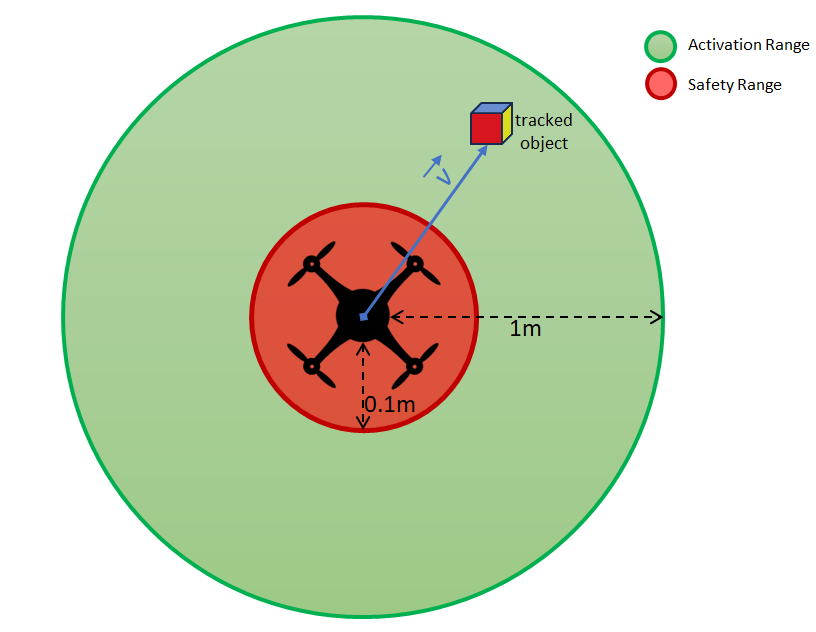
\includegraphics[width=0.5\textwidth]{modules/multiranger}
    \caption{Multiranger Object Tracking behavior.}\label{fig:multiranger_tracking}
\end{SCfigure}

The Obstacle Avoidance behavior is the opposite behavior with respect to object tracking. 
In this case, the activation range is used to determine an obstacle to fly away from.

When an obstacle is detected on the perimeter of the activation range, the drone will slowly start moving in the opposite direction. 
If the obstacle is dynamic and gets closer, the drone will increase its speed to try to escape from the obstacle.

In this behavior, the safety limit is used for landing the drone. 
If the obstacle gets too close, the only thing the drone can do to avoid the collision is landing.

\section{Height Module}\label{sec:module_height}

As we have seen in Section~\ref{deck:flow}, both the Flow deck V2 and the ZRanger deck V2 mount a sensor that allows the drone to measure its height from the ground.
Like the sensors equipped by the Multiranger deck, this sensor enables the height measurement of up to 4 meters, with very high precision.
We designed the height module to manage the information provided by this sensor to simplify height-related tasks in drone applications.

The height module is an ECF module that manages the drone's height. It holds a simple state that consists of a single variable: the height (Shown in Table~\ref{table:height_module_state} ).
\begin{table}[tb]
    \centering
    \begin{tabular}{*{2}{|c}|}
    \hline
    \rowcolor{bluepoli!40}
    \textbf{Variable} & \textbf{Description} \\
    \hline \hline
    height & Height from the ground (up to 4m) \\
    \hline
    \end{tabular}
    \\[10pt]
    \caption{ECF Height Module's state.}\label{table:height_module_state}
\end{table}

When either the Flow deck V2 or the ZRanger deck V2 are attached to the drone, the control loop will use the information provided by the sensor to estimate the internal state of the drone.

At first glance, this contribution seems valuable and harmless; in reality, this is true only when the ground surface is almost flat.
When the ground surface is uneven, the measurement of the height sensor will act as a noise to the state estimation process, especially if the ground presents a stepped surface.

To better understand the uneven floor problem, let us consider the example shown in Figure~\ref{fig:uneven_floor}.

\begin{figure}[tb]
    \centering
    \subfloat[Flat ground\label{fig:uneven_a}]{
        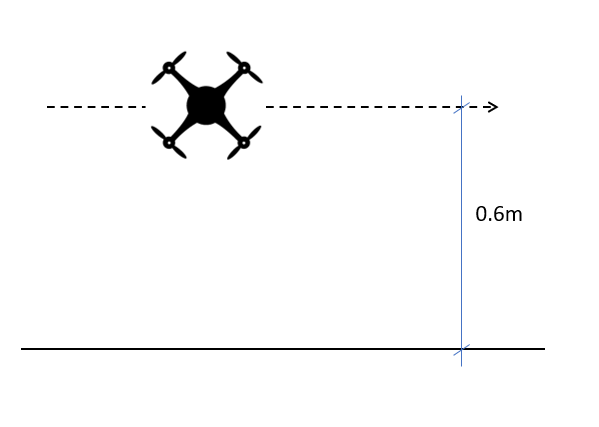
\includegraphics[width=0.28\textwidth]{modules/uneven_a}
    }
    \quad
    \subfloat[Stepped ground\label{fig:uneven_b}]{
        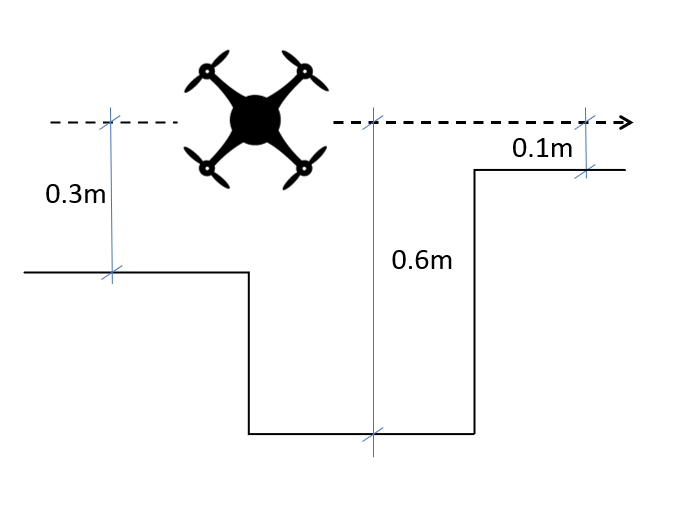
\includegraphics[width=0.28\textwidth]{modules/uneven_b}
    }
    \quad
    \subfloat[State estimator perspective of stepped ground\label{fig:uneven_c}]{
        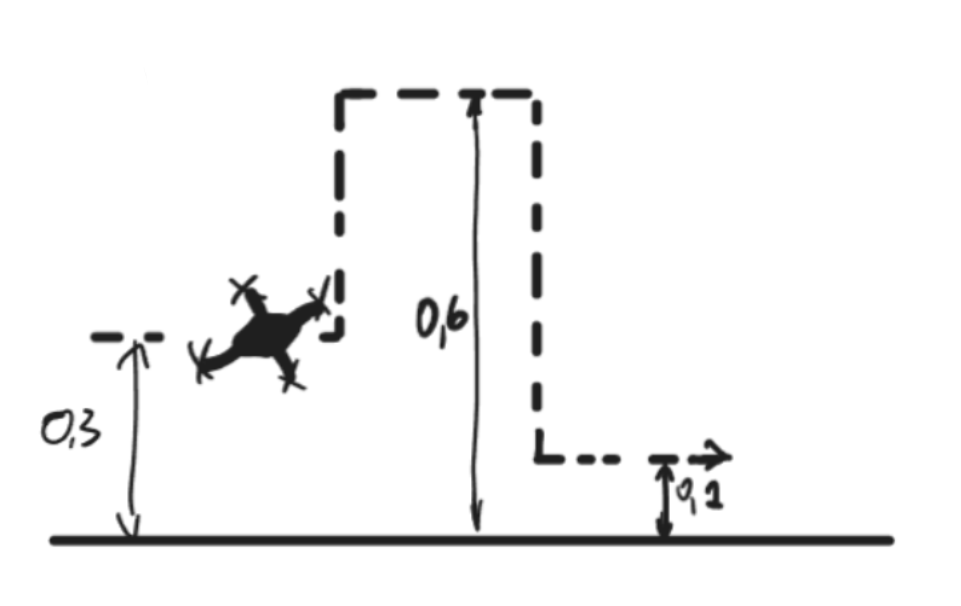
\includegraphics[width=0.28\textwidth]{modules/uneven_c}
    }
    \caption{Uneven floor problem.}\label{fig:uneven_floor}
\end{figure}

In the first Figure~\ref{fig:uneven_a}, the drone is flying over a flat ground, so the height sensor will contribute to the state estimate with the sensed value of 0.6 meters, which helps the State Estimator to provide a better estimate of the state (at least for the variable related with the height of the drone).

In the second Figure~\ref{fig:uneven_b}, the drone flies over a stepped ground. 
The height sensor will provide the State Estimator with a variable height by moving over this surface. 
The measured height will be either 0.6 or 0.1 meters, depending on the position.

Since the State Estimator is not aware of the conformation of the ground, the information perceived is the same as if the ground was flat and the drone was rapidly changing its height, as shown in Figure~\ref{fig:uneven_c}. 
The rapid change in the state estimate is not expected and can produce some instabilities in the flight.

To better understand the phenomena, we run some experiments with the following settings:
We placed a Crazyflie 2.1 with a height sensor attached in front of a cube-shaped obstacle with a height of 0.5 meters. 
We then write a script to take off the drone at 0.7 meters altitude and proceed above the obstacle. 
After passing the obstacle, the drone was supposed to land. 

As expected, as soon as the drone flies over the obstacle, the height sensor deck passes from a measure of 0.7 meters to a measure of 0.2 meters. 
This (unwanted) rapid change always makes the drone crash. 

To bypass this problem, we added a parameter that turns the height sensor's contribution to the state estimate on or off.
This way, when the application's environment has flat ground, the developer can enable the contribution and better estimate the drone's height.
Conversely, when the ground is uneven, the developer can avoid the problem described above by simply disabling the contribution through the parameter. 

\section{Lighthouse Module}\label{sec:module_lighthouse}

The Lighthouse ECF Module is the ECF Module associated with the Lighthouse Deck. As described in Section~\ref{subsec:absolute_positioning_systems}, the Lighthouse deck is a part of the absolute positioning system Lighthouse.
The Lighthouse positioning system consists of two (or more) base stations emitting infrared light signals in a sweeping pattern. 
The Lighthouse deck picks up these signals, which is mounted on the Crazyflie 2.1 drone. 
The deck then uses the received signals to calculate its precise position and orientation in 3D space.

This Module does not have a meaningful state. All the information that would belong to its state is technical and not applicable to any application.
Given this, the Lighthouse ECF module is an exception in the standard ECF Module implementation: it neither handles nor maintains a State.

A natural question can be: if the Lighthouse ECF Module does not hold a state, why is it useful?
To answer this question, we need a little bit of background on the functioning of the Lighthouse positioning system:
The Lighthouse positioning system is the most accurate and efficient positioning system that the whole Crazyflie platform provides. 
The problem related to this positioning system is the complex configuration.

The computation of the position in 3D space by knowing only the sweep angles of IR beams is not so direct. 
Indeed, to work correctly, the Lighthouse system needs a very accurate configuration based on multiple measurements taken in the flight space.

In fact, before using the Lighthouse, we need to estimate the environment's geometry. 
The system's geometry estimates the position and orientation of the two Lighthouse Base Stations with respect to the origin of the absolute positioning system.
To perform this estimation, the developer needs to measure the Geometry in multiple points of the flight space, and then by averaging them, he can get the best possible estimate.
The more accurate the Geometry estimation, the more precise the positioning system.

To answer the previous question, the Lighthouse ECF module exists and is extremely useful to overcome this limitation while using this positioning system.
The Lighthouse ECF Module is an ECF Module without state; it comprises numerous utility functions that help configure the Lighthouse positioning system.

The Lighthouse ECF Modules provide three main utility functions, each of which corresponds to a geometry estimation process:
\begin{itemize}
    \item \textit{simple\_geometry\_estimation}
    \item \textit{multi\_bs\_geometry\_estimation}
    \item \textit{automatic\_geometry\_estimation}
\end{itemize}
The first estimation process, \textit{simple\_geometry\_estimation}, is a very primitive and quick approach to the Geometry estimation process. 
It consists of a single measurement in one position in the 3D space. 
When this utility function is called, the ECF Module asks Crazyflie 2.1 for a single estimation of the position and orientation of the Lighthouse Base Stations.
When this information is received, the Module sets the measurement point as the origin of the 3D coordinate system. 
After that, it uploads this configuration back to Crazyflie 2.1.

A problem related to this type of estimation is that the error in the estimate is non-constant in the flight space. 
This problem happens because we only have a single measure in the entire flight space. 
As evident from Figure~\ref{fig:lighthouse_error_1}, it increases proportionally to the distance from the origin.
In this case, the resulting position estimate in the 3D space around the origin would be accurate. 
Still, as far as we move from the origin, the error in the drone position estimate will increase, possibly resulting in instabilities or even crashes.
This estimation process is intended only for quick tests where the drone position does not deviate too much from the origin.

\begin{figure}[tb]
    \centering
    \subfloat[Error distribution in the flight space while using the \textit{simple\_geometry\_estimation}\label{fig:lighthouse_error_1}]{
        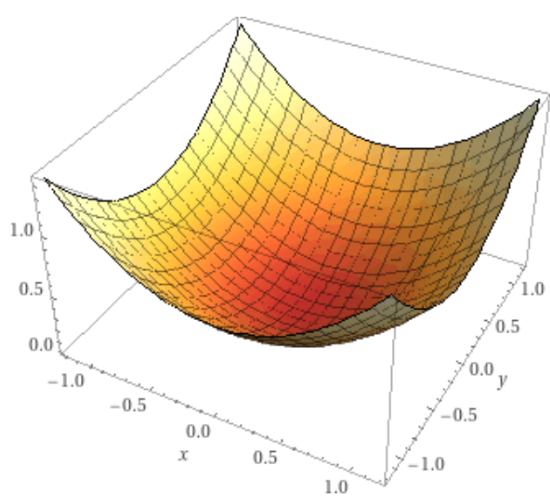
\includegraphics[width=0.40\textwidth]{modules/lighthouse_error_1}
    }
    \qquad
    \subfloat[ Error distribution in the flight space while using the \textit{multi\_bs\_geometry\_estimation}\label{fig:lighthouse_error_2}]{
        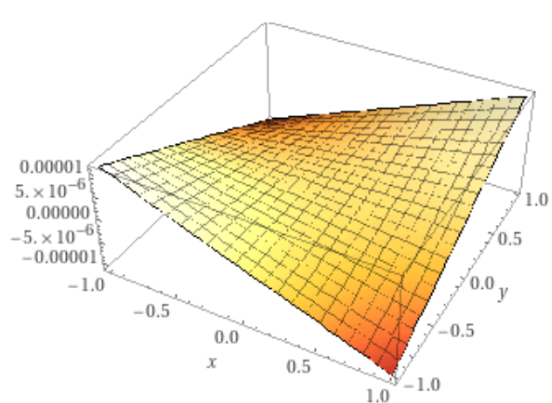
\includegraphics[width=0.40\textwidth]{modules/lighthouse_error_2}
    }
    \caption{Error distribution for Lighthouse.}\label{fig:lighthouse_error}
\end{figure}

To overcome this significant limitation, we developed a more accurate estimation process: \textit{multi\_bs\_geometry\_estimation}. 
As shown in Figure~\ref{fig:lighthouse_error_2}, this estimation process tries to make the error in the estimate constant across the entire flight space. 
Moreover, this estimation method also supports the presence of multiple Lighthouse Base Stations (more than 2) that significantly increase flight space.

This estimation method consists of multiple executions of the first estimation process.
All the recorded samples are averaged to build the most accurate geometry estimation sent to the Crazyflie 2.1.


The only drawback of this last estimation process is that it requires human help while doing the process. 
The problem is that the user moving the drone around the drone in the fourth phase is interfering with the estimation process. 
The user's body can block the IR beams from some base stations, invalidating lots of samples that otherwise would have been useful to compute a better geometry estimation.

The last estimation process, the \textit{automatic\_geometry\_estimation}, is the automation of the previous process. 
The user can configure the execution as he wants, and then the ECF Module (with the help of the Flow Deck v2) performs the sampling process by autonomously moving the drone around the flight space.

The \textit{automatic\_geometry\_estimation} is the most complex but most powerful estimation process.

\section{AI deck Module}\label{sec:module_ai_deck}


The AI Deck is an accessory board designed to provide on-board artificial intelligence (AI) capabilities to the Crazyflie 2.1, allowing it to perform advanced computational tasks without needing external processing.

The AI Deck is equipped with a powerful microcontroller unit (MCU) and a field-programmable gate array (FPGA), enabling high-performance computing and direct machine learning inference on the drone.
The MCU on the AI Deck can run complex algorithms and execute machine learning models. 
The FPGA complements the MCU by accelerating certain computations and enhancing the overall processing capabilities.

The AI Deck can communicate directly with the ground station via WiFi thanks to the NINA unit mounted on the deck.
The AI Deck, by default, runs a program on its MCU, which makes the video streaming of the camera mounted with the deck available on the WiFi communication channel.
For this work, we adopted this standard configuration of the AI Deck without implementing any algorithm for object tracking or anything similar.

The AI Deck ECF Module is an ECF module that allows one to connect, view, and run algorithms on the video streamed by the AI Deck itself.
When this ECF module is detected and created, it automatically tries to connect to the WiFi acces point held by the deck.

In particular, the Module consists of the following utility functions:
\begin{itemize}
    \item \textit{record}
    \item \textit{show\_recording}
    \item \textit{run\_ai}
\end{itemize}

The utility function \textit{record} allows the user to record from the video stream a video in mp4 format. 
This functionality is significant when the user is in the developing phase of an AI algorithm. 
In this case, the user can record videos and test/train their models using a flight recording.

The \textit{show\_recording} utility simply pops up a video player with the last unsaved recording, or if the path to the filename is provided, it shows the recording located at that path.

When the developer has completed its AI algorithm, the user can use the \textit{run\_ai} utility to run that algorithm on the real-time streaming from the camera and perform the actions needed to accomplish the goal of the application to be developed.

The \textit{run\_ai} function takes in input the algorithm (a python function) and an arbitrary list of arguments that can be used to take the actions.

This function looks very similar to a Subscription in our Coordination Manager with an Action (the algorithm) and a Context (the arguments) to an Observable that maintains the video stream.

Even if we could use our Coordination Framework, we decided to keep this particular implementation outside of it on purpose for two main reasons:
First, we did not want to overload the Coordination Framework with heavy data like images to make the complete state lighter.
Secondly, we thought that a direct implementation of the \textit{run\_ai} function would have been much easier to use in this case with respect to the standard subscription mechanism across the Coordination Framework.


\chapter{Conclusions and future developments}
\label{ch:conclusions}
The evaluation of a drone programming system is crucial to assess its effectiveness, performance, and suitability for specific applications. 
This chapter aims to provide a comprehensive evaluation of EasyFly. 
The baseline used to compare our programming environment is the basic Crazyflie python library (cflib) 

We divided the evaluation process into two main topics: qualitative and performance analysis.

In the first step, we will give a qualitative analysis of EasyFly and an understanding of the strengths and leaks of our programming system.
For this analysis, we participated in the challenges organized for the Digital Futures Drone Arena project~\cite{dronearena}.
During this challenge, groups of students and enthusiasts were asked to complete an obstacle run using Crazyflie 2.1 nano drones.

Then, we will move to performance analysis of EasyFly in a real example implementation, comparing it with a similar implementation written using only the core cflib.
This evaluation aims to assess the ease of implementing a drone application with EasyFly and the consequent reduction in complexity in the scripts. 
On the other hand, we will demonstrate that the performance of an application developed with EasyFly is almost the same as the implementation using the core cflib offered by Crazyflie.

Given the high complexity of performance evaluation of drone applications, we designed and implemented a simulation environment for EasyFly.
This simulation environment allowed us to conduct a precise performance analysis without deviating from the real environment's performance.

\section{Qualitative Analysis}\label{sec:qualitative_analysis}
In the HDI domain, the research's core part, especially from the computer science perspective,
is the experimental phase. During this phase, researchers put their ideas and prototypes to test
and assess the practicality of innovative interaction models.

For a programming environment like EasyFly, testing and evaluating in a real research scenario in HDI is essential. 
The testing in real scenarios can help detect possible weaknesses in the programming environment, allowing for fine-tuning the model.

To best evaluate our EasyFly programming environment, we had the possibility to participate in the Digital Futures Drone Arena project~\cite{dronearena}.

The Drone Arena project planned two challenges where groups of students and enthusiasts with different backgrounds were asked to complete a specific task using drones.
These challenges aim to allow researchers to collect data and perform studies about human-drone interactions.

The EasyFly programming environment was part of the inaugural challenge in Sweden in June 2022~\cite{dronearenaChallenge}. 
In this challenge, five groups of students and enthusiasts with knowledge of computer science were asked to program Crazyflie 2.1 nano drones to complete an obstacle course.
There were two main alternatives to write the scripts: the standard cflib or the EasyFly programming environment. 

The challenge was distributed over three days; the first two days were dedicated to development and testing, and the last day was dedicated to the final challenge.%, where the groups competed with each other with what they had produced in the days before.

On the first day, we gave the groups a brief presentation on the basic knowledge of the Crazyflie 2.1 platform. 
We also described the main components and working principles of the EasyFly programming environment.

Then, we provided the groups with a Python project, where inside was the original cflib, our EasyFly programming environment, and a folder of examples for both.
From then on, the groups were free to develop and test the code with real Crazyflie 2.1 in a sample stage, with minimum support from the research team.

This particular setting of the challenge allowed us to see and measure the impact of using EasyFly on a group with minimum knowledge of the Crazyflie platform. 
On the final day of the challenge, 2 out of 5 teams decided to participate in the final using our EasyFly programming environment. 

The approach for all the groups was to use a Multiranger deck and perform a hand-driven flight through the obstacle course.
The main differences were how the groups implemented the mechanism that allowed them to push or pull the drone using their hands.

By analyzing the code that all the groups produced, we noticed two main aspects of the usage of the EasyFly programming environment:
The groups that started using EasyFly from the beginning developed more complex solutions.
The code of the groups that used the programming environment looked clean and simple, even if the solution they implemented was more complex.

Although we expected more adhesion on EasyFly, we noticed that almost all the groups had a look at the code of the programming environment, in particular inside the utility functions of the ECF modules. 
In their final code, almost every group used the utility functions of the Multiranger ECF Module, either directly or indirectly.

In conclusion, the challenge of the Drone Arena project allowed us to understand that the entire EasyFly programming environment, particularly the Coordination Manager, can seem too complicated at first glance and was a little more complex than we thought.
The groups that decided not to use the programming environment decided on purpose to develop a more simple and sometimes effective solution.


\section{Performance Analysis}\label{sec:performance_analysis}

EasyFly is a programming environment that aims to ease the development of drone applications, reaching the same solution with less effort, both in terms of time to write the solution and expertise required to implement the solution.
Even if simplicity remains the first objective, performance plays an important role in the EasyFly programming environment.
If the programming environment is easy to use but, in the end, results in inefficiency in terms of performance, it automatically becomes useless.

To assess the performance of EasyFly, we compared it with the standard implementation of Crazyflie's cflib across two real example applications used in HDI research.
The first application scenario takes place in an artistic exhibition between a human performer and a drone. 
The second application scenario is an obstacle course similar to the Drone Arena inaugural challenge~\cite{dronearenaChallenge}.

In this analysis, we will demonstrate that the expected loss in performance with respect to the basic cflib implementation is shallow compared to the reduction of program complexity.

\subsection{EasyFly Simulation Environment}\label{subsec:simulation_environment}
Measuring performance in drone applications is a very hard task, and usually, the performance of the applications can vary highly across different runs.
When running the application in a real environment, the performance of the applications can usually vary highly across different runs.
Given the fact that the conditions of the environment influence performance, the only possible strategy to measure performance is to execute and sample the same scenario multiple times and then average the results.
Of course, this approach can have a high cost in terms of time and resources consumed.

To simplify the evaluation process and collect more precise data, we developed a simulation environment for EasyFly.
In the simulation environment, the drones are replaced by a virtual copy that replicates the drone's movements in a controlled simulation.
The simulation allows the reduction of the influence of the environment on performance measurements to zero, enabling precise performance measurement with a single run.
This approach drastically reduces the costs of the analysis.
A possible drawback of a poorly accurate simulation environment is that the performance can deviate from the real application performance.

In our simulation environment, we create a virtual Crazyflie 2.1 that emulates a real Crazyflie 2.1.
Upon receiving the commands from the ground station, the virtual Crazyflie computes and updates its internal state (position, velocity, acceleration, and some sensor measures) and sends back data.
In the current implementation of the EasyFly simulation environment, the virtual Craziflie emulates the control-related commands, logging, and parameter features.

As shown in Figure~\ref{fig:simulation_environment}, the virtual Crazyflie communicates with the ground station's script using a UDP channel.
Usually, the ground station script and the simulated Crazyflie run on the same machine, so the UDP communication is local.

The script of the ground station is entirely independent of Crazyflie's software. 
The execution and performance of the ground station's script are not affected by whether the Craziflie is virtual or not.
This separation guarantees that the performance measured with EasyFly's simulation environment does not deviate from the real environment.

\sidecaptionvpos{figure}{b}
\begin{SCfigure}[\sidecaptionrelwidth][h]
    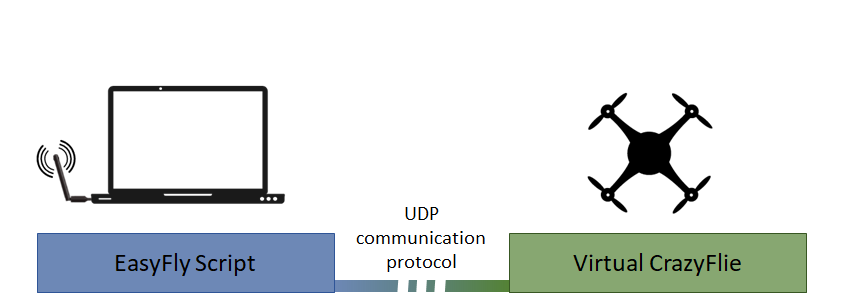
\includegraphics[width=0.5\textwidth]{evaluation/simulation_environment}
    \caption{Structure of EasyFly simulation environment.}\label{fig:simulation_environment}
\end{SCfigure}


\subsection{Application Scenario Evaluated}\label{subsec:application_scenario_evaluated}
To best evaluate the performance of any system, it is crucial to select the appropriate application scenario.
In particular, it is essential to test the system in a scenario that is as close as possible to an actual application of this system.

Given that our programming environment is designed to build drone applications for HDI research, we selected two representative application scenarios from the literature on HDI.

The first application takes inspiration from recent research conducted in the field of HDI~\cite{eriksson2020ethicsInMovement}. 
This research explored how ethicality is shaped in the interaction between a choreographer, a performer, and a choir of five drones performing together on the opera stage.
In our simplified version of this scenario, we reduced the drones to a single drone. 
Moreover, the choreography designed for the drone is determined before the performance.
In other words, our drone should follow a predetermined path on the stage, exhibiting with the performer. 
The drone should also implement an obstacle avoidance mechanism to avoid any collision on the stage.
In Figure~\ref{fig:exhibition}, we can see the trajectory followed by the virtual Crazyflie during the performance measurement of this application.

The second application we selected for performance analysis is an obstacle course similar to the one adopted for the inaugural challenge of the Digital Futures Drone Arena project~\cite{dronearenaChallenge}.
In this application, we based the implementation of the algorithm on an elevation model of the environment. 
In other words, we modeled the obstacle course stage with a grid where every cell contains the elevation at that coordinate.
We then implemented a script to navigate safely in the provided environment. 
We also adopted the obstacle avoidance mechanism in this application to avoid unpredicted crashes.
In Figure~\ref{fig:obstacle_course}, we can see the trajectory followed by the virtual Crazyflie during the performance measurement of this application.

\begin{figure}[t]
    \centering
    \subfloat[First application scenario: drone exhibition\label{fig:exhibition}]{
        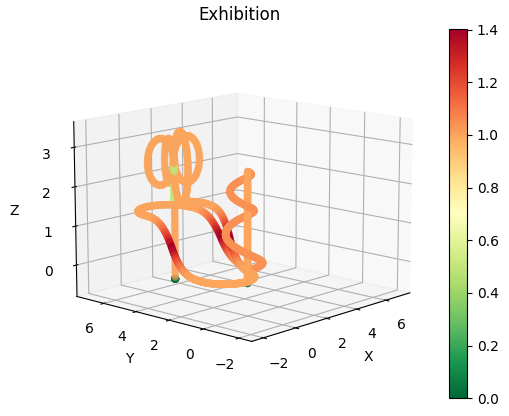
\includegraphics[width=0.45\textwidth]{evaluation/exhibition}
    }
    \quad
    \subfloat[Second application scenario: drone obstacle course\label{fig:obstacle_course}]{
        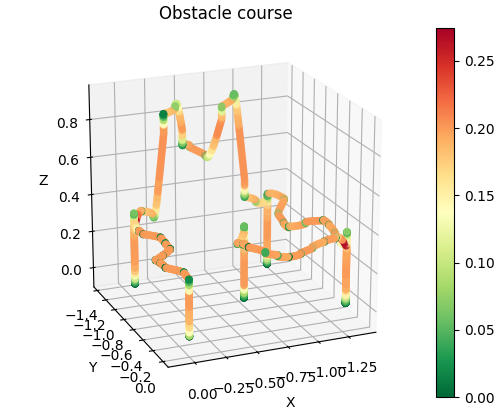
\includegraphics[width=0.45\textwidth]{evaluation/obstacle_course}
    }
    \caption{Application scenarios' trajectories.}\label{fig:application_traj}
\end{figure}

\subsection{Tools and Metrics for Measuring Performances}\label{subsec:performance_metrics}
As previously anticipated, our core objective is to produce a simple programming environment; given this, the most critical analysis is around the complexity of the applications.
Another important aspect to keep under control is the execution performance 

To evaluate our programming environment, we indeed targeted two main categories of performance metrics: complexity and execution performance.

The first category, complexity, is composed of a set of metrics that tries to evaluate the complexity of a program.
The category is composed of the following metrics:
\begin{itemize}
    \item Lines of Codes (LOC)
    \item Cyclomatic Complexity (CC)
    \item Halstead Metrics (HAL)
\end{itemize}

The LOC metric is the most simple measure of the complexity of a program. As the name suggests, it is the count of lines of code of the program under analysis.

The Cyclomatic Complexity is a Complexity analysis method proposed by Mccabe in 1996; it evaluates the complexity by measuring the number of linearly independent paths
through a piece of code~\cite{mccabe1996cyclomatic}.

The Halstead Metrics was introduced by Maurice H. Halstead in the 1970s. 
They are based on the analysis of the number of unique operators and operands in a program, as well as their occurrences~\cite{hariprasad2017software}.
The five main metrics proposed by Halstead are:
\begin{itemize}
    \item \textbf{Program Vocabulary} (\( \eta \)): The total number of unique operators and unique operands in the program. 
    It is given by the formula: \( \eta = \eta_1 + \eta_2 \) where \( \eta_1 \) is the number of distinct operators, and  \( \eta_2 \) is the number of distinct operands.
    \item \textbf{Program Length} (\( N \)): The total number of operator occurrences and operand occurrences in the program. It is given by the formula: \( N = N_1 + N_2 \), where \( N_1 \) is the total number of operators and \( N_2 \) is the total number of operands.
    \item \textbf{Program Volume} (\( V \)): A measure of the size of the program. It is given by the formula: \( V = N \log_2 \eta \).
    \item \textbf{Program Difficulty} (\( D \)): Represents the complexity of the program. It is given by the formula: \( D = \frac{\eta_1}{2} \cdot \frac{N_2}{\eta_2} \).
    \item \textbf{Effort} (\( E \)): Represents the effort required to understand and develop the program. It is given by the formula: \( E = D \cdot V \).
\end{itemize}

To collect all these measurements, we used \textit{radon}~\cite{radon}, a Python library that computes all such metrics using static analysis on the source code of the scripts.

The second category of metrics, the execution performances, is a set of metrics that measures the resource consumption of the scripts.
The category is composed of the following metrics:
\begin{itemize}
    \item Memory (RAM) consumption
    \item Average CPU consumption 
    \item Max CPU consumption
    \item Network load
\end{itemize}

These metrics provide valuable insights into the efficiency and resource utilization of the scripts. 
Memory consumption indicates how much random access memory is being used. 
Average CPU consumption gives an idea of the overall CPU usage over a period, max CPU consumption highlights the peak CPU usage, and network load measures the amount of data transmitted over the network during script execution.

Analyzing these metrics is crucial for identifying potential bottlenecks and ensuring resource utilization does not constrain our programming environment.

The machine used to run the performance analysis mounts an AMD Ryzen 7 5700U with Radeon Graphics with 8GB of RAM.
To measure the memory consumption, we used \textit{memory-profiler}~\cite{memoryProfiler}, a Python library for collecting RAM usage while executing a Python script.
We used the \textit{Performance Monitor} tool for Windows for the CPU metrics. 
Finally, the simulation environment automatically computes the network load by summing all the CRTP received and sent.

\subsection{Results Analysis}\label{subsec:result_analysis}
This section will present the complexity and performance analysis results aimed at evaluating our EasyFly programming environment.

As described in Section~\ref{subsec:application_scenario_evaluated}, we selected two application scenarios that best represent our target application.
Since our primary goal is to produce a simple programming environment that researchers of HDI can use, this evaluation tries to asses the simplicity of the environment while not losing too much in performance. 

As we have seen in Section~\ref{subsec:performance_metrics}, we divided the evaluation into two categories:
\begin{itemize}
    \item Complexity analysis
    \item Performance analysis
\end{itemize}

The complexity analysis represents the core part of the evaluation and is composed of three metrics:
\begin{itemize}
    \item Lines of Codes (LOC)
    \item Cyclomatic Complexity (CC)
    \item Halstead Metrics (HAL)
\end{itemize}

\begin{figure}[t]
    \centering
    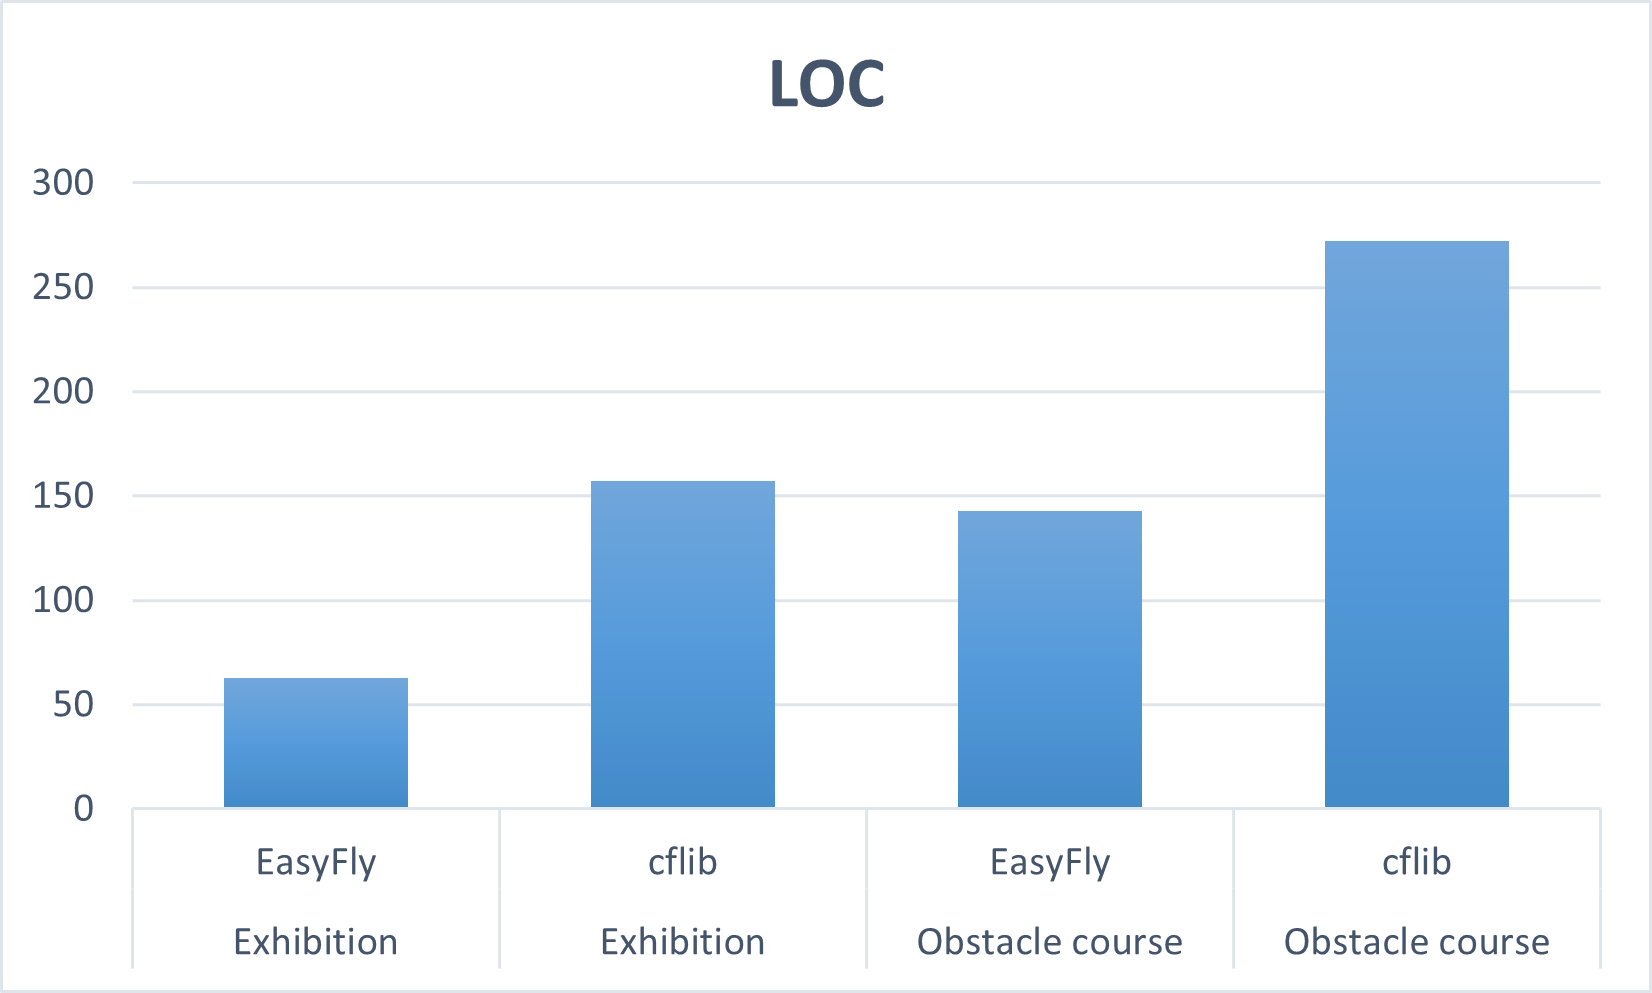
\includegraphics[width=0.6\textwidth]{evaluation/loc}
    \caption{Lines of Code.}\label{fig:loc_count}
\end{figure}

Looking at the results, it is crystal clear that our programming environment, EasyFly, is much less complex than the original cflib we selected as a baseline for comparison.
Starting from the most straightforward metric, LOC, we can see in Figure~\ref{fig:loc_count} that the results are, in both scenarios, halving the count.
EasyFly, with respect to cflib, allows you to write the same application with half of the code.

\begin{figure}[t]
    \centering
    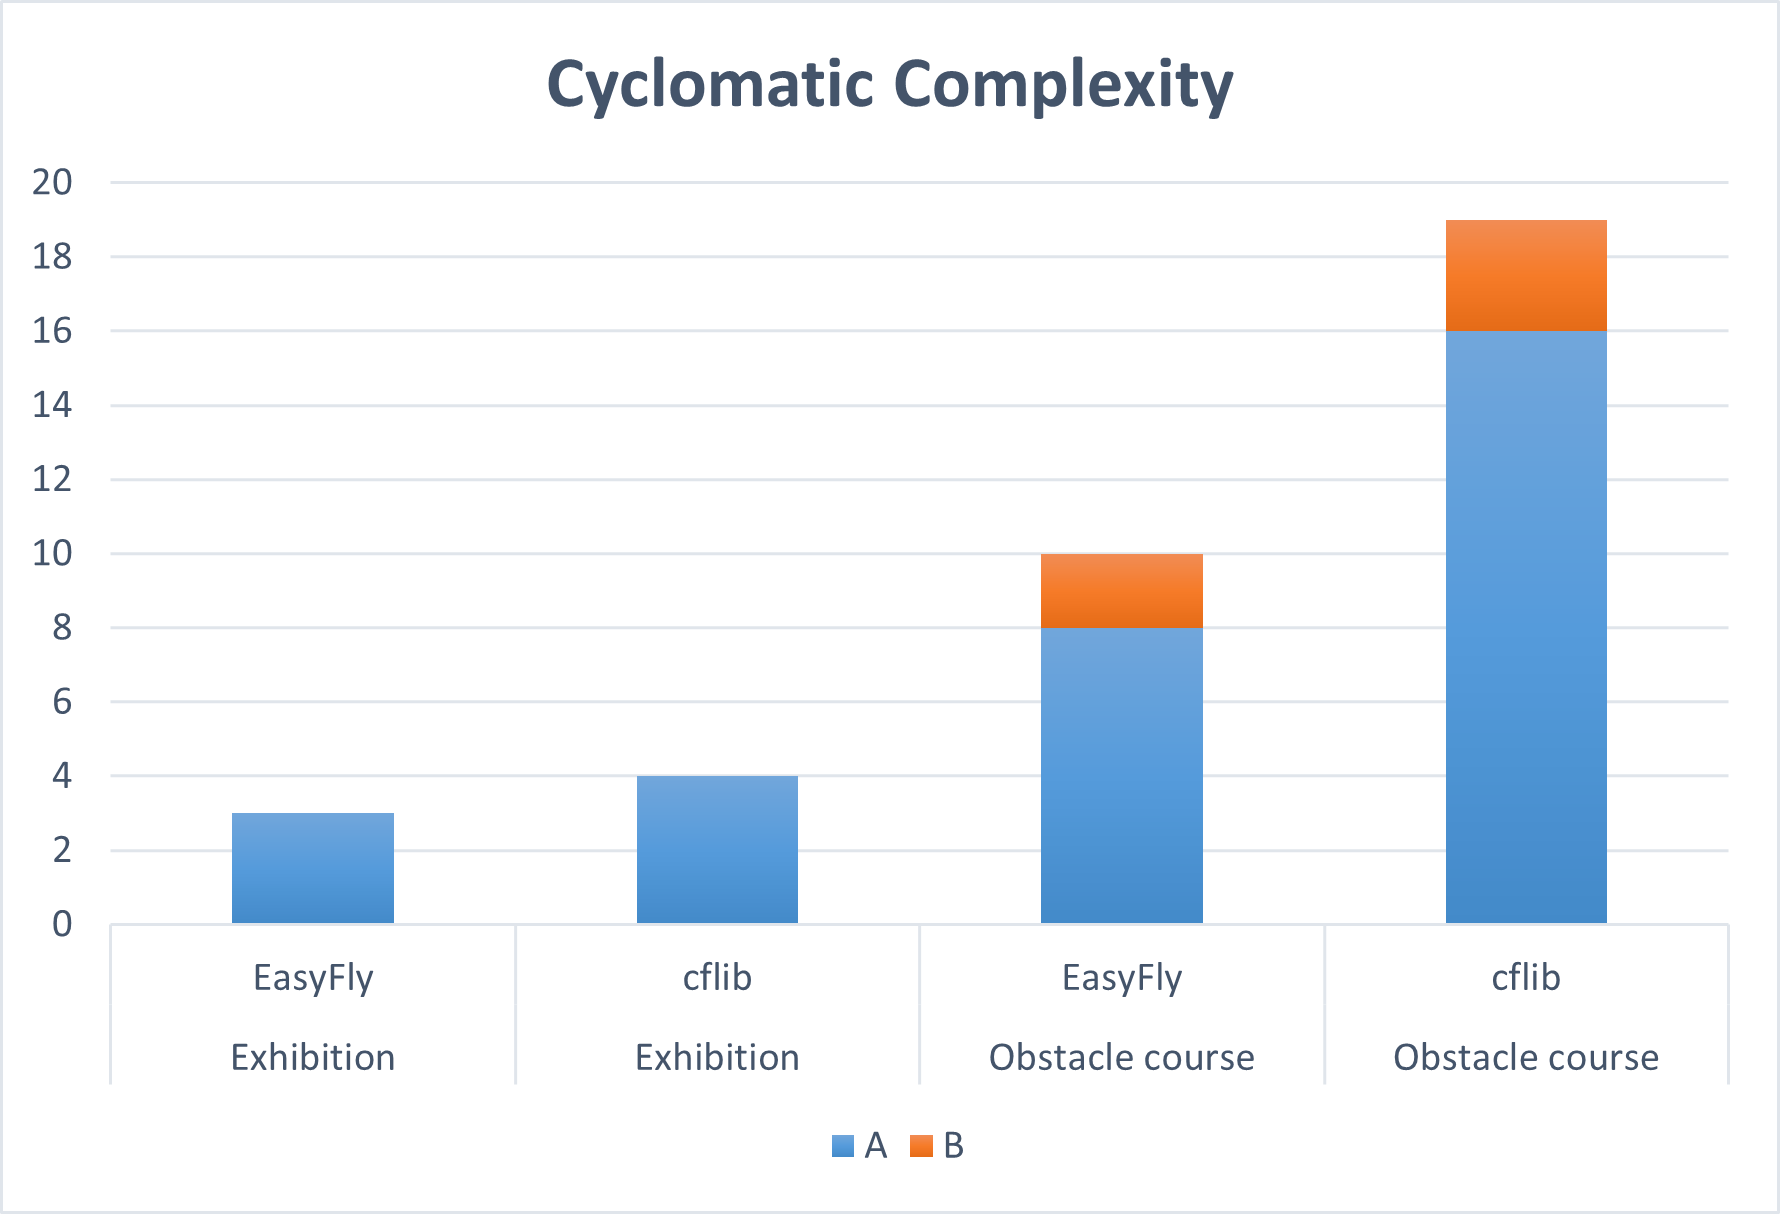
\includegraphics[width=0.6\textwidth]{evaluation/cc}
    \caption{Cyclomatic Complexity.}\label{fig:cc}
\end{figure}

By looking at the second metric, CC, we can see, also in this case, the same trend.
Moreover, when comparing the CC across the two different scenarios, it is evident that the performance gap between cflib and EasyFly increases with complexity.
In Fact, in the second scenario, the obstacle course, the total CC computed is 50\% less than the cflib's implementation.

The last metric for complexity, HAL, by looking at the results in Table~\ref{table:HAL}, confirms what we previously said for LOC and CC. 
In particular, in this case, it is much more evident that the performance gap between cflib and EasyFly increases with complexity.
Here, for the Effort (\( E \)), we observed a gap of over 55\% for the second scenario.

\begin{table}[b]
    \centering
        \begin{tabular}{*{6}{|c}|}
        \hline
        \rowcolor{bluepoli!40}
        \textbf{Scenario} & \textbf{\( \eta \)} & \textbf{\( N \)} & \textbf{\( V \)} & \textbf{\( D \)} & \textbf{\( E \)}\\
        \hline \hline
        Exhibition with cflib & 33 & 45 & 226.99 & 4.04 & 916.72 \\
        \hline
        Exhibition with EasyFly & 38 & 48 & 251 & 3.0 & 755.70 \\
        \hline \hline
        Obstacle course with cflib & 171 & 296 & 2195.68 & 8.74 & 19187.76 \\
        \hline
        Obstacle course EasyFly & 108 & 168 & 1134.82 & 7.66 & 8696.31 \\
        \hline
        \end{tabular}
        \\[10pt]
        \caption{Halstead Metrics.}\label{table:HAL}
\end{table}

In the second part of the evaluation, the performance analysis, we expect a slight loss in performance due to the overhead introduced by the EasyFly main components.
In fact, by looking at Table~\ref{table:cpu_consumption}, we can see that the CPU percentage utilization is generally less when using the standard cflib with respect to EasyFly.

The reason for this increase in CPU utilization is that EasyFly handles most things automatically. 
An important observation needs to be around the average CPU consumption. 
In this measurement, we can see that the metrics for EasyFly are not so far from the standard cflib, and, in the first more straightforward scenario, it is also better.
These metrics indicate that EsayFly is more flexible and better adapts resource utilization across different situations.

\begin{table}[t]
    \centering
        \begin{tabular}{*{3}{|c}|}
        \hline
        \rowcolor{bluepoli!40}
        \textbf{Scenario} & \textbf{CPU Average (\%)} & \textbf{CPU MAX (\%)} \\
        \hline \hline
        Exhibition with cflib & 0.570 & 12.829 \\
        \hline
        Exhibition with EasyFly & 0.266 & 16.449 \\
        \hline \hline
        Obstacle course with cflib & 0.540 & 18.423 \\
        \hline
        Obstacle course EasyFly & 0.625  & 22.340 \\
        \hline
        \end{tabular}
        \\[10pt]
        \caption{CPU consumption.}\label{table:cpu_consumption}
\end{table}

The memory consumption metric is a weakness for EasyFly. 
In particular, it is clear from the results shown in Figure~\ref{fig:ram_usage} that the standard cflib is consuming less than 50\% of EasyFly for the same application scenario.
Also in this case, the overhead is due to all the infrastructure needed to manage most of the tasks automatically.
Even if the memory consumption metric is a weakness for EasyFly, we can anyway learn two important facts:
The first is that memory consumption is in the order of hundreds of MiB; hence, any modern machine can handle such memory load with any problem.
The second fact is that by increasing the complexity of the application scenario, the gap between the cflib and EasyFly is constant; 
this suggests that the memory consumption will never drift from the performance of the standard cflib.

\begin{figure}[t]
    \centering
    \subfloat[Scenario: exhibition with cflib\label{fig:mem_ex_cflib}]{
        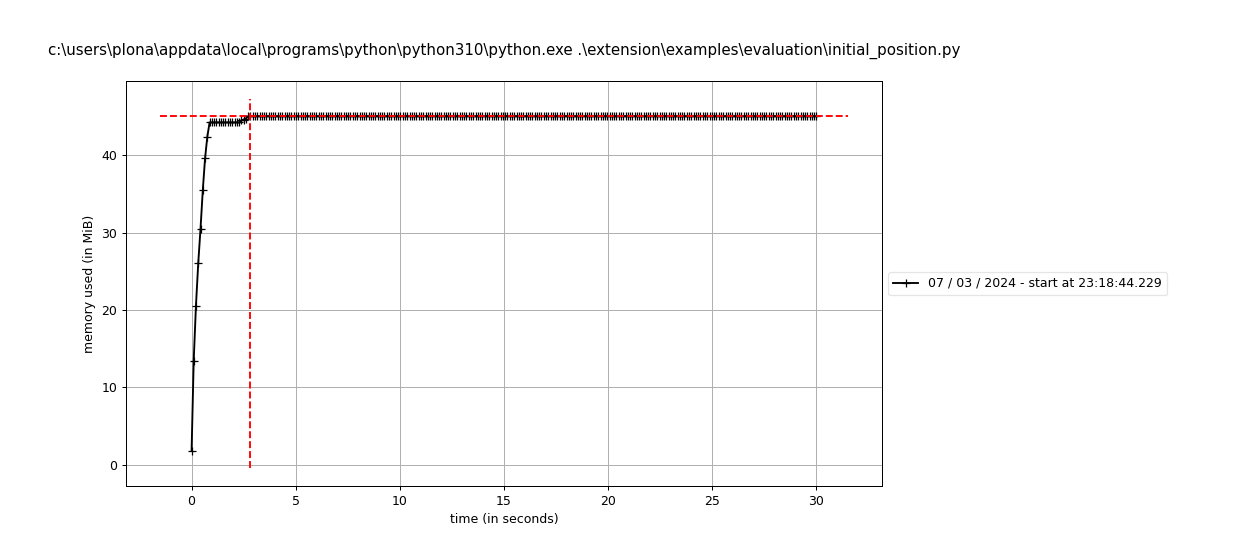
\includegraphics[width=0.45\textwidth]{evaluation/exhibition_cflib_mem}
    }
    \quad
    \subfloat[Scenario: exhibition with EasyFly\label{fig:mem_ex_ecf}]{
        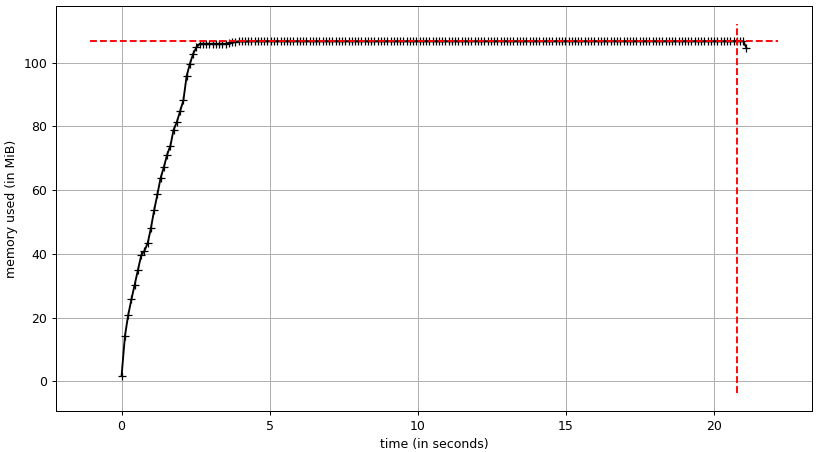
\includegraphics[width=0.45\textwidth]{evaluation/exhibition_ecf_mem}
    }
    \quad
    \subfloat[Scenario: obstacle course with cflib\label{fig:mem_obs_cflib}]{
        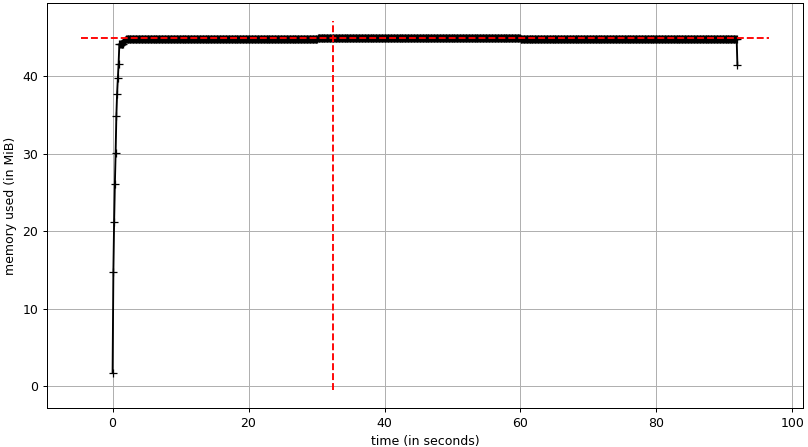
\includegraphics[width=0.45\textwidth]{evaluation/obstacle_course_cflib_mem}
    }
    \quad
    \subfloat[Scenario: obstacle course with EasyFly\label{fig:mem_obs_ecf}]{
        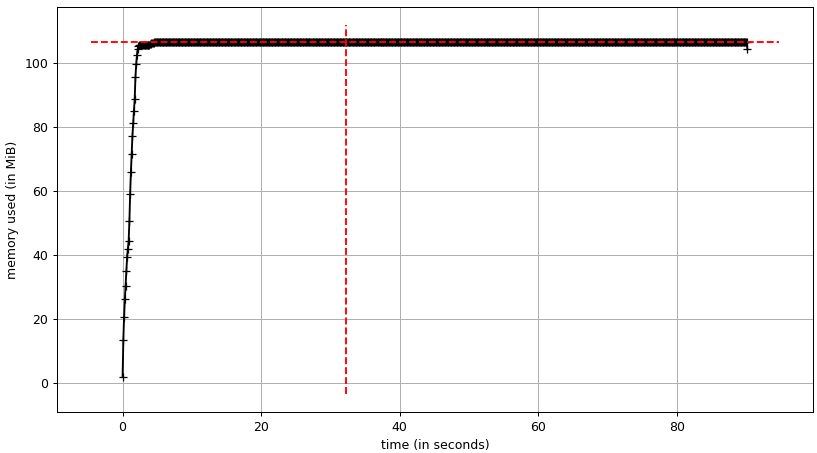
\includegraphics[width=0.45\textwidth]{evaluation/obstacle_course_ecf_mem}
    }
    \caption{Memory (RAM) usage.}\label{fig:ram_usage}
\end{figure}


The last metric for the performance evaluation is the network load. As previously described, the simulation environment helped greatly in retrieving such metrics. 
In particular, the simulation execution automatically computes the incoming and outgoing network load. 
In Figure~\ref{fig:network_load}, we can see the result of this computation, where we pointed out the outgoing and the incoming traffic load in KB for every application scenario.
The point of view of the measurement is that of the ground station. Out-packages have the direction from the ground to the drone, and In-packages follow the other direction. 
Thanks to the optimization made by the Communication Framework hosted on EasyFly, we can observe a slightly better result for the network load metric.
In particular, Easyfly automatically optimizes the logging task, reducing the cost of communication.

\begin{figure}[t]
    \centering
    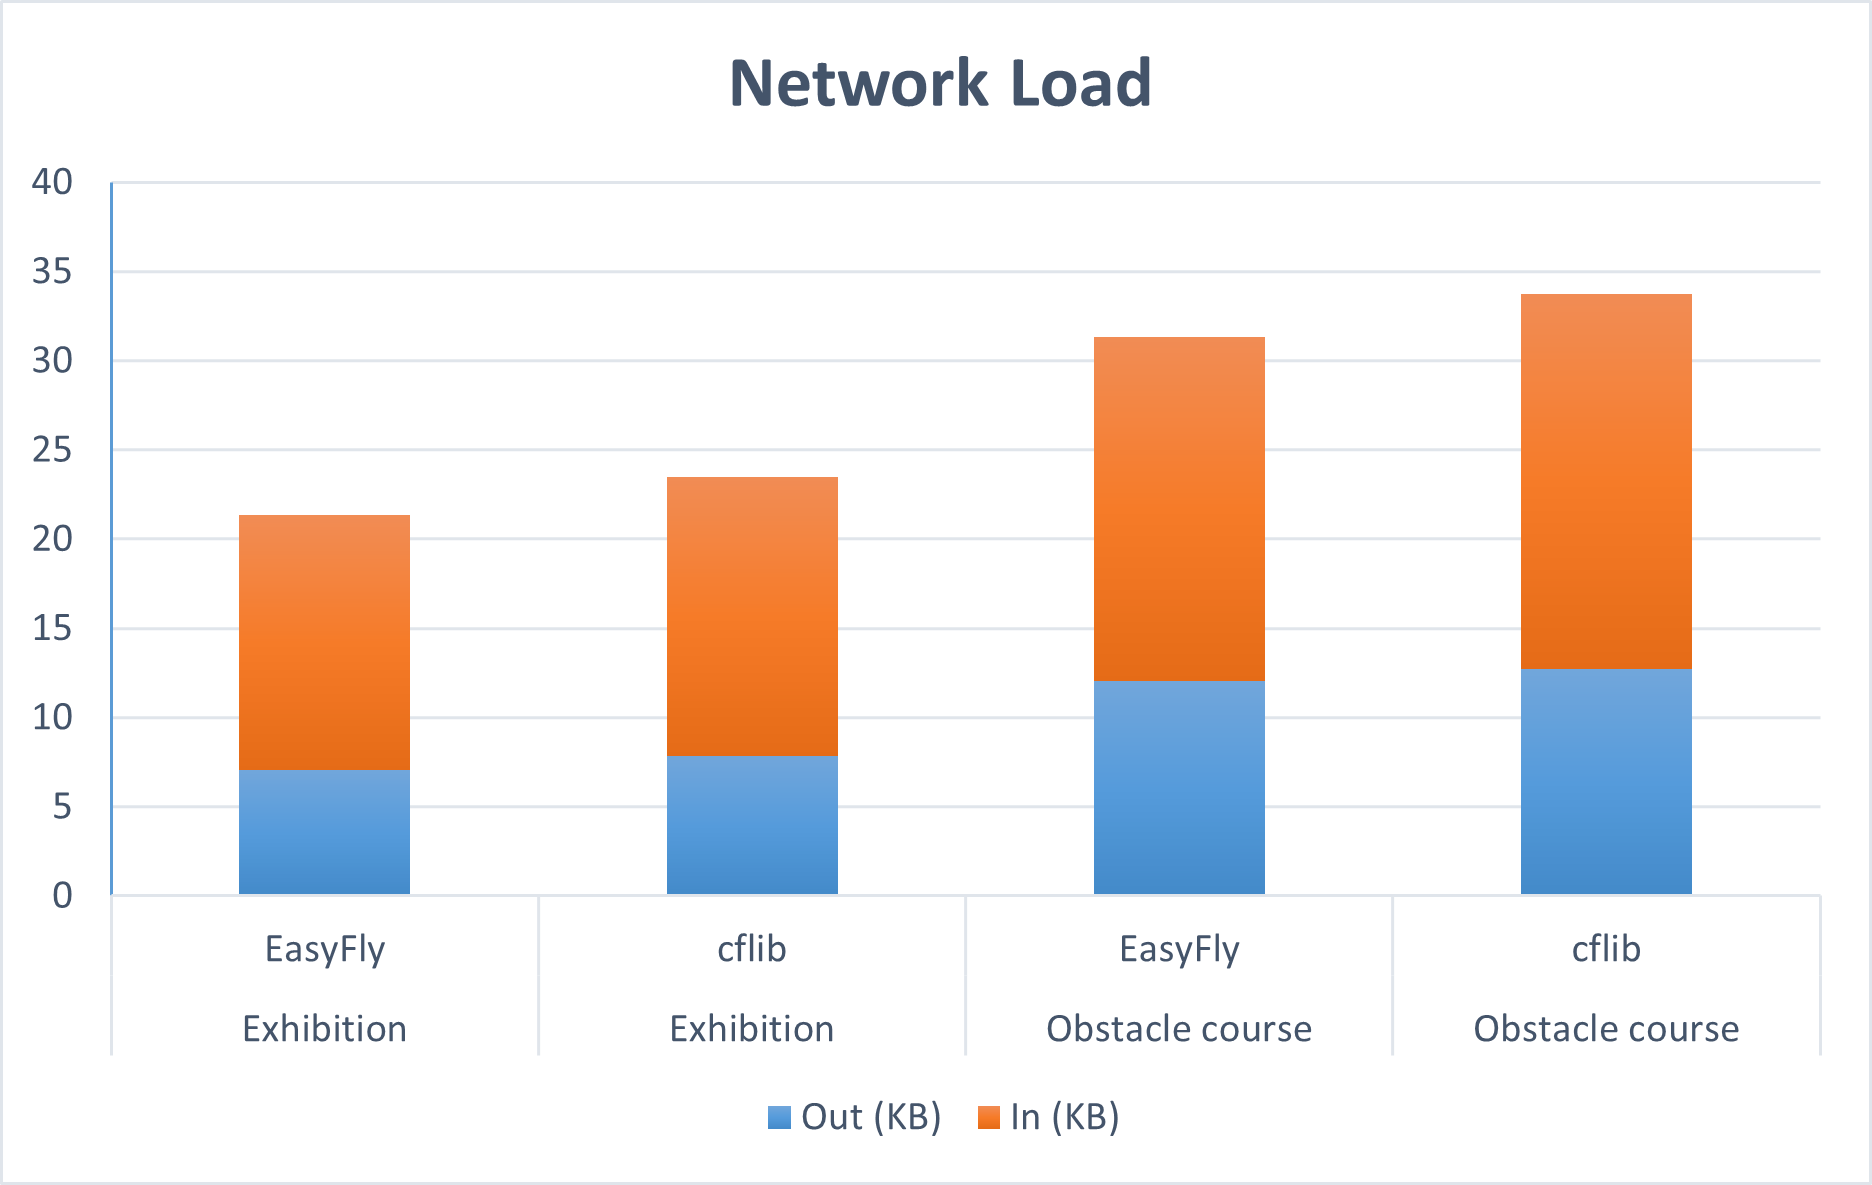
\includegraphics[width=0.6\textwidth]{evaluation/network}
    \caption{Network load.}\label{fig:network_load}
\end{figure}

In conclusion, as expected, we have observed that our programming environment, EasyFly, is significantly reducing the complexity of its scripts; 
On the other hand, the performance metrics are kept on the same level with respect to the standard cflib.

\subsection{Future Developement}\label{subsec:future_developement}
This thesis work mainly focused on drone application with a single drone deployment. 
This limitation clearly does not fit modern HDI research's needs. 

For this reason, a possible future development around the EasyFly programming environment is the possibility of deploying multiple drones without introducing useless complexity in the development phase.
In the actual implementation of the standard cflib there is a possibility of running scripts for swarm of drones.

EasyFly should extend this basic feature by integrating it within its Coordination Manager, allowing for inter-drone communication.

Another key point of future development should be around the simulation environment. 
For the purpose of this work, we used the simulation environment mainly to evaluate performance.
In our opinion, allowing the user to leverage the potentiality of such a system should be critical.

Testing with drones is costly; hence, having the possibility to rely on a solid simulation environment is essential.
A future version of our simulation environment should include the possibility of utilizing all the available sensors inside the simulation. 
Moreover, multiple drone deployments should be allowed inside the simulation to support swarm programming.

%-------------------------------------------------------------------------
%	BIBLIOGRAPHY
%-------------------------------------------------------------------------

\addtocontents{toc}{\vspace{2em}} % Add a gap in the Contents, for aesthetics
\bibliography{Thesis_bibliography} % The references information are stored in the file named "Thesis_bibliography.bib"

%-------------------------------------------------------------------------
%	APPENDICES
%-------------------------------------------------------------------------

\cleardoublepage
\addtocontents{toc}{\vspace{2em}} % Add a gap in the Contents, for aesthetics
%\appendix
%\chapter{Appendix A}
%If you need to include an appendix to support the research in your thesis, you can place it at the end of the manuscript.
%An appendix contains supplementary material (figures, tables, data, codes, mathematical proofs, surveys, \dots)
%which supplement the main results contained in the previous chapters.

%\chapter{Appendix B}
%It may be necessary to include another appendix to better organize the presentation of supplementary material.


% LIST OF FIGURES
\listoffigures

% LIST OF TABLES
\listoftables

% LIST OF LISTING
\lstlistoflistings

% ACKNOWLEDGEMENTS
\chapter*{Acknowledgements}
Here you might want to acknowledge someone.

\cleardoublepage

\end{document}
